% formal/formal.tex
% SPDX-License-Identifier: CC-BY-SA-3.0

\QuickQuizChapter{chp:Formal Verification}{Formal Verification}
%
\Epigraph{Beware of bugs in the above code; I have only proved it correct,
	  not tried it.}{\emph{Donald Knuth}}

\OriginallyPublished{Chapter}{chp:Formal Verification}{Formal Verification}{Linux Weekly News}{PaulEMcKenney2007QRCUspin,PaulEMcKenney2008dynticksRCU,PaulEMcKenney2011ppcmem}

병렬 알고리즘들은 작성하기 어렵고, 디버깅 하기는 그보다도 더 어렵습니다.
테스트는 필수이긴 하지만 race condition 은 극단적으로 낮은 발현 확률을 가질 수
있기 때문에, 그것만으로는 충분하지 않습니다.
올바름의 증명은 가치있을 수 있습니다만, 그것도 결국은 원래의 알고리즘이
그렇듯이 사람에 의한 에러에 취약합니다.
또한, 올바름의 증명은 가정 자체에 있는 에러, 요구사항의 한계, 아래에 있는
소프트웨어나 하드웨어 기능들에 대한 잘못된 이해, 또는 증명을 할 생각을 하지
못한 에러들은 찾지 못할 것입니다.
이는 정형적 방법들은 테스트를 대체할 수는 없음을 의미합니다만, 정형적 방법들은
검증 도구상자의 또하나의 가치있는 한가지 이상도 이하도 아닙니다.
\iffalse

Parallel algorithms can be hard to write, and even harder to debug.
Testing, though essential, is insufficient, as fatal race conditions
can have extremely low probabilities of occurrence.
Proofs of correctness can be valuable, but in the end are just as
prone to human error as is the original algorithm.
In addition, a proof of correctness cannot be expected to find errors
in your assumptions, shortcomings in the requirements,
misunderstandings of the underlying software or hardware primitives,
or errors that you did not think to construct a proof for.
This means that formal methods can never replace testing, however,
formal methods are nevertheless a valuable addition to your validation toolbox.
\fi

어떻게든 모든 race condition 들을 찾아낼 수 있는 도구를 갖는다면 매우 도움이
될겁니다.
그런 도구들이 여럿 존재하는데, 예를 들어서
Section~\ref{sec:formal:General-Purpose State-Space Search}
는 범용 상태 공간 탐색 도구들인 Promela 와 Spin 을 소개하고,
Section~\ref{sec:formal:Special-Purpose State-Space Search}
는 비슷하게 특수 목적의 ppcmem 와 cppmem 도구들을 소개하며,
Section~\ref{sec:formal:Axiomatic Approaches}
는 자명한 방법의 예를 보고,
Section~\ref{sec:formal:SAT Solvers}
에서는 간단히 SAT solver 들을 살펴보며, 마지막으로
Section~\ref{sec:formal:Stateless Model Checkers}
에서는 stateless model checker 에 대한 간단한 개괄을 제공하고,
Section~\ref{sec:formal:Summary}
에서는 병렬 알고리즘을 검증하기 위해 정형 검증을 사용하는 것에 대해 요약합니다.
\iffalse

It would be very helpful to have a tool that could somehow locate
all race conditions.
A number of such tools exist, for example,
Section~\ref{sec:formal:General-Purpose State-Space Search} provides an
introduction to the general-purpose state-space search tools Promela and Spin,
Section~\ref{sec:formal:Special-Purpose State-Space Search}
similarly introduces the special-purpose ppcmem and cppmem tools,
Section~\ref{sec:formal:Axiomatic Approaches}
looks at an example axiomatic approach,
Section~\ref{sec:formal:SAT Solvers}
briefly overviews SAT solvers,
Section~\ref{sec:formal:Stateless Model Checkers}
briefly overviews stateless model checkers,
and finally
Section~\ref{sec:formal:Summary}
sums up use of formal-verification tools for verifying parallel algorithms.
\fi

% formal/spinhint.html

\section{General-Purpose State-Space Search}
\label{sec:formal:General-Purpose State-Space Search}

이 섹션은 많은 종류의 멀티 쓰레드 기반 코드의 전체 상태 공간을 실행하는데에
사용될 수 있는 범용의 Promela 와 spin 도구들을 알아봅니다.
이것들은 또한 데이터 통신 프로토콜들을 증명하는데에도 유용합니다.
Section~\ref{sec:formal:Promela and Spin}
은 두개의 웜업을 위한 어토믹 하지 않은 버전과 어토믹한 버전의 값 증가를
증명하는 예제를 포함해서 Promela 와 spin 에 대해 소개합니다.
Section~\ref{sec:formal:How to Use Promela}
은 커맨드 라인에서의 사용 예와 Promela 와 C 의 문법 비교를 포함해서 Promela 를
설명합니다.
Section~\ref{sec:formal:Promela Example: Locking}
에서는 락킹을 증명하는데에 Promela 가 어떻게 사용될 수 있는지 보이고,
\ref{sec:formal:Promela Example: QRCU}
는 일반적이지 않은 ``QRCU'' 라는 이름의 RCU 구현을 증명하는데에 Promela 를
사용해 보며, 마지막으로
Section~\ref{sec:formal:Promela Parable: dynticks and Preemptible RCU}
에서는 RCU 의 dyntick 구현에 Promela 를 적용해 봅니다.
\iffalse

This section features the general-purpose Promela and spin tools,
which may be used to carry out a full
state-space search of many types of multi-threaded code.
They are also quite useful for verifying data communication protocols.
Section~\ref{sec:formal:Promela and Spin}
introduces Promela and spin, including a couple of warm-up exercises
verifying both non-atomic and atomic increment.
Section~\ref{sec:formal:How to Use Promela}
describes use of Promela, including example command lines and a
comparison of Promela syntax to that of C.
Section~\ref{sec:formal:Promela Example: Locking}
shows how Promela may be used to verify locking,
\ref{sec:formal:Promela Example: QRCU}
uses Promela to verify an unusual implementation of RCU named ``QRCU'',
and finally
Section~\ref{sec:formal:Promela Parable: dynticks and Preemptible RCU}
applies Promela to RCU's dyntick-idle implementation.
\fi

\subsection{Promela and Spin}
\label{sec:formal:Promela and Spin}

Promela 는 증명 프로토콜들을 위해 설계된 언어입니다만, 작은 병렬 알고리즘들을
검증하는 데에도 사용될 수 있습니다.
당신은 당신의 알고리즘과 정확성 제약을 C 같은 언어인 Promela 로 다시 코딩하고,
그다음에 Spin 을 사용해 그걸 C 프로그램으로 변환하고 나면 그걸 컴파일하고
실행해 볼 수 있습니다.
그 결과 나오는 프로그램은 당신의 알고리즘의 전체 상태 공간 탐색을 포함하고 있게
되어서, 당신이 당신의 Promela 프로그램에 넣어둔 단정들에 대한 반례들을
찾아주거나 검증하게 됩니다.
\iffalse

Promela is a language designed to help verify protocols, but which
can also be used to verify small parallel algorithms.
You recode your algorithm and correctness constraints in the C-like
language Promela, and then use Spin to translate it into a C program
that you can compile and run.
The resulting program conducts a full state-space search of your
algorithm, either verifying or finding counter-examples for
assertions that you can include in your Promela program.
\fi

이 전체 상태 공간은 매우 강력할 수 있습니다만, 양날의 검이 될 수 있기도 합니다.
당신의 알고리즘이 너무 복잡하거나 당신의 Promela 구현이 주의깊지 않다면,
메모리에 들어갈 수 있는 것보다 더 많은 상태들이 존재할 수도 있습니다.
더 나아가서, 충분한 메모리를 가졌다 하더라도, 상태 공간 탐색은 예상된 전체
시간보다 더 긴 시간동안 수행될 수 있습니다.
따라서, 이 도구는 조그맣지만 복잡한 병렬 알고리즘들을 위해 사용하세요.
낙관적으로 이걸  (전체 리눅스 커널은 말할 것도 없고) 보통 크기의 알고리즘들에
적용하는 것도 나쁜 결과로 끝나게 될겁니다.

Promela 와 Spin 은 \url{http://spinroot.com/spin/whatispin.html} 에서 다운로드
받을 수 있습니다.
\iffalse

This full-state search can be extremely powerful, but can also be a two-edged
sword.
If your algorithm is too complex or your Promela implementation is
careless, there might be more states than fit in memory.
Furthermore, even given sufficient memory, the state-space search might
well run for longer than the expected lifetime of the universe.
Therefore, use this tool for compact but complex parallel algorithms.
Attempts to naively apply it to even moderate-scale algorithms (let alone
the full Linux kernel) will end badly.

Promela and Spin may be downloaded from
\url{http://spinroot.com/spin/whatispin.html}.
\fi

앞의 사이트는 또한 Gerard Holzmann 의 Promela 와 Spin 에 대한 훌륭한
책~\cite{Holzmann03a} 으로의 링크를 제공하며,
\url{http://www.spinroot.com/spin/Man/index.html} 에서 시작하는 검색 가능한
온라인 레퍼런스들도 제공합니다.

이 문서의 뒷부분은 병렬 알고리즘들을 디버깅 하는데에 Promela 를 어떻게
사용하는지를 간단한 예제로 시작해서 더 복잡한 경우들로 나아가면서 설명합니다.
\iffalse

The above site also gives links to Gerard Holzmann's excellent
book~\cite{Holzmann03a} on Promela and Spin,
as well as searchable online references starting at:
\url{http://www.spinroot.com/spin/Man/index.html}.

The remainder of this section describes how to use Promela to debug
parallel algorithms, starting with simple examples and progressing to
more complex uses.
\fi

\subsubsection{Promela Warm-Up: Non-Atomic Increment}
\label{sec:formal:Promela Warm-Up: Non-Atomic Increment}

\begin{figure}[tbp]
{ \scriptsize
\begin{verbbox}
  1 #define NUMPROCS 2
  2
  3 byte counter = 0;
  4 byte progress[NUMPROCS];
  5
  6 proctype incrementer(byte me)
  7 {
  8   int temp;
  9
 10   temp = counter;
 11   counter = temp + 1;
 12   progress[me] = 1;
 13 }
 14
 15 init {
 16   int i = 0;
 17   int sum = 0;
 18
 19   atomic {
 20     i = 0;
 21     do
 22     :: i < NUMPROCS ->
 23       progress[i] = 0;
 24       run incrementer(i);
 25       i++
 26     :: i >= NUMPROCS -> break
 27     od;
 28   }
 29   atomic {
 30     i = 0;
 31     sum = 0;
 32     do
 33     :: i < NUMPROCS ->
 34       sum = sum + progress[i];
 35       i++
 36     :: i >= NUMPROCS -> break
 37     od;
 38     assert(sum < NUMPROCS || counter == NUMPROCS)
 39   }
 40 }
\end{verbbox}
}
\centering
\theverbbox
\caption{Promela Code for Non-Atomic Increment}
\label{fig:analysis:Promela Code for Non-Atomic Increment}
\end{figure}

Figure~\ref{fig:analysis:Promela Code for Non-Atomic Increment}
는 어토믹하지 않은 값 증가로 인해 발생하는, 교재에도 있는 race condition 을
보이고 있습니다.
Line~1 은 수행할 프로세스들의 수를 정의하고 (우린 상태 공간에의 영향을 보기
위해 이 값을 바꿔볼 겁니다), line~3 은 카운터를 정의하고, line~4 는 line~29-39
에 있는 단정문을 구현하는데 사용될 겁니다.

Line~6-13 은 카운터를 어토믹하지 않게 증가시키는 프로세스를 정의합니다.
인자 \co{me} 는 프로세스의 번호로, 코드의 뒤에 있는 초기화 블락에서 설정됩니다.
간단한 Promela 구문들은 모두 어토믹한 것으로 가정되기 때문에, 우리는 이 값
증가를 line~10-11 의 두개의 문장으로 쪼개야만 합니다.
Line~12 에서의 값 할당은 프로세스의 완료를 표시합니다.
Spin 시스템은 모든 가능한 상태들의 시퀀스들을 포함해 상태 공간을 모두 탐색하기
때문에, 전통적인 테스트에서라면 사용되었을 수 있는 루프는 필요치 않습니다.
\iffalse

Figure~\ref{fig:analysis:Promela Code for Non-Atomic Increment}
demonstrates the textbook race condition
resulting from non-atomic increment.
Line~1 defines the number of processes to run (we will vary this
to see the effect on state space), line~3 defines the counter,
and line~4 is used to implement the assertion that appears on
lines~29-39.

Lines~6-13 define a process that increments the counter non-atomically.
The argument \co{me} is the process number, set by the initialization
block later in the code.
Because simple Promela statements are each assumed atomic, we must
break the increment into the two statements on lines~10-11.
The assignment on line~12 marks the process's completion.
Because the Spin system will fully search the state space, including
all possible sequences of states, there is no need for the loop
that would be used for conventional testing.
\fi

Line~15-40 은 초기화 블락으로, 제일 처음에 수행됩니다.
Line~19-28 은 정말로 초기화를 하고, line~29-39 는 단정을 수행합니다.
이 두 부분은 불필요하게 상태 공간을 증가시키는 걸 막기 위해 모두 어토믹
블락으로 되어 있습니다: 이것들은 테스트 하려는 알고리즘의 부분이 아니기 때문에,
그것들을 어토믹으로 만듬으로써 검증 범위를 줄이는 것입니다.

Line~21-27 의 do-od 구조는 Promela 루프를 구현하는데, case 라벨에 expression
들을 허용하는 \co{switch} 문을 담고 있는 C {\tt for (;;)} 루프로 생각될 수
있습니다.
({\tt ::} 접두사를 갖는) 조건 블락들은 비결정론적으로 스캔됩니다만, 이 경우에는
한번에 하나의 조건만이 참이 될 것입니다.
Line~22-25 에 있는 do-od 의 첫번째 블락은 i-번째 카운터 증가 프로세스의
progress 셀을 초기화하고, i-번째 카운터 증가 프로세스를 수행시키고, 변수 \co{i}
를 증가시킵니다.
line~26 에 있는 do-od 의 두번째 블락은 이 프로세스들이 모두 시작되면 루프를
빠져나옵니다.
\iffalse

Lines~15-40 are the initialization block, which is executed first.
Lines~19-28 actually do the initialization, while lines~29-39
perform the assertion.
Both are atomic blocks in order to avoid unnecessarily increasing
the state space: because they are not part of the algorithm proper,
we lose no verification coverage by making them atomic.

The do-od construct on lines~21-27 implements a Promela loop,
which can be thought of as a C {\tt for (;;)} loop containing a
\co{switch} statement that allows expressions in case labels.
The condition blocks (prefixed by {\tt ::})
are scanned non-deterministically,
though in this case only one of the conditions can possibly hold at a given
time.
The first block of the do-od from lines~22-25 initializes the i-th
incrementer's progress cell, runs the i-th incrementer's process, and
then increments the variable \co{i}.
The second block of the do-od on line~26 exits the loop once
these processes have been started.
\fi

Line~29-39 의 어토믹 블락 또한 프로그레스 카운터를 더하는, 비슷한 do-od 루프를
담고 있습니다.
Line~38 의 {\tt assert()} 문은 모든 프로세스가 완료되었는지, 그렇다면 모든
카운트가 정확히 기록되었는지 검증합니다.

독자 여러분은 이 프로그램들을 다음과 같이 빌드하고 실행해 볼 수 있습니다:
\iffalse

The atomic block on lines~29-39 also contains a similar do-od
loop that sums up the progress counters.
The {\tt assert()} statement on line~38 verifies that if all processes
have been completed, then all counts have been correctly recorded.

You can build and run this program as follows:
\fi

\vspace{5pt}
\begin{minipage}[t]{\columnwidth}
\scriptsize
\begin{verbatim}
spin -a increment.spin		# Translate the model to C
cc -DSAFETY -o pan pan.c	# Compile the model
./pan				# Run the model
\end{verbatim}
\end{minipage}
\vspace{5pt}

\begin{figure*}[tbp]
{ \scriptsize
\begin{verbbox}
pan: assertion violated ((sum<2)||(counter==2)) (at depth 20)
pan: wrote increment.spin.trail
(Spin Version 4.2.5 -- 2 April 2005)
Warning: Search not completed
        + Partial Order Reduction

Full statespace search for:
        never claim             - (none specified)
        assertion violations    +
        cycle checks            - (disabled by -DSAFETY)
        invalid end states      +

State-vector 40 byte, depth reached 22, errors: 1
      45 states, stored
      13 states, matched
      58 transitions (= stored+matched)
      51 atomic steps
hash conflicts: 0 (resolved)

2.622  memory usage (Mbyte)
\end{verbbox}
}
\centering
\theverbbox
\caption{Non-Atomic Increment spin Output}
\label{fig:analysis:Non-Atomic Increment spin Output}
\end{figure*}

이 수행의 결과로 나올 수 있는 출력이
Figure~\ref{fig:analysis:Non-Atomic Increment spin Output}
에 보여져 있습니다.
첫번째 줄은 우리의 단정이 깨졌음을 이야기 합니다 (어토믹하지 않은 값 증가로
인해 예상되었던대로입니다!).
두번째 줄은 어떻게 이 단정이 깨졌는지에 대한 설명을 \co{trail} 파일에 썼음을
이야기 합니다.
``Warning''  줄은 우리의 모델에 있어서 모든 것이 좋지 않았음을 반복합니다.
두번째 문단은 진행된 상태 탐색의 타입을 설명하는데, 이 경우에는 단정 위반과
무효한 종료 상태들이었습니다.
세번째 문단은 상태 크기에 대한 통계를 보여줍니다: 이 작은 모델은 45개의
상태만을 가졌습니다.
마지막 줄은 메모리 사용량을 보입니다.

\co{trail} 파일 안의 정보는 다음의 커맨드를 통해 사람이 읽을 수 있는 형태로
만들어질 수 있습니다:
\iffalse

This will produce output as shown in
Figure~\ref{fig:analysis:Non-Atomic Increment spin Output}.
The first line tells us that our assertion was violated (as expected
given the non-atomic increment!).
The second line tells us that a \co{trail} file was written describing how the
assertion was violated.
The ``Warning'' line reiterates that all was not well with our model.
The second paragraph describes the type of state-search being carried out,
in this case for assertion violations and invalid end states.
The third paragraph gives state-size statistics: this small model had only
45 states.
The final line shows memory usage.

The \co{trail} file may be rendered human-readable as follows:
\fi

\vspace{5pt}
\begin{minipage}[t]{\columnwidth}
\scriptsize
\begin{verbatim}
spin -t -p increment.spin
\end{verbatim}
\end{minipage}
\vspace{5pt}

\begin{figure*}[htbp]
{ \scriptsize
\begin{verbbox}
Starting :init: with pid 0
 1: proc 0 (:init:) line 20 "increment.spin" (state 1) [i = 0]
 2: proc 0 (:init:) line 22 "increment.spin" (state 2) [((i<2))]
 2: proc 0 (:init:) line 23 "increment.spin" (state 3) [progress[i] = 0]
Starting incrementer with pid 1
 3: proc 0 (:init:) line 24 "increment.spin" (state 4) [(run incrementer(i))]
 3: proc 0 (:init:) line 25 "increment.spin" (state 5) [i = (i+1)]
 4: proc 0 (:init:) line 22 "increment.spin" (state 2) [((i<2))]
 4: proc 0 (:init:) line 23 "increment.spin" (state 3) [progress[i] = 0]
Starting incrementer with pid 2
 5: proc 0 (:init:) line 24 "increment.spin" (state 4) [(run incrementer(i))]
 5: proc 0 (:init:) line 25 "increment.spin" (state 5) [i = (i+1)]
 6: proc 0 (:init:) line 26 "increment.spin" (state 6) [((i>=2))]
 7: proc 0 (:init:) line 21 "increment.spin" (state 10) [break]
 8: proc 2 (incrementer) line 10 "increment.spin" (state 1) [temp = counter]
 9: proc 1 (incrementer) line 10 "increment.spin" (state 1) [temp = counter]
10: proc 2 (incrementer) line 11 "increment.spin" (state 2) [counter = (temp+1)]
11: proc 2 (incrementer) line 12 "increment.spin" (state 3) [progress[me] = 1]
12: proc 2 terminates
13: proc 1 (incrementer) line 11 "increment.spin" (state 2) [counter = (temp+1)]
14: proc 1 (incrementer) line 12 "increment.spin" (state 3) [progress[me] = 1]
15: proc 1 terminates
16: proc 0 (:init:) line 30 "increment.spin" (state 12)	[i = 0]
16: proc 0 (:init:) line 31 "increment.spin" (state 13)	[sum = 0]
17: proc 0 (:init:) line 33 "increment.spin" (state 14)	[((i<2))]
17: proc 0 (:init:) line 34 "increment.spin" (state 15)	[sum = (sum+progress[i])]
17: proc 0 (:init:) line 35 "increment.spin" (state 16)	[i = (i+1)]
18: proc 0 (:init:) line 33 "increment.spin" (state 14)	[((i<2))]
18: proc 0 (:init:) line 34 "increment.spin" (state 15)	[sum = (sum+progress[i])]
18: proc 0 (:init:) line 35 "increment.spin" (state 16)	[i = (i+1)]
19: proc 0 (:init:) line 36 "increment.spin" (state 17)	[((i>=2))]
20: proc 0 (:init:) line 32 "increment.spin" (state 21)	[break]
spin: line  38 "increment.spin", Error: assertion violated
spin: text of failed assertion: assert(((sum<2)||(counter==2)))
 21:	proc  0 (:init:) line  38 "increment.spin" (state 22)	[assert(((sum<2)||(counter==2)))]
spin: trail ends after 21 steps
#processes: 1
                counter = 1
                progress[0] = 1
                progress[1] = 1
21: proc 0 (:init:) line 40 "increment.spin" (state 24) <valid end state>
3 processes created
\end{verbbox}
}
\centering
\theverbbox
\caption{Non-Atomic Increment Error Trail}
\label{fig:analysis:Non-Atomic Increment Error Trail}
\end{figure*}

이는
Figure~\ref{fig:analysis:Non-Atomic Increment Error Trail}
에 보여진 것과 같은 결과를 보일 겁니다.
보여지듯이, 초기화 블락의 첫번째 부분이 두개의 카운터 증가 프로세스들을
생성했고, 두 프로세스는 모두 카운터 값을 가져간 후에 값을 증가하고 다시
저장시켰으며, 그중 하나의 카운트를 잃었습니다.
그리고 나서, 전체 상태가 표시된 후에 단정문이 판정되었습니다.
\iffalse

This gives the output shown in
Figure~\ref{fig:analysis:Non-Atomic Increment Error Trail}.
As can be seen, the first portion of the init block created both
incrementer processes, both of which first fetched the counter,
then both incremented and stored it, losing a count.
The assertion then triggered, after which the global state is displayed.
\fi

\subsubsection{Promela Warm-Up: Atomic Increment}
\label{sec:formal:Promela Warm-Up: Atomic Increment}

\begin{figure}[htbp]
{ \scriptsize
\begin{verbbox}
  1 proctype incrementer(byte me)
  2 {
  3   int temp;
  4
  5   atomic {
  6     temp = counter;
  7     counter = temp + 1;
  8   }
  9   progress[me] = 1;
 10 }
\end{verbbox}
}
\centering
\theverbbox
\caption{Promela Code for Atomic Increment}
\label{fig:analysis:Promela Code for Atomic Increment}
\end{figure}

\begin{figure}[htbp]
{ \scriptsize
\begin{verbbox}
(Spin Version 4.2.5 -- 2 April 2005)
        + Partial Order Reduction

Full statespace search for:
        never claim             - (none specified)
        assertion violations    +
        cycle checks            - (disabled by -DSAFETY)
        invalid end states      +

State-vector 40 byte, depth reached 20, errors: 0
      52 states, stored
      21 states, matched
      73 transitions (= stored+matched)
      66 atomic steps
hash conflicts: 0 (resolved)

2.622   memory usage (Mbyte)

unreached in proctype incrementer
        (0 of 5 states)
unreached in proctype :init:
        (0 of 24 states)
\end{verbbox}
}
\centering
\theverbbox
\caption{Atomic Increment spin Output}
\label{fig:analysis:Atomic Increment spin Output}
\end{figure}

이 예를 값 증가 프로세스의 코드를
Figure~\ref{fig:analysis:Promela Code for Atomic Increment} 에 보인 것처럼
고치기는 쉽습니다.
Promela statement 들은 어토믹하기 때문에, 단순히 두개의 statement 들을 {\tt
counter = counter + 1} 로 바꿀수도 있겠습니다.
어떤 경우든, 이 수정된 모델을 돌려보면
Figure~\ref{fig:analysis:Atomic Increment spin Output} 에 보여진 것처럼 에러
없는 상태 공간 횡단을 보여줍니다.
\iffalse

It is easy to fix this example by placing the body of the incrementer
processes in an atomic blocks as shown in
Figure~\ref{fig:analysis:Promela Code for Atomic Increment}.
One could also have simply replaced the pair of statements with
{\tt counter = counter + 1}, because Promela statements are
atomic.
Either way, running this modified model gives us an error-free traversal
of the state space, as shown in
Figure~\ref{fig:analysis:Atomic Increment spin Output}.
\fi

\begin{table}
\footnotesize
\centering
\begin{tabular}{c|r|r}
	\# incrementers & \# states &	megabytes \\
	\hline
	\hline
	1 &		        11 &          2.6 \\
	\hline
	2 &		        52 &          2.6 \\
	\hline
	3 &		       372 &          2.6 \\
	\hline
	4 &		     3,496 &          2.7 \\
	\hline
	5 &		    40,221 &          5.0 \\
	\hline
	6 &		   545,720 &         40.5 \\
	\hline
	7 &		 8,521,450 &        652.7 \\
\end{tabular}
\caption{Memory Usage of Increment Model}
\label{tab:advsync:Memory Usage of Increment Model}
\end{table}

Table~\ref{tab:advsync:Memory Usage of Increment Model}
은 ({\tt NUMPROCS} 로 재정의된) 모델링된 카운터 증가 프로세스의 갯수에 대해
상태의 갯수와 소비된 메모리의 양을 보입니다:

따라서 불필요하게 커다란 모델들을 수행해 보는 것은 약간 권장되지 않습니다, 비록
652MB 는 현대의 데스크탑과 랩탑 기계의 한계 내에 있긴 하지만요.

이 예제를 두고서, Promela 모델들을 분석하는데 사용되는 커맨드들을 깊게 알아보고
더 자세한 예제들을 봅시다.
\iffalse

Table~\ref{tab:advsync:Memory Usage of Increment Model}
shows the number of states and memory consumed
as a function of number of incrementers modeled
(by redefining {\tt NUMPROCS}):

Running unnecessarily large models is thus subtly discouraged, although
652MB is well within the limits of modern desktop and laptop machines.

With this example under our belt, let's take a closer look at the
commands used to analyze Promela models and then look at more
elaborate examples.
\fi

\subsection{How to Use Promela}
\label{sec:formal:How to Use Promela}

소스 파일 \path{qrcu.spin} 을 가지고서, 다음과 같은 커맨드들을 사용할 수
있습니다:
\iffalse

Given a source file \path{qrcu.spin}, one can use the following commands:
\fi

\begin{description}[style=nextline]
\item	[\tco{spin -a qrcu.spin}]
	상태 머신을 완전히 탐색하는 \path{pan.c} 파일을 만들어 냅니다.
\item	[\tco{cc -DSAFETY -o pan pan.c}]
	생성된 상태 머신 탐색을 컴파일 합니다.  \co{-DSAFETY} 는 단정문만을
	(그리고 \co{never} statement 들을) 가지고 있다면 적절한 최적화를
	만들어냅니다.  만약 당신이 liveness, fairness, 또는 forward-progress
	체크를 가지고 있다면, \co{-DSAFETY} 없이 컴파일을 해야할 수도 있습니다.
	당신이 그것을 사용할 수 있으면서 \co{-DSAFETY} 를 사용하지 않는다면,
	프로그램은 당신에게 그걸 알릴 것입니다.

	\co{-DSAFETY} 로 만들어지는 최적화들은 일들의 속도를 엄청나게 높여줄
	것이므로, 사용할 수 있다면 사용해야 합니다.
	\co{-DSAFETY} 를 사용할 수 없는 환경 가운데 예를 들어보자면 \co{-DNP}
	를 통해 (``non-progress cycles'' 라고도 알려져 있는) livelock 을 체크할
	때입니다.
\iffalse

\item	[\tco{spin -a qrcu.spin}]
	Create a file \path{pan.c} that fully searches the state machine.
\item	[\tco{cc -DSAFETY -o pan pan.c}]
	Compile the generated state-machine search.  The \co{-DSAFETY}
	generates optimizations that are appropriate if you have only
	assertions (and perhaps \co{never} statements).  If you have
	liveness, fairness, or forward-progress checks, you may need
	to compile without \co{-DSAFETY}.  If you leave off \co{-DSAFETY}
	when you could have used it, the program will let you know.

	The optimizations produced by \co{-DSAFETY} greatly speed things
	up, so you should use it when you can.
	An example situation where you cannot use \co{-DSAFETY} is
	when checking for livelocks (AKA ``non-progress cycles'')
	via \co{-DNP}.
\fi
\item	[\tco{./pan}]
	이 커맨드는 정말로 상태 공간을 탐색하게 합니다.  매우 작은 상태 머신을
	가지고도 상태의 갯수는 수천개에 달할 수 있으므로, 커다란 메모리를 가진
	기계가 필요할 겁니다.
	예를 들어, \path{qrcu.spin} 을 3개의 읽기 쓰레드와 2개의 업데이트
	쓰레드와 함께 동작시키려면 2.7GB 의 메모리가 필요합니다.

	당신의 기계가 충분한 메모리를 가지고 있는지 분명치 않다면, 한
	윈도우에서는 \co{top} 을 동작시키고 다른 윈도우에서 \co{./pan} 을
	수행하세요.  만약 필요하다면 곧바로 실행을 멈출 수 있게 할 수 있도록
	포커스는 \co{./pan} 윈도우에 두세요.  CPU 시간이 100\% 아래로 떨어지기
	시작하면, \co{./pan} 의 수행을 중지시키세요.  당신이 \co{./pan} 을
	수행중인 윈도우로부터 포커스를 옮겨 두었다면, 윈도우 시스템이 당신을
	위해 뭔가 하기 위해 충분한 메모리를 가질 수 있을때까지 긴 시간을
	기다려야 할겁니다.
\iffalse

\item	[\tco{./pan}]
	This actually searches the state space.  The number of states
	can reach into the tens of millions with very small state
	machines, so you will need a machine with large memory.
	For example, \path{qrcu.spin} with 3 readers and 2 updaters required
	2.7GB of memory.

	If you aren't sure whether your machine has enough memory,
	run \co{top} in one window and \co{./pan} in another.  Keep the
	focus on the \co{./pan} window so that you can quickly kill
	execution if need be.  As soon as CPU time drops much below
	100\%, kill \co{./pan}.  If you have removed focus from the
	window running \co{./pan}, you may wait a long time for the
	windowing system to grab enough memory to do anything for
	you.
\fi

	출력을 캡쳐해 두는 것을 잊지 마세요, 특히나 당신이 원격의 기계에서
	작업하고 있다면요.

	만약 당신의 모델이 forward-progress 체크를 포함하고 있다면, \co{./pan}
	에 커맨드 라인 인자로 \co{-f} 를 줌으로써 ``weak fairness'' 를 활성화
	시켜야 할 수 있을 겁니다.
	당신의 forward-progress 체크가 \co{accept} 라벨과 관련되어 있다면,
	\co{-a} 인자 또한 필요할 겁니다.
\iffalse

	Don't forget to capture the output, especially
	if you are working on a remote machine.

	If your model includes forward-progress checks, you will likely
	need to enable ``weak fairness'' via the \co{-f} command-line
	argument to \co{./pan}.
	If your forward-progress checks involve \co{accept} labels,
	you will also need the \co{-a} argument.
	% forward reference to model: formal.2009.02.19a in
	% /home/linux/git/userspace-rcu/formal-model.
\fi
\item	[\tco{spin -t -p qrcu.spin}]
	에러를 만나게 된 수행 시에 나온 결과 파일인 \co{trail} 파일을 받아서 그
	에러를 마주하게 된 과정의 시퀀스를 출력합니다.
	\co{-g} 플래그는 또한 변경된 전역 변수들의 값들 또한 포함시킬 것이고,
	\co{-l} 플래그는 변경된 지역 변수들의 값들도 포함시킬 겁니다.
\iffalse

\item	[\tco{spin -t -p qrcu.spin}]
	Given \co{trail} file output by a run that encountered an
	error, output the sequence of steps leading to that error.
	The \co{-g} flag will also include the values of changed
	global variables, and the  \co{-l} flag will also include
	the values of changed local variables.
\fi
\end{description}

\subsubsection{Promela Peculiarities}
\label{sec:formal:Promela Peculiarities}

모든 컴퓨터 언어들은 유사한 점들을 가지고 있음에도 불구하고, C, C++, 또는 Java
를 가지고 코딩하던 사람들에게 Pormela 는 조금 놀라운 것들을 제공할 겁니다.
\iffalse

Although all computer languages have underlying similarities,
Promela will provide some surprises to people used to coding in C,
C++, or Java.
\fi

\begin{enumerate}
\item	C 에서, ``\co{;}'' 는 statement 의 종료를 알립니다.
	Promela 에서는 statement 들을 분리합니다.
	다행히도, Sping 의 더 최신 버전들은 ``여분의'' 세미콜론들에 훨씬 더
	너그러워졌습니다.
\item	Promela 에서 루프를 만드는 데 사용되는 \co{do} 문은 조건들을 갖습니다.
	이 \co{do} 문은 if-then-else 로 구성된 루프 문과 상당히 닮아 있습니다.
\item	C 의 \co{switch} 문에서, 맞는 케이스가 존재하지 않는다면, 전체
	statement 가 건너뛰어 집니다.
	Promela 의 같은 기능에서, 잘못 사용된 \co{if} 문에서, 맞아 떨어지는
	조건이 없다면, 알아들을 수 있는 관련된 에러 메세지 없이 에러를 내게
	됩니다.
	따라서, 에러 출력이 문제 없는 코드 라인을 가리킨다면, \co{if} 나
	\co{do} 문에서 해당되지 않는 조건을 남겨둔 건 아닌지 확인해 보시기
	바랍니다.
\iffalse

\item	In C, ``\co{;}'' terminates statements.  In Promela it separates them.
	Fortunately, more recent versions of Spin have become
	much more forgiving of ``extra'' semicolons.
\item	Promela's looping construct, the \co{do} statement, takes
	conditions.
	This \co{do} statement closely resembles a looping if-then-else
	statement.
\item	In C's \co{switch} statement, if there is no matching case, the whole
	statement is skipped.  In Promela's equivalent, confusingly called
	\co{if}, if there is no matching guard expression, you get an error
	without a recognizable corresponding error message.
	So, if the error output indicates an innocent line of code,
	check to see if you left out a condition from an \co{if} or \co{do}
	statement.
\fi
\item	C 에서 스트레스 테스트를 만들 때, 어떤 사람은 의심되는 오퍼레이션들을
	서로에 대해 반복적으로 경주시키곤 할겁니다.
	Promela 에서, 어떤 사람은 그 대신에 하나의 경주만을 만들텐데, Promela
	는 그 한번의 경주로부터 가능한 모든 결과를 탐색할 것이기 때문입니다.
	어떤 경우에는 Promela 에서 루프를 돌 필요가 있는데, 예를 들어 여러
	오퍼레이션들이 겹치지만, 그렇게 하는게 당신의 상태 공간을 굉장히
	증가시키는 경우가 그런 경우입니다.
\item	C 에서, 하기 가장 쉬운 일은 루프의 진행 정도를 추적하고 종료하기 위해
	루프 카운터를 사용하는 것입니다.
	Promela 에서, 루프 카운터들은 역병처럼 방지되어야만 하는데, 그것들은
	상태 공간을 폭발적으로 증가시키기 때문입니다.
	다른 한편, Promela 에서 무한 루프들은 변수들 가운데 단조적으로
	증가하거나 감소하는 것들이 없다면 문제가 없습니다---Promela 는 루프에서
	얼마나 수행이 돌아가면 정말로 영향을 끼칠 것인지를 알아챌 것이고,
	자동적으로 그 지점 뒤의 실행을 없애버릴 겁니다.
\iffalse

\item	When creating stress tests in C, one usually races suspect operations
	against each other repeatedly.	In Promela, one instead sets up
	a single race, because Promela will search out all the possible
	outcomes from that single race.	Sometimes you do need to loop
	in Promela, for example, if multiple operations overlap, but
	doing so greatly increases the size of your state space.
\item	In C, the easiest thing to do is to maintain a loop counter to track
	progress and terminate the loop.  In Promela, loop counters
	must be avoided like the plague because they cause the state
	space to explode.  On the other hand, there is no penalty for
	infinite loops in Promela as long as none of the variables
	monotonically increase or decrease---Promela will figure out
	how many passes through the loop really matter, and automatically
	prune execution beyond that point.
\fi
\item	C 고문 테스트 코드에서는 태스크별 제어 변수들을 두는 것이 종종
	현명합니다.
	그것들은 읽기에 편하고, 테스트 코드를 디버깅 하는데에 매우 도움이
	됩니다.
	Promela 에서 태스크별 제어 변수는 다른 대안이 없을 때에만 사용되어야
	합니다.
	이를 자세히 보기 위해, 다섯개의 태스크 검증을 해야 하는데 태스크 각각
	작업 완료를 나타내는 하나의 비트를 갖는다고 생각해 봅시다.
	이는 32개의 상태들을 만들어냅니다.
	반면에, 하나의 간단한 카운터만을 사용한다면 6개의 상태만을 가질
	것이어서, 다섯배가 넘는 상태 갯수의 감소를 이루어냅니다.
	이 다섯배는 문제처럼 보이지 않을 수도 있는데, 검증 프로그램이 1억
	5천만개의 상태들을 10GB 가 넘는 메모리를 소모해 가면서 처리하느라
	고생하고 있지 않을 때에는 그럴 겁니다!
\item	C 고문 테스트 코드와 Promela 둘 다에서 가장 어려운 일들 중 하나는 좋은
	단정문들을 만들어내는 것입니다.
	Promela 는 또한 \co{never} 가 모든 코드 라인들 사이에 복사되어 있는
	단정문과 같은 것들에 대해서 주의를 내도록 하는 것도 가능하게 합니다.
\item	분할하고 지배하기는 Promela 에서 상태 공간을 제어하기에 굉장히 도움이
	됩니다.
	커다란 모델을 두개의 대략적으로 절반씩을 갖는 것들로 분할하는 것은
	각각의 절반이 상태 공간의 루트 값만큼의 양을 갖는 결과를 만들 겁니다.
	예를 들어, 백만개의 상태가 결합된 모델은 두개의 천개 상태 모델들로
	나뉘어질 수 수 있을 겁니다.
	Promela 가 두개의 더 작은 모델들을 더 적은 메모리를 가지고 더 빨리
	처리할 뿐만 아니라, 두개의 작은 알고리즘들이 사람이 이해하기에 더
	쉽습니다.
\iffalse

\item	In C torture-test code, it is often wise to keep per-task control
	variables.  They are cheap to read, and greatly aid in debugging the
	test code.  In Promela, per-task control variables should be used
	only when there is no other alternative.  To see this, consider
	a 5-task verification with one bit each to indicate completion.
	This gives 32 states.  In contrast, a simple counter would have
	only six states, more than a five-fold reduction.  That factor
	of five might not seem like a problem, at least not until you
	are struggling with a verification program possessing more than
	150 million states consuming more than 10GB of memory!
\item	One of the most challenging things both in C torture-test code and
	in Promela is formulating good assertions.  Promela also allows
	\co{never} claims that act sort of like an assertion replicated
	between every line of code.
\item	Dividing and conquering is extremely helpful in Promela in keeping
	the state space under control.  Splitting a large model into two
	roughly equal halves will result in the state space of each
	half being roughly the square root of the whole.
	For example, a million-state combined model might reduce to a
	pair of thousand-state models.
	Not only will Promela handle the two smaller models much more
	quickly with much less memory, but the two smaller algorithms
	are easier for people to understand.
\fi
\end{enumerate}


\subsubsection{Promela Coding Tricks}
\label{sec:formal:Promela Coding Tricks}

Promela 는 프로토콜들을 분석하기 위해 설계되었으므로, 병렬 프로그램에
사용하는건 약간 오용하는 것입니다.
다음의 트릭들은 Promela 를 안전하게 오용하는데 도움을 줄 겁니다:
\iffalse

Promela was designed to analyze protocols, so using it on parallel programs
is a bit abusive.
The following tricks can help you to abuse Promela safely:
\fi

\begin{enumerate}
\item	메모리 재배치.
	전역 변수 x 와 y 를 지역 변수 r1 과 r2 에 복사하는 두개의 statement 가
	있는데, 이것들은 그 순서가 중요한데 (ex: 락으로 보호되지 않음), 메모리
	배리어를 사용하지 않았다고 생각해 봅시다.
	이는 Promela 에서 다음과 같이 모델링될 수 있습니다:
\iffalse

\item	Memory reordering.  Suppose you have a pair of statements
	copying globals x and y to locals r1 and r2, where ordering
	matters (e.g., unprotected by locks), but where you have
	no memory barriers.  This can be modeled in Promela as follows:
\fi

\vspace{5pt}
\begin{minipage}[t]{\columnwidth}
\scriptsize
\begin{verbatim}
  1 if
  2 :: 1 -> r1 = x;
  3   r2 = y
  4 :: 1 -> r2 = y;
  5   r1 = x
  6 fi
\end{verbatim}
\end{minipage}
\vspace{5pt}

	\co{if} 문의 두갈래 경우들은 비결정적으로 선택될 것인데, 둘 다 선택되는
	것이 가능하기 때문입니다.
	전체 상태 공간이 탐색될 것이므로, \emph{둘 다의} 선택들이 결국은 모든
	경우들에 대해 만들어질 것입니다.

	물론, 이 트릭은 너무 과하게 사용된다면 상태 공간을 폭증시켜 버릴 수
	있습니다.
	또한, 이 트릭은 가능한 재배치들을 예측할 것을 필요로 합니다.
	\iffalse

	The two branches of the \co{if} statement will be selected
	nondeterministically, since they both are available.
	Because the full state space is searched, \emph{both} choices
	will eventually be made in all cases.

	Of course, this trick will cause your state space to explode
	if used too heavily.
	In addition, it requires you to anticipate possible reorderings.
	\fi

\begin{figure}[tbp]
{ \scriptsize
\begin{verbbox}
  1 i = 0;
  2 sum = 0;
  3 do
  4 :: i < N_QRCU_READERS ->
  5   sum = sum + (readerstart[i] == 1 &&
  6     readerprogress[i] == 1);
  7   i++
  8 :: i >= N_QRCU_READERS ->
  9   assert(sum == 0);
 10   break
 11 od
\end{verbbox}
}
\centering
\theverbbox
\caption{Complex Promela Assertion}
\label{fig:analysis:Complex Promela Assertion}
\end{figure}

\begin{figure}[tbp]
{ \scriptsize
\begin{verbbox}
  1 atomic {
  2   i = 0;
  3   sum = 0;
  4   do
  5   :: i < N_QRCU_READERS ->
  6     sum = sum + (readerstart[i] == 1 &&
  7       readerprogress[i] == 1);
  8     i++
  9   :: i >= N_QRCU_READERS ->
 10     assert(sum == 0);
 11     break
 12   od
 13 }
\end{verbbox}
}
\centering
\theverbbox
\caption{Atomic Block for Complex Promela Assertion}
\label{fig:analysis:Atomic Block for Complex Promela Assertion}
\end{figure}

\item	상태 감축.
	복잡한 단정문들을 가지고 있다면, 그것들을 \co{atomic} 하에서
	수행하세요.
	무엇보다, 그것들은 알고리즘의 한 부분이 아닙니다.
	복잡한 단정문의 한 예는 (뒤에서 더 자세히 다루겠습니다만)
	Figure~\ref{fig:analysis:Complex Promela Assertion} 에 보여져 있습니다.

	이 단정문을 어토믹하지 않게 수행할 이유가 없는데, 이는 알고리즘의 실제
	부분이 아니기 때문입니다.
	각각의 statement 가 상태에 영향을 끼치므로,
	Figure~\ref{fig:analysis:Atomic Block for Complex Promela Assertion}
	에 보여진 것처럼 복잡한 단정문들을 \co{atomic} 안에 집어넣음으로써
	불필요한 상태들의 수를 줄일 수 있습니다.

\item	Promela 는 함수를 제공하지 않습니다.
	그대신에 C 전처리기 매크로들을 사용해야만 합니다.
	하지만, 조합에 의한 상태 수의 폭증을 막기 위해 그것들은 조심스럽게
	사용되어야만 합니다.
\iffalse

\item	State reduction.  If you have complex assertions, evaluate
	them under \co{atomic}.  After all, they are not part of the
	algorithm.  One example of a complex assertion (to be discussed
	in more detail later) is as shown in
	Figure~\ref{fig:analysis:Complex Promela Assertion}.

	There is no reason to evaluate this assertion
	non-atomically, since it is not actually part of the algorithm.
	Because each statement contributes to state, we can reduce
	the number of useless states by enclosing it in an \co{atomic}
	block as shown in
	Figure~\ref{fig:analysis:Atomic Block for Complex Promela Assertion}.

\item	Promela does not provide functions.
	You must instead use C preprocessor macros.
	However, you must use them carefully in order to avoid
	combinatorial explosion.
\fi
\end{enumerate}

이제 더 복잡한 예제들을 볼 준비가 되었습니다.
\iffalse

Now we are ready for more complex examples.
\fi

\subsection{Promela Example: Locking}
\label{sec:formal:Promela Example: Locking}

\begin{figure}[tbp]
{ \scriptsize
\begin{verbbox}
  1 #define spin_lock(mutex) \
  2   do \
  3   :: 1 -> atomic { \
  4       if \
  5       :: mutex == 0 -> \
  6         mutex = 1; \
  7         break \
  8       :: else -> skip \
  9       fi \
 10     } \
 11   od
 12
 13 #define spin_unlock(mutex) \
 14   mutex = 0
\end{verbbox}
}
\centering
\theverbbox
\caption{Promela Code for Spinlock}
\label{fig:analysis:Promela Code for Spinlock}
\end{figure}

락들은 일반적으로 유용하기 때문에,
Figure~\ref{fig:analysis:Promela Code for Spinlock} 에서 보여진 것처럼 여러
Promela 모델들에 include 될 수 있는 \path{lock.h} 에서 \co{spin_lock()} 과
\co{spin_unlock()}  매크로들을 제공합니다.
\co{spin_lock()} 매크로는 line~3 의 단 하나의 조건 ``1'' 덕분에 line~2-11 의
무한한 do-od 루프를 가지고 있습니다.
이 루프의 몸통은 하나의 if-fi 문을 담고 있는 하나의 어토믹 블락입니다.
이 if-fi 문은 루프를 돌기보다는 한번의 패스만을 취한다는 점을 제외하고는 do-od
문과 비슷합니다.
락이 lind~5 에서 잡혀있지 않다면 line~6 에서 이를 획득하고 line~7 에서 감싸고
있는 do-od 루프를 깨고 나갑니다 (그리고 어토믹 블락에서도 나갑니다).
한편으로는, 만약 락이 line~8 에서 이미 잡혀 있었다면, 아무 일도 하지 않고
(\co{skip}), if-fi 문과 어토믹 블락을 빠져나오고 그 바깥 루프의 다음 반복을
진행해서 락이 획득 가능해질 때까지 반복하게 됩니다.
\iffalse

Since locks are generally useful, \co{spin_lock()} and
\co{spin_unlock()}
macros are provided in \path{lock.h}, which may be included from
multiple Promela models, as shown in
Figure~\ref{fig:analysis:Promela Code for Spinlock}.
The \co{spin_lock()} macro contains an infinite do-od loop
spanning lines~2-11,
courtesy of the single guard expression of ``1'' on line~3.
The body of this loop is a single atomic block that contains
an if-fi statement.
The if-fi construct is similar to the do-od construct, except
that it takes a single pass rather than looping.
If the lock is not held on line~5, then line~6 acquires it and
line~7 breaks out of the enclosing do-od loop (and also exits
the atomic block).
On the other hand, if the lock is already held on line~8,
we do nothing (\co{skip}), and fall out of the if-fi and the
atomic block so as to take another pass through the outer
loop, repeating until the lock is available.
\fi

\co{spin_unlock()} 매크로는 단순히 이 락을 더이상 잡혀 있지 않았다고
표시합니다.

Promela 는 완전한 순서 규칙을 가정하기 때문에 메모리 배리어들은 필요치 않다는
점을 알아두세요.
어떤 Promela 상태에서도, 모든 프로세스들은 현재 상태와 우리가 현재의 상태에
도달하게 되는 과정에서의 상태 변화의 순서들에 동의하게 됩니다.
이는 (MIPS 와 PA-RISC 같은) 일부 컴퓨터 시스템들에서 사용되는 ``sequentially
consistent'' 메모리 모델과 비슷합니다.
앞서 언급되었듯이, 그리고 뒤의 예제에서 알아보게 되듯이, 약한 메모리 순서
규칙은 명시적으로 코딩되어야만 합니다.
\iffalse

The \co{spin_unlock()} macro simply marks the lock as no
longer held.

Note that memory barriers are not needed because Promela assumes
full ordering.
In any given Promela state, all processes agree on both the current
state and the order of state changes that caused us to arrive at
the current state.
This is analogous to the ``sequentially consistent'' memory model
used by a few computer systems (such as MIPS and PA-RISC).
As noted earlier, and as will be seen in a later example,
weak memory ordering must be explicitly coded.
\fi

\begin{figure}[tb]
{ \scriptsize
\begin{verbbox}
  1 #include "lock.h"
  2
  3 #define N_LOCKERS 3
  4
  5 bit mutex = 0;
  6 bit havelock[N_LOCKERS];
  7 int sum;
  8
  9 proctype locker(byte me)
 10 {
 11   do
 12   :: 1 ->
 13     spin_lock(mutex);
 14     havelock[me] = 1;
 15     havelock[me] = 0;
 16     spin_unlock(mutex)
 17   od
 18 }
 19
 20 init {
 21   int i = 0;
 22   int j;
 23
 24 end:  do
 25   :: i < N_LOCKERS ->
 26     havelock[i] = 0;
 27     run locker(i);
 28     i++
 29   :: i >= N_LOCKERS ->
 30     sum = 0;
 31     j = 0;
 32     atomic {
 33       do
 34       :: j < N_LOCKERS ->
 35         sum = sum + havelock[j];
 36         j = j + 1
 37       :: j >= N_LOCKERS ->
 38         break
 39       od
 40     }
 41     assert(sum <= 1);
 42     break
 43   od
 44 }
\end{verbbox}
}
\centering
\theverbbox
\caption{Promela Code to Test Spinlocks}
\label{fig:analysis:Promela Code to Test Spinlocks}
\end{figure}

이 매크로들은
Figure~\ref{fig:analysis:Promela Code to Test Spinlocks}
에 보여진 Promela 코드에 의해 테스트 되었습니다.
이 코드는 line~3 에서의 \co{N_LOCKERS} 정의로 정의된 락킹 프로세스의 숫자에
의해 값 증가를 테스트하는데 사용되었던 코드와 비슷합니다.
뮤텍스 자체는 line~5 에 정의되었고, 락 소유자를 추적하기 위한 배열이 line~6 에
정의되어 있으며, line~7 은 하나의 프로세스만이 락을 잡고 있음을 증명하기 위한
단정문 코드에 사용됩니다.

락을 잡는 프로세스는 line~9-18 에 있는데, line~13 에서 락을 획득하고 line~14
에서 락을 잡았음을 공표하고 line~15 에서 락을 잡지 않고 있다고 이야기한 후,
line~16 에서 락을 놓습니다.
\iffalse

These macros are tested by the Promela code shown in
Figure~\ref{fig:analysis:Promela Code to Test Spinlocks}.
This code is similar to that used to test the increments,
with the number of locking processes defined by the \co{N_LOCKERS}
macro definition on line~3.
The mutex itself is defined on line~5, an array to track the lock owner
on line~6, and line~7 is used by assertion
code to verify that only one process holds the lock.

The locker process is on lines~9-18, and simply loops forever
acquiring the lock on line~13, claiming it on line~14,
unclaiming it on line~15, and releasing it on line~16.
\fi

Line~20-44 의 init 블락은 현재 락 잡는 프로세스의 havelock 배열 원소를 line~26
에서 초기화 하고, 현재 락 잡는 프로세스를 line~27 에서 시작시키며, line~28 에서
다음 락 잡는 프로세스로 넘어갑니다.
일단 모든 락 잡는 프로세스들이 시작되면, do-od 루프의 수행은 단정문을 체크하는
line~29 로 넘어갑니다.
Line~30 과 31 은 제어 변수들을 초기화 하고, line~32-40 은 어토믹하게 havelock
배열 원소들의 합을 구하고, line~41 에서 단정문을 수행하고, line~42 에서 루프를
빠져나옵니다.

우리는 앞의 두개의 코드 조각들을 \path{lock.h} 와 \path{lock.spin} 에 각각
집어넣는 것으로 이 모델을 수행할 수 있게 되며, 다음의 커맨드들을 사용해 돌릴 수
있습니다:
\iffalse

The init block on lines~20-44 initializes the current locker's
havelock array entry on line~26, starts the current locker on
line~27, and advances to the next locker on line~28.
Once all locker processes are spawned, the do-od loop
moves to line~29, which checks the assertion.
Lines~30 and~31 initialize the control variables,
lines~32-40 atomically sum the havelock array entries,
line~41 is the assertion, and line~42 exits the loop.

We can run this model by placing the two code fragments of
Figures~\ref{fig:analysis:Promela Code for Spinlock}
and~\ref{fig:analysis:Promela Code to Test Spinlocks} into
files named \path{lock.h} and \path{lock.spin}, respectively, and then running
the following commands:
\fi

\vspace{5pt}
\begin{minipage}[t]{\columnwidth}
\scriptsize
\begin{verbatim}
spin -a lock.spin
cc -DSAFETY -o pan pan.c
./pan
\end{verbatim}
\end{minipage}
\vspace{5pt}

\begin{figure}[htbp]
{ \scriptsize
\begin{verbbox}
(Spin Version 4.2.5 -- 2 April 2005)
        + Partial Order Reduction

Full statespace search for:
        never claim             - (none specified)
        assertion violations    +
        cycle checks            - (disabled by -DSAFETY)
        invalid end states      +

State-vector 40 byte, depth reached 357, errors: 0
     564 states, stored
     929 states, matched
    1493 transitions (= stored+matched)
     368 atomic steps
hash conflicts: 0 (resolved)

2.622   memory usage (Mbyte)

unreached in proctype locker
        line 18, state 20, "-end-"
        (1 of 20 states)
unreached in proctype :init:
        (0 of 22 states)
\end{verbbox}
}
\centering
\theverbbox
\caption{Output for Spinlock Test}
\label{fig:analysis:Output for Spinlock Test}
\end{figure}

출력되는 결과는
Figure~\ref{fig:analysis:Output for Spinlock Test} 에 보여진 것과 비슷할
것입니다.
예상되었듯이, 이 수행은 단정문 실패가 없습니다 (``errors: 0'').
\iffalse

The output will look something like that shown in
Figure~\ref{fig:analysis:Output for Spinlock Test}.
As expected, this run has no assertion failures (``errors: 0'').
\fi

\QuickQuiz{}
	왜 locker 에 미치지 못한 statement 가 있는 거죠?
	이건 \emph{전체} 상태-공간 탐색이 아니었나요?
	\iffalse

	Why is there an unreached statement in
	locker?  After all, isn't this a \emph{full} state-space
	search?
	\fi
\QuickQuizAnswer{
	locker 프로세스는 무한 루프이므로, 이 프로세스의 종료까지 제어가 닿지를
	않습니다.
	하지만, 단조적으로 증가되는 변수가 존재하지 않기 때문에, Promela 는 이
	무한 루프를 작은 수의 상태만 가지고도 모델링 할수가 있습니다.
	\iffalse

	The locker process is an infinite loop, so control
	never reaches the end of this process.
	However, since there are no monotonically increasing variables,
	Promela is able to model this infinite loop with a small
	number of states.
	\fi
} \QuickQuizEnd

\QuickQuiz{}
	이 예제에 있어서 Promela 코딩 스타일 문제들은 뭐가 있나요?
	\iffalse

	What are some Promela code-style issues with this example?
	\fi
\QuickQuizAnswer{
	몇가지가 있습니다:
	\iffalse

	There are several:
	\fi
	\begin{enumerate}
	\item	{\tt sum} 의 선언은 init 블락 안으로 옮겨져야 하는데, 그 외의
		곳에서는 어디서도 사용되지 않기 때문입니다.
	\item	단정문 코드는 초기화 루프 바깥으로 옮겨져야 합니다.
		그렇게 되면 초기화 루프는 하나의 어토믹 블락 안에 위치할 수
		있어서, 상태 공간을 훨씬 줄일 수 있습니다 (얼마나 줄일 수
		있을까요?).
	\item	단정문 코드를 감싸고 있는 어토믹 블락은 {\tt sum} 과 {\tt j} 의
		초기화를, 그리고 단정문도 포함하도록 확장되어야 합니다.
		이것 역시 상태 공간을 줄일 것입니다 (이번에도, 얼마나 줄일 수
		있을까요?).
	\iffalse

	\item	The declaration of {\tt sum} should be moved to within
		the init block, since it is not used anywhere else.
	\item	The assertion code should be moved outside of the
		initialization loop.  The initialization loop can
		then be placed in an atomic block, greatly reducing
		the state space (by how much?).
	\item	The atomic block covering the assertion code should
		be extended to include the initialization of {\tt sum}
		and {\tt j}, and also to cover the assertion.
		This also reduces the state space (again, by how
		much?).
	\fi
	\end{enumerate}
} \QuickQuizEnd


\subsection{Promela Example: QRCU}
\label{sec:formal:Promela Example: QRCU}

이 마지막 예제는 \co{synchronize_qrcu()} 의 빠른 수행경로를 더 빠르게 하기 위해
수정된 Oleg Nesterov 의 QRCU~\cite{OlegNesterov2006QRCU,OlegNesterov2006aQRCU}
를 위한 실제 세계에서의 Promela 사용을  보입니다.

하지만 먼저, QRCU 란 무엇일까요?
\iffalse

This final example demonstrates a real-world use of Promela on Oleg
Nesterov's
QRCU~\cite{OlegNesterov2006QRCU,OlegNesterov2006aQRCU},
but modified to speed up the \co{synchronize_qrcu()}
fastpath.

But first, what is QRCU?
\fi

QRCU 는 극단적으로 낮은 grace period 대기시간이라는 장점을 더 높은 읽기
오버헤드 (전역 변수에의 어토믹한 값 증가와 감소) 와 맞바꾸기 하는,
SRCU~\cite{PaulEMcKenney2006c} 의 한 변종입니다.
읽기 쓰레드가 없다면, grace period 는 1 마이크로세컨드도 되지 않는 시간에
파악되는데, 이는 대부분의 다른 RCU 구현들의 수 밀리세컨드 grace period
대기시간과 비교됩니다.
\iffalse

QRCU is a variant of SRCU~\cite{PaulEMcKenney2006c}
that trades somewhat higher read overhead
(atomic increment and decrement on a global variable) for extremely
low grace-period latencies.
If there are no readers, the grace period will be detected in less
than a microsecond, compared to the multi-millisecond grace-period
latencies of most other RCU implementations.
\fi

\begin{enumerate}
\item	QRCU 도메인을 정의하는 \co{qrcu_struct} 가 존재합니다.
	SRCU 처럼 (그리고 다른 RCU 변종들과는 달리) QRCU 의 동작은 글로벌하지
	않고, 그대신에 특정한 \co{qrcu_struct} 에 집중됩니다.
\item	QRCU read-side 크리티컬 섹션들을 구분짓는 \co{qrcu_read_lock()} 과
	\co{qrcu_read_unlock()} 이 있습니다.
	연관되는 \co{qrcu_struct} 는 이 함수들에 넘겨져야 하고,
	\co{rcu_read_lock()} 으로부터의 리턴값은 \co{rcu_read_unlock()} 으로
	넘겨져야만 합니다.

	예를 들면 다음과 같습니다:
\iffalse

\item	There is a \co{qrcu_struct} that defines a QRCU domain.
	Like SRCU (and unlike other variants of RCU) QRCU's action
	is not global, but instead focused on the specified
	\co{qrcu_struct}.
\item	There are \co{qrcu_read_lock()} and \co{qrcu_read_unlock()}
	primitives that delimit QRCU read-side critical sections.
	The corresponding \co{qrcu_struct} must be passed into
	these primitives, and the return value from \co{qrcu_read_lock()}
	must be passed to \co{qrcu_read_unlock()}.

	For example:
\fi

\vspace{5pt}
\begin{minipage}[t]{\columnwidth}
\scriptsize
\begin{verbatim}
idx = qrcu_read_lock(&my_qrcu_struct);
/* read-side critical section. */
qrcu_read_unlock(&my_qrcu_struct, idx);
\end{verbatim}
\end{minipage}
\vspace{5pt}

\item	이전부터 존재해온 QRCU read-side 크리티컬 섹션들이 모두 완료될 때까지
	기다리는 \co{synchronize_qrcu()} 기능이 있습니다만, SRCU 의
	\co{synchronize_srcu()} 처럼, QRCU 의 \co{synchronize_qrcu()} 는 같은
	\co{qrcu_struct} 를 사용하는 read-side 크리티컬 섹션들만을 기다리면
	됩니다.

	앞의 예에 이어 예를 들면, \co{synchronize_qruc(&your_qrcu_struct} 는
	이전의 QRCU read-side 크리티컬 섹션을 기다릴 필요가 \emph{없습니다}.
	반면에, \co{synchronize_qrcu(&my_qrcu_struct)} 는 기다려야 \emph{할 수}
	있는데, 같은 \co{qrcu_struct} 를 공유하기 때문입니다.
\iffalse

\item	There is a \co{synchronize_qrcu()} primitive that blocks until
	all pre-existing QRCU read-side critical sections complete,
	but, like SRCU's \co{synchronize_srcu()}, QRCU's
	\co{synchronize_qrcu()} need wait only for those read-side
	critical sections that are using the same \co{qrcu_struct}.

	For example, \co{synchronize_qrcu(&your_qrcu_struct)}
	would \emph{not} need to wait on the earlier QRCU read-side
	critical section.
	In contrast, \co{synchronize_qrcu(&my_qrcu_struct)}
	\emph{would} need to wait, since it shares the same
	\co{qrcu_struct}.
\fi
\end{enumerate}

QRCU 를 위한 리눅스 커널 패치도
만들어졌습니다만~\cite{PaulMcKenney2007QRCUpatch}, 2008년 4월 현재까지는 리눅스
커널에 포함되지 않았습니다.
\iffalse

A Linux-kernel patch for QRCU has been
produced~\cite{PaulMcKenney2007QRCUpatch},
but has not yet been included in the Linux kernel as of
April 2008.
\fi

\begin{figure}[htbp]
{ \scriptsize
\begin{verbbox}
  1 #include "lock.h"
  2
  3 #define N_QRCU_READERS 2
  4 #define N_QRCU_UPDATERS 2
  5
  6 bit idx = 0;
  7 byte ctr[2];
  8 byte readerprogress[N_QRCU_READERS];
  9 bit mutex = 0;
\end{verbbox}
}
\centering
\theverbbox
\caption{QRCU Global Variables}
\label{fig:analysis:QRCU Global Variables}
\end{figure}

QRCU 를 위한 Promela 코드로 돌아와서, 전역 변수들은
Figure~\ref{fig:analysis:QRCU Global Variables} 에 보인 것과 같습니다.
이 예제는 락킹을 사용하므로, \path{lock.h} 를 include 하고 있습니다.
읽기 쓰레드들의 갯수와 쓰기 쓰레드들의 갯수는 두개의 \co{#define} 문을 통해
변경될 수 있어서, 두개의 조합 증폭 가능한 방법을 제공합니다.
\co{idx} 변수는 \co{ctr} 배열의 두 원소들 중 무엇이 읽기 쓰레드들에 의해 사용될
것인지 결정하며, \co{readerprogress} 변수는 단정문이 언제 모든 읽기 쓰레드들이
종료되었는지를 판단할 수 있게 합니다 (QRCU 업데이트는 모든 앞서 존재한 읽기
쓰레드들이 그들의 QRCU read-side 크리티컬 섹션을 완료하기 전까지는 완료될 수
없기 때문입니다).
\co{readerprogress} 배열의 원소들은 다음과 같이 값을 가져서 연관된 읽기
쓰레드의 상태를 알립니다:
\iffalse

Returning to the Promela code for QRCU, the global variables are as shown in
Figure~\ref{fig:analysis:QRCU Global Variables}.
This example uses locking, hence including \path{lock.h}.
Both the number of readers and writers can be varied using the
two \co{#define} statements, giving us not one but two ways to create
combinatorial explosion.
The \co{idx} variable controls which of the two elements of the \co{ctr}
array will be used by readers, and the \co{readerprogress} variable
allows an assertion to determine when all the readers are finished
(since a QRCU update cannot be permitted to complete until all
pre-existing readers have completed their QRCU read-side critical
sections).
The \co{readerprogress} array elements have values as follows,
indicating the state of the corresponding reader:
\fi

% TODO: Apply upstream change
\begin{enumerate}
\item	0: 시작되지 않았음.
\item	1: QRCU read-side 크리티컬 섹션 안에 있음.
\item	2: QRCU read-side 크리티컬 섹션을 끝냈음.
\iffalse

\begin{enumerate}[label={\arabic*}:,start=0,itemsep=0pt]
\item	not yet started.
\item	within QRCU read-side critical section.
\item	finished with QRCU read-side critical section.
\fi
\end{enumerate}

마지막으로, \co{mutex} 변수는 업데이트 쓰레드들의 느린 수행경로들을 직렬화
하는데 사용됩니다.
\iffalse

Finally, the \co{mutex} variable is used to serialize updaters' slowpaths.
\fi

\begin{figure}[htbp]
{ \scriptsize
\begin{verbbox}
  1 proctype qrcu_reader(byte me)
  2 {
  3   int myidx;
  4
  5   do
  6   :: 1 ->
  7     myidx = idx;
  8     atomic {
  9       if
 10       :: ctr[myidx] > 0 ->
 11         ctr[myidx]++;
 12         break
 13       :: else -> skip
 14       fi
 15     }
 16   od;
 17   readerprogress[me] = 1;
 18   readerprogress[me] = 2;
 19   atomic { ctr[myidx]-- }
 20 }
\end{verbbox}
}
\centering
\theverbbox
\caption{QRCU Reader Process}
\label{fig:analysis:QRCU Reader Process}
\end{figure}

QRCU 읽기 쓰레드들은
Figure~\ref{fig:analysis:QRCU Reader Process} 에 보여진 \co{qrcu_reader()}
프로세스에 의해 모델링 됩니다.
do-od 루프가 line~5-16 에 있는데, 하나의 ``1'' 조건을 line~6 에 가지고 있어서
이를 무한 루프로 만들어 줍니다.
Line~7 은 글로벌 인덱스의 현재 값을 가져오고, line~8-15 는 그 값이 0이
아니었다면 이를 원자적으로 증가 (\co{atomic_inc_not_zero()}) 시킵니다 (그리고
루프를 나옵니다).
Line~17 은 RCU read-side 크리티컬 섹션으로의 진입을 표시하고, line~18 은 이
크리티컬 섹션으로부터 나오는 것을 표시하는데, 두 라인 모두 우리가 뒤에서
마주하게 될 {\tt assert()} 문을 위해서입니다.
Line~19 는 우리가 증가시켰던 같은 카운터를 어토믹하게 감소시키는데, 이렇게
함으로써 RCU read-side 크리티컬 섹션을 빠져나오게 됩니다.
\iffalse

QRCU readers are modeled by the \co{qrcu_reader()} process shown in
Figure~\ref{fig:analysis:QRCU Reader Process}.
A do-od loop spans lines~5-16, with a single guard of ``1''
on line~6 that makes it an infinite loop.
Line~7 captures the current value of the global index, and lines~8-15
atomically increment it (and break from the infinite loop)
if its value was non-zero (\co{atomic_inc_not_zero()}).
Line~17 marks entry into the RCU read-side critical section, and
line~18 marks exit from this critical section, both lines for the benefit of
the {\tt assert()} statement that we shall encounter later.
Line~19 atomically decrements the same counter that we incremented,
thereby exiting the RCU read-side critical section.
\fi

\begin{figure}[htbp]
{ \scriptsize
\begin{verbbox}
  1 #define sum_unordered \
  2   atomic { \
  3     do \
  4     :: 1 -> \
  5       sum = ctr[0]; \
  6       i = 1; \
  7       break \
  8     :: 1 -> \
  9       sum = ctr[1]; \
 10       i = 0; \
 11       break \
 12     od; \
 13   } \
 14   sum = sum + ctr[i]
\end{verbbox}
}
\centering
\theverbbox
\caption{QRCU Unordered Summation}
\label{fig:analysis:QRCU Unordered Summation}
\end{figure}

Figure~\ref{fig:analysis:QRCU Unordered Summation}
에 보인 C 전처리기 매크로는 약한 메모리 순서 규칙을 에뮬레이션 하기 위해 두개의
카운터들의 합을 구합니다.
Line~2-13 은 카운터들 중 하나를 가져오고, line~14 는 나머지 하나를 가져와서
그것들을 더합니다.
어토믹 블락은 하나의 do-od 문으로 구성되어 있습니다.
이 do-od 문 (line~3-12) 은 line~4 와 8 에 있는 두개의 무조건적인 브랜치들을
가지고 있다는 점에서 일반적이지 않은데, 이는 Promela 가 비결정적으로 두개의
브랜치 중 하나를 선택하게 합니다 (하지만 다시 말하지만, 전체 상태 공간 탐색은
Promela 가 결국은 모든 가능한 상황의 선택지를 만들게 할 겁니다).
첫번째 브랜치는 0번째 카운터를 가져오고 \co{i} 를 1 로 설정하고 (line~14 가
첫번째 카운터를 가져오도록), 두번째 브랜치는 그 반대 일을 해서, 첫번째 카운터를
가져오고 \co{i} 를 0으로 설정합니다 (line~14 에서 두번째 카운터를 가져오도록).
\iffalse

The C-preprocessor macro shown in
Figure~\ref{fig:analysis:QRCU Unordered Summation}
sums the pair of counters so as to emulate weak memory ordering.
Lines~2-13 fetch one of the counters, and line~14 fetches the other
of the pair and sums them.
The atomic block consists of a single do-od statement.
This do-od statement (spanning lines~3-12) is unusual in that
it contains two unconditional
branches with guards on lines~4 and~8, which causes Promela to
non-deterministically choose one of the two (but again, the full
state-space search causes Promela to eventually make all possible
choices in each applicable situation).
The first branch fetches the zero-th counter and sets \co{i} to 1 (so
that line~14 will fetch the first counter), while the second
branch does the opposite, fetching the first counter and setting \co{i}
to 0 (so that line~14 will fetch the second counter).
\fi

\QuickQuiz{}
	이 do-od 문을 좀 더 간단하게 코딩하는 방법은 없을까요?
	\iffalse

	Is there a more straightforward way to code the do-od statement?
	\fi
\QuickQuizAnswer{
	있습니다.
	이걸 {\tt if-fi} 로 바꾸고 {\tt break} 문을 없애버리세요.
	\iffalse

	Yes.
	Replace it with {\tt if-fi} and remove the two {\tt break} statements.
	\fi
} \QuickQuizEnd

\begin{figure}[htbp]
{ \scriptsize
\begin{verbbox}
  1 proctype qrcu_updater(byte me)
  2 {
  3   int i;
  4   byte readerstart[N_QRCU_READERS];
  5   int sum;
  6
  7   do
  8   :: 1 ->
  9
 10     /* Snapshot reader state. */
 11
 12     atomic {
 13       i = 0;
 14       do
 15       :: i < N_QRCU_READERS ->
 16         readerstart[i] = readerprogress[i];
 17         i++
 18       :: i >= N_QRCU_READERS ->
 19         break
 20       od
 21     }
 22
 23     sum_unordered;
 24     if
 25     :: sum <= 1 -> sum_unordered
 26     :: else -> skip
 27     fi;
 28     if
 29     :: sum > 1 ->
 30       spin_lock(mutex);
 31       atomic { ctr[!idx]++ }
 32       idx = !idx;
 33       atomic { ctr[!idx]-- }
 34       do
 35       :: ctr[!idx] > 0 -> skip
 36       :: ctr[!idx] == 0 -> break
 37       od;
 38       spin_unlock(mutex);
 39     :: else -> skip
 40     fi;
 41
 42     /* Verify reader progress. */
 43
 44     atomic {
 45       i = 0;
 46       sum = 0;
 47       do
 48       :: i < N_QRCU_READERS ->
 49         sum = sum + (readerstart[i] == 1 &&
 50                readerprogress[i] == 1);
 51         i++
 52       :: i >= N_QRCU_READERS ->
 53         assert(sum == 0);
 54         break
 55       od
 56     }
 57   od
 58 }
\end{verbbox}
}
\centering
\theverbbox
\caption{QRCU Updater Process}
\label{fig:analysis:QRCU Updater Process}
\end{figure}

\co{sum_unordered} 매크로와 함께, 우리는 이제
Figure~\ref{fig:analysis:QRCU Updater Process} 에 보여진 update-side 프로세스로
넘어갈 수가 있게 되었습니다.
이 update-side 프로세스는 line~7-57 의 관련된 do-od 루프를 애매하게 반복하게
됩니다.
이 루프를 통하는 각각의 패스는 먼저 line~12-21 에서 글로벌한 {\tt
readerprogress} 배열을 로컬의 {\tt readerstart} 어레이로 스냅샷 뜹니다.
이 스냅샷은 line~53 에서의 단정문에 사용될 겁니다.
Line~23 은 \co{sum_unordered} 를 호출하고, 빠른 수행경로가 잠재적으로 사용
가능하다면 line~24-27 에서 \co{sum_unordered} 를 다시 호출합니다.
\iffalse

With the \co{sum_unordered} macro in place, we can now proceed
to the update-side process shown in
Figure~\ref{fig:analysis:QRCU Updater Process}.
The update-side process repeats indefinitely, with the corresponding
do-od loop ranging over lines~7-57.
Each pass through the loop first snapshots the global {\tt readerprogress}
array into the local {\tt readerstart} array on lines~12-21.
This snapshot will be used for the assertion on line~53.
Line~23 invokes \co{sum_unordered}, and then lines~24-27
re-invoke \co{sum_unordered} if the fastpath is potentially
usable.
\fi

Line~28-40 은 필요하다면 느린 수행 경로의 코드를 수행하는데, line~30 과 38 에서
update-side 락을 각각 획득하고 해제하며, line~31-33 에서 인덱스를 뒤집고,
line~34-37 에서 모든 이전부터 존재한 읽기 쓰레드들이 완료되길 기다립니다.

Line~44-56 에서는 이제 {\tt readerprogress} 배열의 현재 값들과 {\tt
readerstart} 배열 안의 앞서 수집된 값들과 비교하며, 이 업데이트 전에 시작된
읽기 쓰레드가 여전히 진행중이라면 단정문이 실패하도록 합니다.
\iffalse

Lines~28-40 execute the slowpath code if need be, with
lines~30 and~38 acquiring and releasing the update-side lock,
lines~31-33 flipping the index, and lines~34-37 waiting for
all pre-existing readers to complete.

Lines~44-56 then compare the current values in the {\tt readerprogress}
array to those collected in the {\tt readerstart} array,
forcing an assertion failure should any readers that started before
this update still be in progress.
\fi

\QuickQuiz{}
	왜 line~12-21 과 line~44-56 에 어토믹 블락이 있나요, 그 어토믹 블락들
	안의 오퍼레이션들은 현존하는 제품화된 마이크로프로세서 중 어떤 것도
	어토믹한 구현을 제공하지 않는데도 말이죠?
	\iffalse

	Why are there atomic blocks at lines~12-21
	and lines~44-56, when the operations within those atomic
	blocks have no atomic implementation on any current
	production microprocessor?
	\fi
\QuickQuizAnswer{
	그 오퍼레이션들은 단정문을 위한 것들일 뿐이기 때문입니다.
	그것들은 알고리즘 자체를 위한 것이 아닙니다.
	따라서 그것들을 어토믹으로 표시해도 문제가 되지 않고, 따라서 그것들을
	어토믹으로 표시하는 것은 Promela 모델을 통해 탐색되어야 하는 상태
	공간을 굉장히 줄여주게 됩니다.
	\iffalse

	Because those operations are for the benefit of the
	assertion only.  They are not part of the algorithm itself.
	There is therefore no harm in marking them atomic, and
	so marking them greatly reduces the state space that must
	be searched by the Promela model.
	\fi
} \QuickQuizEnd

\QuickQuiz{}
	Line~24-27 에서 카운터들을 다시 합해보는 것은 \emph{정말로} 필요한
	건가요?
	\iffalse

	Is the re-summing of the counters on lines~24-27
	\emph{really} necessary?
	\fi
\QuickQuizAnswer{
	그렇습니다. 이걸 확실히 모기 위해서, 이 라인들을 지우고 모델을
	돌려보세요.

	대안적으로는, 다음과 같은 단계들을 생각해 보세요:
	\iffalse

	Yes.  To see this, delete these lines and run the model.

	Alternatively, consider the following sequence of steps:
	\fi

	\begin{enumerate}
	\item	한 프로세스가 RCU read-side 크리티컬 섹션 안에 있어서, {\tt
		ctr[0]} 의 값은 0이고 {\tt ctr[1]} 은 2 입니다.
	\item	한 업데이트 쓰레드가 수행을 시작하고, 카운터들의 합이 2임을
		보게 되고 따라서 빠른 수행경로는 실행될 수 없습니다.
		따라서 락을 잡습니다.
	\item	두번째 업데이트 쓰레드가 수행을 시작하고, {\tt ctr[0]} 을 값,
		0을 가져옵니다.
	\item	첫번째 업데이트 쓰레드가 {\tt ctr[0]} 에 1을 더하고, 인덱스를
		바꾸고 (이제 0이 됩니다), {\tt ctr[1]} 에서 1을 뺍니다 (이제
		1이 됩니다).
	\item	두번째 업데이트 쓰레드가 {\tt ctr[1]} 의 값을 가져오는데,
		지금은 1입니다.
	\item	두번째 업데이트 쓰레드는 이제 원래의 읽기 쓰레드가 아직
		완료되지 않았음에도 빠른 수행 경로를 진행해도 된다고 잘못된
		결론을 내리게 됩니다.
	\iffalse

	\item	One process is within its RCU read-side critical
		section, so that the value of {\tt ctr[0]} is zero and
		the value of {\tt ctr[1]} is two.
	\item	An updater starts executing, and sees that the sum of
		the counters is two so that the fastpath cannot be
		executed.  It therefore acquires the lock.
	\item	A second updater starts executing, and fetches the value
		of {\tt ctr[0]}, which is zero.
	\item	The first updater adds one to {\tt ctr[0]}, flips
		the index (which now becomes zero), then subtracts
		one from {\tt ctr[1]} (which now becomes one).
	\item	The second updater fetches the value of {\tt ctr[1]},
		which is now one.
	\item	The second updater now incorrectly concludes that it
		is safe to proceed on the fastpath, despite the fact
		that the original reader has not yet completed.
	\fi
	\end{enumerate}
} \QuickQuizEnd

\begin{figure}[htbp]
{ \scriptsize
\begin{verbbox}
  1 init {
  2   int i;
  3
  4   atomic {
  5     ctr[idx] = 1;
  6     ctr[!idx] = 0;
  7     i = 0;
  8     do
  9     :: i < N_QRCU_READERS ->
 10       readerprogress[i] = 0;
 11       run qrcu_reader(i);
 12       i++
 13     :: i >= N_QRCU_READERS -> break
 14     od;
 15     i = 0;
 16     do
 17     :: i < N_QRCU_UPDATERS ->
 18       run qrcu_updater(i);
 19       i++
 20     :: i >= N_QRCU_UPDATERS -> break
 21     od
 22   }
 23 }
\end{verbbox}
}
\centering
\theverbbox
\caption{QRCU Initialization Process}
\label{fig:analysis:QRCU Initialization Process}
\end{figure}

이제 남은건
Figure~\ref{fig:analysis:QRCU Initialization Process} 의 초기화 블락 뿐입니다.
이 블락은 단순히 카운터 쌍을 line~5-6 에서 초기화 하고, line~7-14 에서 읽기
프로세스들을 시작시킨 후, line~15-21 에서 업데이트 프로세스들을 시작시킵니다.
이는 상태 공간의 크기를 줄이기 위해 모두 하나의 어토믹 블락 안에서 수행됩니다.
\iffalse

All that remains is the initialization block shown in
Figure~\ref{fig:analysis:QRCU Initialization Process}.
This block simply initializes the counter pair on lines~5-6,
spawns the reader processes on lines~7-14, and spawns the updater
processes on lines~15-21.
This is all done within an atomic block to reduce state space.
\fi

\subsubsection{Running the QRCU Example}
\label{sec:formal:Running the QRCU Example}

이 QRCU 예제를 수행하기 위해서는, 앞 섹션에서의 코드 조각을 \path{qrcu.spin}
이라는 이름의 하나의 파일로 합치고, \co{spin_lock()} 과 \co{spin_unlock()} 의
정의를 \path{lock.h} 라는 이름의 파일로 옮겨야 합니다.
그리고 나서는 다음의 커맨드를 사용해서 QRCU 모델을 빌드하고 수행시킬 수
있습니다:
\iffalse

To run the QRCU example, combine the code fragments in the previous
section into a single file named \path{qrcu.spin}, and place the definitions
for \co{spin_lock()} and \co{spin_unlock()} into a file named
\path{lock.h}.
Then use the following commands to build and run the QRCU model:
\fi

\vspace{5pt}
\begin{minipage}[t]{\columnwidth}
\scriptsize
\begin{verbatim}
spin -a qrcu.spin
cc -DSAFETY -o pan pan.c
./pan
\end{verbatim}
\end{minipage}
\vspace{5pt}

\begin{table}
\footnotesize
\centering
\begin{tabular}{c|r|r|r}
	updaters &
	    readers &
		   \# states & MB \\
	\hline
	1 & 1 &         376 &      2.6 \\
	\hline
	1 & 2 &       6,177 &      2.9 \\
	\hline
	1 & 3 &      82,127 &      7.5 \\
	\hline
	2 & 1 &      29,399 &      4.5 \\
	\hline
	2 & 2 &   1,071,180 &     75.4 \\
	\hline
	2 & 3 &  33,866,700 &  2,715.2 \\
	\hline
	3 & 1 &     258,605 &     22.3 \\
	\hline
	3 & 2 & 169,533,000 & 14,979.9 \\
\end{tabular}
\caption{Memory Usage of QRCU Model}
\label{tab:advsync:Memory Usage of QRCU Model}
\end{table}

수행 결과 나오는 출력은 이 모델이
Table~\ref{tab:advsync:Memory Usage of QRCU Model} 에 나온 모든 케이스들을
통과함을 보여줍니다.
이제, 이 케이스를 세개의 읽기 쓰레듣들과 세개의 업데이트 쓰레드들과 돌려보는
것도 좋을 것입니다만, 간단한 추정이 이는 최선의 경우에도 수십 테라바이트의
메모리를 필요로 할 것이란 점을 이야기 합니다.
그럼, 뭘 해야 할까요?
여기 몇가지 가능한 방법들이 있습니다:
\iffalse

The resulting output shows that this model passes all of the cases
shown in
Table~\ref{tab:advsync:Memory Usage of QRCU Model}.
Now, it would be nice to run the case with three readers and three
updaters, however, simple extrapolation indicates that this will
require on the order of a terabyte of memory best case.
So, what to do?
Here are some possible approaches:
\fi

\begin{enumerate}
\item	더 적은 수의 읽기 쓰레드들과 업데이트 쓰레드들이 일반적인 경우를
	증명하는데 충분한지 보세요.
\item	일일이 정확성의 증명을 구하세요.
\item	더 적합한 도구를 사용하세요.
\item	분할하고 정복하세요.
\iffalse

\item	See whether a smaller number of readers and updaters suffice
	to prove the general case.
\item	Manually construct a proof of correctness.
\item	Use a more capable tool.
\item	Divide and conquer.
\fi
\end{enumerate}

다음의 섹션은 이런 방법들 각각을 알아봅니다.
\iffalse

The following sections discuss each of these approaches.
\fi

\subsubsection{How Many Readers and Updaters Are Really Needed?}
\label{sec:formal:How Many Readers and Updaters Are Really Needed?}

한가지 방법은 \co{qrcu_updater()} 를 위한 Promela 코드를 주의깊게 들여다보고
유일한 전역적 상태 변경은 락 아래 일어남을 알아차리는 것입니다.
따라서, 한번에 하나의 업데이트 쓰레드만이 읽기 쓰레드들이나 다른 업데이트
쓰레드들에게 보일 수 있는 상태 변경을 가하고 있을 수 있습니다.
이는, Promela 가 전체 상태 공간 검색을 한다는 사실로 인해, 어떤 시퀀스의 상태
변경들도 하나의 업데이트 쓰레드에 의해 순차적으로 이뤄질 것임을 의미합니다.
따라서, 최대 두개의 업데이트 쓰레드들이 필요합니다: 하나는 상태를 바꾸기 위해,
나머지 하나는 헷갈려 하기 위해.

읽기 쓰레드들과 함께 있는 상황은 좀 덜 분명한데, 각각의 읽기 쓰레드는 하나의
read-side 크리티컬 섹션만을 만들고 종료되기 때문입니다.
빠른 수행경로는 카운터들에서 최대 0 과 1 만을 읽을 수 있다는 사실로 인해 유용한
읽기 쓰레드들의 수는 제한되어 있다고 반론을 제기할 수도 있겠습니다.
실제로, 이는 수사에 있어서 알찬 방법으로, 다음 섹션에서 이야기하는 전체 정확성
증명을 이끌게 됩니다.
\iffalse

One approach is to look carefully at the Promela code for
\co{qrcu_updater()} and notice that the only global state
change is happening under the lock.
Therefore, only one updater at a time can possibly be modifying
state visible to either readers or other updaters.
This means that any sequences of state changes can be carried
out serially by a single updater due to the fact that Promela does a full
state-space search.
Therefore, at most two updaters are required: one to change state
and a second to become confused.

The situation with the readers is less clear-cut, as each reader
does only a single read-side critical section then terminates.
It is possible to argue that the useful number of readers is limited,
due to the fact that the fastpath must see at most a zero and a one
in the counters.
This is a fruitful avenue of investigation, in fact, it leads to
the full proof of correctness described in the next section.
\fi

\subsubsection{Alternative Approach: Proof of Correctness}
\label{sec:formal:Alternative Approach: Proof of Correctness}

비형식적인 증명~\cite{PaulMcKenney2007QRCUpatch} 는 다음과 같습니다:
\iffalse

An informal proof~\cite{PaulMcKenney2007QRCUpatch}
follows:
\fi

\begin{enumerate}
\item	\co{synchronize_qrcu()} 가 너무 일찍 종료되려면, 정의에 의해
	\co{synchronize_qrcu()} 의 전체 수행 사이에 최소 하나의 읽기 쓰레드가
	존재해야 합니다.
\item	이 읽기 쓰레드에 연관된 카운터는 이 시간 간격 동안 최소 1이 되었을
	겁니다.
\item	\co{synchronize_qruc()} 코드는 최소 하나의 카운터는 최소 1이 되도록
	강제합니다.
\item	따라서, 어떤 시점에서든, 카운터들 가운데 하나는 최소 2가 되거나, 두개의
	카운터들이 최소 1을 가질 겁니다.
\item	하지만, \co{synchronize_qrcu()} 빠른 수행 경로 코드는 한번에 하나의
	카운터의 값밖에 읽지 못합니다.
	따라서 빠른 수행 경로 코드가 첫번째 카운터를 값이 0일 동안 읽어오지만
	카운터 뒤집기에서는 경주 상황이 벌어져서 두번째 카운터가 1로 보이는
	경우가 있을 수 있습니다.
\iffalse

\item	For \co{synchronize_qrcu()} to exit too early, then
	by definition there must have been at least one reader
	present during \co{synchronize_qrcu()}'s full
	execution.
\item	The counter corresponding to this reader will have been
	at least 1 during this time interval.
\item	The \co{synchronize_qrcu()} code forces at least one
	of the counters to be at least 1 at all times.
\item	Therefore, at any given point in time, either one of the
	counters will be at least 2, or both of the counters will
	be at least one.
\item	However, the \co{synchronize_qrcu()} fastpath code
	can read only one of the counters at a given time.
	It is therefore possible for the fastpath code to fetch
	the first counter while zero, but to race with a counter
	flip so that the second counter is seen as one.
\fi
\item	그런 경주 조건 동안에 존재하는 최대 하나의 읽기 쓰레드가 있을 수
	있는데, 그렇지 않다면 그 합은 2 이상이 될 것이기 때문인데, 이는
	업데이트 쓰레드가 느린 수행경로를 취하도록 만들 것입니다.
\item	하지만 그 경주 상황이 빠른 수행경로의 첫번째 카운터 읽기에서
	발생한다면, 그리고 그 두번째 읽기에서 다시 일어난다면, 두개의 카운터
	뒤집기가 있었어야만 합니다.
\item	업데이트 쓰레드는 카운터를 한번만 뒤집으므로, 그리고 업데이트 쪽 락은
	두개의 업데이트 쓰레드들이 동시적으로 카운터를 뒤집는 것을 방지하므로,
	빠른 수행경로 코드가 뒤집기와 두번 경주상황을 만들 수 있는건 첫번째
	업데이트 쓰레드가 완료했을 때입니다.
\item	하지만 첫번째 업데이트 쓰레드는 모든 앞서 존재한 읽기 쓰레드들이
	완료되기 전까지는 완료될 수 없습니다.
\item	따라서, 카운터를 두번 뒤집으며 빠른 수행경로 경주상황이 완료된다면,
	모든 앞서 존재한 읽기 쓰레드들은 완료되었어야만 하고, 따라서 빠른
	수행경로를 취해도 안전합니다.
\iffalse

\item	There can be at most one reader persisting through such
	a race condition, as otherwise the sum would be two or
	greater, which would cause the updater to take the slowpath.
\item	But if the race occurs on the fastpath's first read of the
	counters, and then again on its second read, there have
	to have been two counter flips.
\item	Because a given updater flips the counter only once, and
	because the update-side lock prevents a pair of updaters
	from concurrently flipping the counters, the only way that
	the fastpath code can race with a flip twice is if the
	first updater completes.
\item	But the first updater will not complete until after all
	pre-existing readers have completed.
\item	Therefore, if the fastpath races with a counter flip
	twice in succession, all pre-existing readers must have
	completed, so that it is safe to take the fastpath.
\fi
\end{enumerate}

물론 모든 병렬 알고리즘에 이런 간단한 증명이 통하지는 않습니다.
그런 경우에 있어서는 더 적합한 도구들을 모을 필요가 있을 겁니다.
\iffalse

Of course, not all parallel algorithms have such simple proofs.
In such cases, it may be necessary to enlist more capable tools.
\fi

\subsubsection{Alternative Approach: More Capable Tools}
\label{sec:formal:Alternative Approach: More Capable Tools}

Promela 와 Spin 이 상당히 유용하긴 하지만, 훨씬 더 적절한 도구들도 사용할 수
있는데, 특히 하드웨어를 검증할 때 그렇습니다.
이는 당신의 알고리즘이 낮은 단계의 병렬 알고리즘들이 종종 그렇듯이 하드웨어
설계용 VHDL 언어로 변환할 수 있다면, 이 도구들을 코드에 적용해 보는 것도
가능합니다 (예를 들어, 최초의 realtime RCU 알고리즘을 위해 이 방법이
사용되었습니다).
하지만, 그런 도구들은 상당히 비싼 비용을 필요로 할 수 있습니다.

흔한 멀티프로세싱의 장점이 결국은 멋진 상태 공간 최소화 기능을 가지고 있는
강력한 프리 소프트웨어 모델 검증기를 만들어낼 수 있겠지만, 이는 현재 여기에
커다란 도움이 되지는 않습니다.
\iffalse

Although Promela and Spin are quite useful,
much more capable tools are available, particularly for verifying
hardware.
This means that if it is possible to translate your algorithm
to the hardware-design VHDL language, as it often will be for
low-level parallel algorithms, then it is possible to apply these
tools to your code (for example, this was done for the first
realtime RCU algorithm).
However, such tools can be quite expensive.

Although the advent of commodity multiprocessing
might eventually result in powerful free-software model-checkers
featuring fancy state-space-reduction capabilities,
this does not help much in the here and now.
\fi

별개로, Spin 은 고정된 양의 메모리를 필요로 하는 대강의 탐색을 지원합니다만,
저는 병렬 알고리즘을 검증할 때 대략적 방법을 신뢰할 수는 없었습니다.

또다른 방법들은 분할하고 정복하기가 될겁니다.
\iffalse

As an aside, there are Spin features that support approximate searches
that require fixed amounts of memory, however, I have never been able
to bring myself to trust approximations when verifying parallel
algorithms.

Another approach might be to divide and conquer.
\fi

\subsubsection{Alternative Approach: Divide and Conquer}
\label{sec:formal:Alternative Approach: Divide and Conquer}

커다란 병렬 알고리즘이 개별적으로 증명될 수 있는, 더 작은 조각들로 조각내는
것이 가능한 경우가 종종 있습니다.
예를 들어, 100억개의 상태를 갖는 모델은 두개의 100,000 개의 상태 모델들로
쪼개질 수 있습니다.
이 방법은 Promela 와 같은 도구들이 알고리즘을 검증하는 것을 더 쉽게 해줄 뿐
아니라, 알고리즘들을 더 이해하기 쉽게 만들어 줄 수 있습니다.
\iffalse

It is often possible to break down a larger parallel algorithm into
smaller pieces, which can then be proven separately.
For example, a 10-billion-state model might be broken into a pair
of 100,000-state models.
Taking this approach not only makes it easier for tools such as
Promela to verify your algorithms, it can also make your algorithms
easier to understand.
\fi

\subsubsection{Is QRCU Really Correct?}
\label{sec:formal:Is QRCU Really Correct?}

QRCU 는 정말로 올바르게 동작할까요?
우리는 Promela 기반의 기계적 증명과 손으로 하는 증명을 했고 둘 모두 그렇다고
이야기했습니다.
하지만, Alglave 등~\cite{JadeAlglave2013-cav} 의 최근 논문은 다르게
이야기합니다 (해당 논문 page~12  아래쪽의 Section~5.1 을 보세요).
뭐가 맞을까요?

둘 다 맞는 것으로 드러났습니다!
QRCU 가 formal-verification 벤치마크에 추가되었을 때에, 그 안의 메모리
배리어들이 제거되어 있었고, 따라서 버그가 존재하는 버전의 QRCU 였습니다.
따라서 여기서의 진짜 새로운 소식은 여러개의 formal-verification 도구들이 이
버그가 존재하는 QRCU 를 올바르지 않게도 올바른 것으로 증명했다는 겁니다.
그리고 이게 formal-verification 도구들은 그들 스스로가 bug 가 추가된 버전의
코드를 검증해 보는 것으로 테스트 되어야 하는 이유입니다.
만약 특정 도구가 주입된 버그를 찾지 못한다면, 그 도구는 분명히 믿을 수
없습니다.
\iffalse

Is QRCU really correct?
We have a Promela-based mechanical proof and a by-hand proof that both
say that it is.
However, a recent paper by Alglave et al.~\cite{JadeAlglave2013-cav}
says otherwise (see Section~5.1 of the paper at the bottom of page~12).
Which is it?

It turns out that both are correct!
When QRCU was added to a suite of formal-verification benchmarks,
its memory barriers were omitted, thus resulting in a buggy version
of QRCU.
So the real news here is that a number of formal-verification tools
incorrectly proved this buggy QRCU correct.
And this is why formal-verification tools themselves should be tested
using bug-injected versions of the code being verified.
If a given tool cannot find the injected bugs, then that tool is
clearly untrustworthy.
\fi

\QuickQuiz{}
	하지만 다른 formal-verification 도구들은 종종 특정한 부류의 버그들을
	찾는 것을 위해 설계됩니다.
	예를 들어, 극히 일부의 formal-verification 도구들은 해당 스펙 상의
	에러만을 찾아낼 겁니다.
	그러니, 이 ``분명히 믿을 수 없습니다'' 라는 말은 약간 너무한 거
	아닌가요?
	\iffalse

	But different formal-verification tools are often designed to
	locate particular classes of bugs.
	For example, very few formal-verification tools will find
	an error in the specification.
	So isn't this ``clearly untrustworthy'' judgment a bit harsh?
	\fi
\QuickQuizAnswer{
	많은 formal-verification 도구들이 어떤 방향으로 특수화 되어 있는 것은
	분명한 사실입니다.
	예를 들어, Promela 는 현실적인 메모리 모델들을 다루지 않고 (비록
	Promela 에 그것들이 프로그램 될 수는
	있지만요~\cite{Desnoyers:2013:MSM:2506164.2506174}),
	CBMD~\cite{EdmundClarke2004CBMC} 는 확률적인 hang 과 데드락을 파악하지
	못하며, Nidhugg~\cite{CarlLeonardsson2014Nidhugg} 은 데이터의
	비결정성에 연관된 버그는 찾지 못합니다.
	하지만 이는 이 도구들이 찾기 위해 설계된 버그 외의 것을 찾을 거라고
	믿을 수는 없음을 의미합니다.
	\iffalse

	It is certainly true that many formal-verification tools are
	specialized in some way.
	For example, Promela does not handle realistic memory models
	(though they can be programmed into
	Promela~\cite{Desnoyers:2013:MSM:2506164.2506174}),
	CBMC~\cite{EdmundClarke2004CBMC} does not detect probabilistic
	hangs and deadlocks, and
	Nidhugg~\cite{CarlLeonardsson2014Nidhugg} does not detect
	bugs involving data nondeterminism.
	But this means that that these tools cannot be trusted to find
	bugs that they are not designed to locate.
	\fi

	그리고, 따라서 formal-verification 도구들을 만드는 사람들은 분명하게
	어떤 부류의 버그들을 그들의 도구들이 발견할 수 없고 파악할 수 없는지에
	대해 ``껍데기에 진실을 말해야'' 합니다.
	그러지 않는다면, 실제 사용자가 어떤 버그를 파악하지 못하는 도구를 처음
	발견하면, 그 사용자는 그 도구에 상당히 거칠고 극단적으로 공식적인
	비난을 가할 겁니다.
	맞습니다, 맞아요, 여러분의 최고의 노력을 다했다고 말할 것이 존재하겠죠,
	하지만 적절한 면책 조항 없이 그걸 너무 앞에 놓으면 여러분의 도구가
	그로부터 회복될지 안될지도 모를 부정적인 반응의 더미를 쉽게 이끌어낼
	수도 있습니다.

	경고했어요!
	\iffalse

	And therefore people creating formal-verification tools should
	``tell the truth on the label'', clearly calling out what
	classes of bugs their tools can and cannot detect.
	Otherwise, the first time a practitioner finds a tool
	failing to detect a bug, that practitioner is likely to
	make extremely harsh and extremely public denunciations
	of that tool.
	Yes, yes, there is something to be said for putting your
	best foot forward, but putting it too far forward without
	appropriate disclaimers can easily trigger a land mine of
	negative reaction that your tool might or might not be able
	to recover from.

	You have been warned!
	\fi
} \QuickQuizEnd

따라서, 여러분이 QRCU 를 사용하려 한다면, 주의하시기 바랍니다.
그것의 올바름에 대한 증명은 그 자체가 옳을수도 아닐수도 있습니다.
이는 Donald Knuth 가 오래전부터 지적한대로 formal verification 이 완전히
테스트를 교체할 수는 없을 거라 이야기 되는 이유입니다.
\iffalse

Therefore, if you do intend to use QRCU, please take care.
Its proofs of correctness might or might not themselves be correct.
Which is one reason why formal verification is unlikely to
completely replace testing, as Donald Knuth pointed out so long ago.
\fi

\QuickQuiz{}
	여기에 설명된 QRCU 알고리즘의 정확성에 대한 두개의 독립적인 증명을
	가지고 있고, 올바르지 않음에 대한 증명이 다른 알고리즘은 어떤지를
	다루고 있는데, 왜 여전히 의문의 여지가 남는 거죠?
	\iffalse

	Given that we have two independent proofs of correctness for
	the QRCU algorithm described herein, and given that the
	proof of incorrectness covers what is known to be a different
	algorithm, why is there any room for doubt?
	\fi
\QuickQuizAnswer{
	항상 의문의 여지가 존재합니다.
	이 경우에는, 정확성에 대한 두개의 증명이 실제 세계 메모리 모델들을
	신경쓰지 않고 있으므로, 이 두개의 증명들은 잘못된 메모리 순서규칙
	가정에 기반하고 있을 수 있다는 점을 명심하시기 바랍니다.
	더욱이, 두 증명 모두 같은 사람에 의해 만들어졌으므로, 동일한 에러를
	포함하고 있을 가능성이 농후합니다.
	다시 말하지만, 항상 의심의 여지가 존재합니다.
	\iffalse

	There is always room for doubt.
	In this case, it is important to keep in mind that the two proofs
	of correctness preceded the formalization of real-world memory
	models, raising the possibility that these two proofs are based
	on incorrect memory-ordering assumptions.
	Furthermore, since both proofs were constructed by the same person,
	it is quite possible that they contain a common error.
	Again, there is always room for doubt.
	\fi
} \QuickQuizEnd

% formal/dyntickrcu.tex

\subsection{Promela Parable: dynticks and Preemptible RCU}
\label{sec:formal:Promela Parable: dynticks and Preemptible RCU}

In early 2008, a preemptible variant of RCU was accepted into
mainline Linux in support of real-time workloads,
a variant similar to the RCU implementations in
the -rt patchset~\cite{IngoMolnar05a}
since August 2005.
Preemptible RCU is needed for real-time workloads because older
RCU implementations disable preemption across RCU read-side
critical sections, resulting in excessive real-time latencies.

However, one disadvantage of the older -rt implementation
was that each grace period
requires work to be done on each CPU, even if that CPU is in a low-power
``dynticks-idle'' state,
and thus incapable of executing RCU read-side critical sections.
The idea behind the dynticks-idle state is that idle CPUs
should be physically powered down in order to conserve energy.
In short, preemptible RCU can disable a valuable energy-conservation
feature of recent Linux kernels.
Although Josh Triplett and Paul McKenney
had discussed some approaches for allowing
CPUs to remain in low-power state throughout an RCU grace period
(thus preserving the Linux kernel's ability to conserve energy), matters
did not come to a head until Steve Rostedt integrated a new dyntick
implementation with preemptible RCU in the -rt patchset.

This combination caused one of Steve's systems to hang on boot, so in
October, Paul coded up a dynticks-friendly modification to preemptible RCU's
grace-period processing.
Steve coded up \co{rcu_irq_enter()} and \co{rcu_irq_exit()}
interfaces called from the
\co{irq_enter()} and \co{irq_exit()} interrupt
entry/exit functions.
These \co{rcu_irq_enter()} and \co{rcu_irq_exit()}
functions are needed to allow RCU to reliably handle situations where
a dynticks-idle CPUs is momentarily powered up for an interrupt
handler containing RCU read-side critical sections.
With these changes in place, Steve's system booted reliably,
but Paul continued inspecting the code periodically on the assumption
that we could not possibly have gotten the code right on the first try.

Paul reviewed the code repeatedly from October 2007 to February 2008,
and almost always found at least one bug.
In one case, Paul even coded and tested a fix before realizing that the
bug was illusory, and in fact in all cases, the ``bug'' turned out to be
illusory.

Near the end of February, Paul grew tired of this game.
He therefore decided to enlist the aid of
Promela and spin~\cite{Holzmann03a}, as described in
Section~\ref{chp:formal:Formal Verification}.
The following presents a series of seven increasingly realistic
Promela models, the last of which passes, consuming about
40GB of main memory for the state space.

More important, Promela and Spin did find a very subtle bug for me!

\QuickQuiz{}
	Yeah, that's just great!
	Now, just what am I supposed to do if I don't happen to have a
	machine with 40GB of main memory???
\QuickQuizAnswer{
	Relax, there are a number of lawful answers to
	this question:
	\begin{enumerate}
	\item	Further optimize the model, reducing its memory consumption.
	\item	Work out a pencil-and-paper proof, perhaps starting with the
		comments in the code in the Linux kernel.
	\item	Devise careful torture tests, which, though they cannot prove
		the code correct, can find hidden bugs.
	\item	There is some movement towards tools that do model
		checking on clusters of smaller machines.
		However, please note that we have not actually used such
		tools myself, courtesy of some large machines that Paul has
		occasional access to.
	\item	Wait for memory sizes of affordable systems to expand
		to fit your problem.
	\item	Use one of a number of cloud-computing services to rent
		a large system for a short time period.
	\end{enumerate}
} \QuickQuizEnd

Still better would be to come up with a simpler and faster algorithm
that has a smaller state space.
Even better would be an algorithm so simple that its correctness was
obvious to the casual observer!

Section~\ref{sec:formal:Introduction to Preemptible RCU and dynticks}
gives an overview of preemptible RCU's dynticks interface,
Section~\ref{sec:formal:Validating Preemptible RCU and dynticks},
and
Section~\ref{sec:formal:Lessons (Re)Learned} lists
lessons (re)learned during this effort.

\subsubsection{Introduction to Preemptible RCU and dynticks}
\label{sec:formal:Introduction to Preemptible RCU and dynticks}

The per-CPU \co{dynticks_progress_counter} variable is
central to the interface between dynticks and preemptible RCU.
This variable has an even value whenever the corresponding CPU
is in dynticks-idle mode, and an odd value otherwise.
A CPU exits dynticks-idle mode for the following three reasons:

\begin{enumerate}
\item	to start running a task,
\item	when entering the outermost of a possibly nested set of interrupt
	handlers, and
\item	when entering an NMI handler.
\end{enumerate}

Preemptible RCU's grace-period machinery samples the value of
the \co{dynticks_progress_counter} variable in order to
determine when a dynticks-idle CPU may safely be ignored.

The following three sections give an overview of the task
interface, the interrupt/NMI interface, and the use of
the \co{dynticks_progress_counter} variable by the
grace-period machinery.

\subsubsection{Task Interface}
\label{sec:formal:Task Interface}

When a given CPU enters dynticks-idle mode because it has no more
tasks to run, it invokes \co{rcu_enter_nohz()}:

{ \scriptsize
\begin{verbatim}
 1  static inline void rcu_enter_nohz(void)
 2  {
 3    mb();
 4    __get_cpu_var(dynticks_progress_counter)++;
 5    WARN_ON(__get_cpu_var(dynticks_progress_counter) &
 6            0x1);
 7  }
\end{verbatim}
}

This function simply increments \co{dynticks_progress_counter} and
checks that the result is even, but first executing a memory barrier
to ensure that any other CPU that sees the new value of
\co{dynticks_progress_counter} will also see the completion
of any prior RCU read-side critical sections.

Similarly, when a CPU that is in dynticks-idle mode prepares to
start executing a newly runnable task, it invokes
\co{rcu_exit_nohz()}:

{ \scriptsize
\begin{verbatim}
  1 static inline void rcu_exit_nohz(void)
  2 {
  3   __get_cpu_var(dynticks_progress_counter)++;
  4   mb();
  5   WARN_ON(!(__get_cpu_var(dynticks_progress_counter) &
  6             0x1));
  7 }
\end{verbatim}
}

This function again increments \co{dynticks_progress_counter},
but follows it with a memory barrier to ensure that if any other CPU
sees the result of any subsequent RCU read-side critical section,
then that other CPU will also see the incremented value of
\co{dynticks_progress_counter}.
Finally, \co{rcu_exit_nohz()} checks that the result of the
increment is an odd value.

The \co{rcu_enter_nohz()} and \co{rcu_exit_nohz()}
functions handle the case where a CPU enters and exits dynticks-idle
mode due to task execution, but does not handle interrupts, which are
covered in the following section.

\subsubsection{Interrupt Interface}
\label{sec:formal:Interrupt Interface}

The \co{rcu_irq_enter()} and \co{rcu_irq_exit()}
functions handle interrupt/NMI entry and exit, respectively.
Of course, nested interrupts must also be properly accounted for.
The possibility of nested interrupts is handled by a second per-CPU
variable, \co{rcu_update_flag}, which is incremented upon
entry to an interrupt or NMI handler (in \co{rcu_irq_enter()})
and is decremented upon exit (in \co{rcu_irq_exit()}).
In addition, the pre-existing \co{in_interrupt()} primitive is
used to distinguish between an outermost or a nested interrupt/NMI.

Interrupt entry is handled by the \co{rcu_irq_enter()}
shown below:

{ \scriptsize
\begin{verbatim}
  1 void rcu_irq_enter(void)
  2 {
  3   int cpu = smp_processor_id();
  4
  5   if (per_cpu(rcu_update_flag, cpu))
  6     per_cpu(rcu_update_flag, cpu)++;
  7   if (!in_interrupt() &&
  8       (per_cpu(dynticks_progress_counter,
  9                cpu) & 0x1) == 0) {
 10     per_cpu(dynticks_progress_counter, cpu)++;
 11     smp_mb();
 12     per_cpu(rcu_update_flag, cpu)++;
 13   }
 14 }
\end{verbatim}
}

Line~3 fetches the current CPU's number, while lines~5 and~6
increment the \co{rcu_update_flag} nesting counter if it
is already non-zero.
Lines~7-9 check to see whether we are the outermost level of
interrupt, and, if so, \co{dynticks_progress_counter}
needs to be incremented.
If so, line~10 increments \co{dynticks_progress_counter},
line~11 executes a memory barrier, and line~12 increments
\co{rcu_update_flag}.
As with \co{rcu_exit_nohz()}, the memory barrier ensures that
any other CPU that sees the effects of an RCU read-side critical section
in the interrupt handler (following the \co{rcu_irq_enter()}
invocation) will also see the increment of
\co{dynticks_progress_counter}.

\QuickQuiz{}
	Why not simply increment \co{rcu_update_flag}, and then only
	increment \co{dynticks_progress_counter} if the old value
	of \co{rcu_update_flag} was zero???
\QuickQuizAnswer{
	This fails in presence of NMIs.
	To see this, suppose an NMI was received just after
	\co{rcu_irq_enter()} incremented \co{rcu_update_flag},
	but before it incremented \co{dynticks_progress_counter}.
	The instance of \co{rcu_irq_enter()} invoked by the NMI
	would see that the original value of \co{rcu_update_flag}
	was non-zero, and would therefore refrain from incrementing
	\co{dynticks_progress_counter}.
	This would leave the RCU grace-period machinery no clue that the
	NMI handler was executing on this CPU, so that any RCU read-side
	critical sections in the NMI handler would lose their RCU protection.

	The possibility of NMI handlers, which, by definition cannot
	be masked, does complicate this code.
} \QuickQuizEnd

\QuickQuiz{}
	But if line~7 finds that we are the outermost interrupt,
	wouldn't we \emph{always} need to increment
	\co{dynticks_progress_counter}?
\QuickQuizAnswer{
	Not if we interrupted a running task!
	In that case, \co{dynticks_progress_counter} would
	have already been incremented by \co{rcu_exit_nohz()},
	and there would be no need to increment it again.
} \QuickQuizEnd

Interrupt exit is handled similarly by
\co{rcu_irq_exit()}:

{ \scriptsize
\begin{verbatim}
  1 void rcu_irq_exit(void)
  2 {
  3   int cpu = smp_processor_id();
  4
  5   if (per_cpu(rcu_update_flag, cpu)) {
  6     if (--per_cpu(rcu_update_flag, cpu))
  7       return;
  8     WARN_ON(in_interrupt());
  9     smp_mb();
 10     per_cpu(dynticks_progress_counter, cpu)++;
 11     WARN_ON(per_cpu(dynticks_progress_counter,
 12                     cpu) & 0x1);
 13   }
 14 }
\end{verbatim}
}

Line~3 fetches the current CPU's number, as before.
Line~5 checks to see if the \co{rcu_update_flag} is
non-zero, returning immediately (via falling off the end of the
function) if not.
Otherwise, lines~6 through~12 come into play.
Line~6 decrements \co{rcu_update_flag}, returning
if the result is not zero.
Line~8 verifies that we are indeed leaving the outermost
level of nested interrupts, line~9 executes a memory barrier,
line~10 increments \co{dynticks_progress_counter},
and lines~11 and~12 verify that this variable is now even.
As with \co{rcu_enter_nohz()}, the memory barrier ensures that
any other CPU that sees the increment of
\co{dynticks_progress_counter}
will also see the effects of an RCU read-side critical section
in the interrupt handler (preceding the \co{rcu_irq_exit()}
invocation).

These two sections have described how the
\co{dynticks_progress_counter} variable is maintained during
entry to and exit from dynticks-idle mode, both by tasks and by
interrupts and NMIs.
The following section describes how this variable is used by
preemptible RCU's grace-period machinery.

\subsubsection{Grace-Period Interface}
\label{sec:formal:Grace-Period Interface}

\begin{figure}[htb]
\centering
\resizebox{3in}{!}{\includegraphics{formal/RCUpreemptStates}}
\caption{Preemptible RCU State Machine}
\label{fig:formal:Preemptible RCU State Machine}
\end{figure}

Of the four preemptible RCU grace-period states shown in
Figure~\ref{fig:formal:Preemptible RCU State Machine},
only the \co{rcu_try_flip_waitack_state()}
and \co{rcu_try_flip_waitmb_state()} states need to wait
for other CPUs to respond.

Of course, if a given CPU is in dynticks-idle state, we shouldn't
wait for it.
Therefore, just before entering one of these two states,
the preceding state takes a snapshot of each CPU's
\co{dynticks_progress_counter} variable, placing the
snapshot in another per-CPU variable,
\co{rcu_dyntick_snapshot}.
This is accomplished by invoking
\co{dyntick_save_progress_counter()}, shown below:

{ \scriptsize
\begin{verbatim}
  1 static void dyntick_save_progress_counter(int cpu)
  2 {
  3   per_cpu(rcu_dyntick_snapshot, cpu) =
  4     per_cpu(dynticks_progress_counter, cpu);
  5 }
\end{verbatim}
}

The \co{rcu_try_flip_waitack_state()} state invokes
\co{rcu_try_flip_waitack_needed()}, shown below:

{ \scriptsize
\begin{verbatim}
  1 static inline int
  2 rcu_try_flip_waitack_needed(int cpu)
  3 {
  4   long curr;
  5   long snap;
  6
  7   curr = per_cpu(dynticks_progress_counter, cpu);
  8   snap = per_cpu(rcu_dyntick_snapshot, cpu);
  9   smp_mb();
 10   if ((curr == snap) && ((curr & 0x1) == 0))
 11     return 0;
 12   if ((curr - snap) > 2 || (snap & 0x1) == 0)
 13     return 0;
 14   return 1;
 15 }
\end{verbatim}
}

Lines~7 and~8 pick up current and snapshot versions of
\co{dynticks_progress_counter}, respectively.
The memory barrier on line~9 ensures that the counter checks
in the later \co{rcu_try_flip_waitzero_state()} follow
the fetches of these counters.
Lines~10 and~11 return zero (meaning no communication with the
specified CPU is required) if that CPU has remained in dynticks-idle
state since the time that the snapshot was taken.
Similarly, lines~12 and~13 return zero if that CPU was initially
in dynticks-idle state or if it has completely passed through a
dynticks-idle state.
In both these cases, there is no way that that CPU could have retained
the old value of the grace-period counter.
If neither of these conditions hold, line~14 returns one, meaning
that the CPU needs to explicitly respond.

For its part, the \co{rcu_try_flip_waitmb_state()} state
invokes \co{rcu_try_flip_waitmb_needed()}, shown below:

{ \scriptsize
\begin{verbatim}
  1 static inline int
  2 rcu_try_flip_waitmb_needed(int cpu)
  3 {
  4   long curr;
  5   long snap;
  6
  7   curr = per_cpu(dynticks_progress_counter, cpu);
  8   snap = per_cpu(rcu_dyntick_snapshot, cpu);
  9   smp_mb();
 10   if ((curr == snap) && ((curr & 0x1) == 0))
 11     return 0;
 12   if (curr != snap)
 13     return 0;
 14   return 1;
 15 }
\end{verbatim}
}

This is quite similar to \co{rcu_try_flip_waitack_needed()},
the difference being in lines~12 and~13, because any transition
either to or from dynticks-idle state executes the memory barrier
needed by the \co{rcu_try_flip_waitmb_state()} state.

We now have seen all the code involved in the interface between
RCU and the dynticks-idle state.
The next section builds up the Promela model used to verify this
code.

\QuickQuiz{}
	Can you spot any bugs in any of the code in this section?
\QuickQuizAnswer{
	Read the next section to see if you were correct.
} \QuickQuizEnd

\subsection{Validating Preemptible RCU and dynticks}
\label{sec:formal:Validating Preemptible RCU and dynticks}

This section develops a Promela model for the interface between
dynticks and RCU step by step, with each of the following sections
illustrating one step, starting with the process-level code,
adding assertions, interrupts, and finally NMIs.

\subsubsection{Basic Model}
\label{sec:formal:Basic Model}

This section translates the process-level dynticks entry/exit
code and the grace-period processing into
Promela~\cite{Holzmann03a}.
We start with \co{rcu_exit_nohz()} and
\co{rcu_enter_nohz()}
from the 2.6.25-rc4 kernel, placing these in a single Promela
process that models exiting and entering dynticks-idle mode in
a loop as follows:

{ \scriptsize
\begin{verbatim}
  1 proctype dyntick_nohz()
  2 {
  3   byte tmp;
  4   byte i = 0;
  5
  6   do
  7   :: i >= MAX_DYNTICK_LOOP_NOHZ -> break;
  8   :: i < MAX_DYNTICK_LOOP_NOHZ ->
  9     tmp = dynticks_progress_counter;
 10     atomic {
 11       dynticks_progress_counter = tmp + 1;
 12       assert((dynticks_progress_counter & 1) == 1);
 13     }
 14     tmp = dynticks_progress_counter;
 15     atomic {
 16       dynticks_progress_counter = tmp + 1;
 17       assert((dynticks_progress_counter & 1) == 0);
 18     }
 19     i++;
 20   od;
 21 }
\end{verbatim}
}

Lines~6 and~20 define a loop.
Line~7 exits the loop once the loop counter \co{i}
has exceeded the limit \co{MAX_DYNTICK_LOOP_NOHZ}.
Line~8 tells the loop construct to execute lines~9-19
for each pass through the loop.
Because the conditionals on lines~7 and~8 are exclusive of
each other, the normal Promela random selection of true conditions
is disabled.
Lines~9 and~11 model \co{rcu_exit_nohz()}'s non-atomic
increment of \co{dynticks_progress_counter}, while
line~12 models the \co{WARN_ON()}.
The \co{atomic} construct simply reduces the Promela state space,
given that the \co{WARN_ON()} is not strictly speaking part
of the algorithm.
Lines~14-18 similarly models the increment and
\co{WARN_ON()} for \co{rcu_enter_nohz()}.
Finally, line~19 increments the loop counter.

Each pass through the loop therefore models a CPU exiting
dynticks-idle mode (for example, starting to execute a task), then
re-entering dynticks-idle mode (for example, that same task blocking).

\QuickQuiz{}
	Why isn't the memory barrier in \co{rcu_exit_nohz()}
	and \co{rcu_enter_nohz()} modeled in Promela?
\QuickQuizAnswer{
	Promela assumes sequential consistency, so
	it is not necessary to model memory barriers.
	In fact, one must instead explicitly model lack of memory barriers,
	for example, as shown in
	Figure~\ref{fig:analysis:QRCU Unordered Summation} on
	page~\pageref{fig:analysis:QRCU Unordered Summation}.
} \QuickQuizEnd

\QuickQuiz{}
	Isn't it a bit strange to model \co{rcu_exit_nohz()}
	followed by \co{rcu_enter_nohz()}?
	Wouldn't it be more natural to instead model entry before exit?
\QuickQuizAnswer{
	It probably would be more natural, but we will need
	this particular order for the liveness checks that we will add later.
} \QuickQuizEnd

The next step is to model the interface to RCU's grace-period
processing.
For this, we need to model
\co{dyntick_save_progress_counter()},
\co{rcu_try_flip_waitack_needed()},
\co{rcu_try_flip_waitmb_needed()},
as well as portions of
\co{rcu_try_flip_waitack()} and
\co{rcu_try_flip_waitmb()}, all from the 2.6.25-rc4 kernel.
The following \co{grace_period()} Promela process models
these functions as they would be invoked during a single pass
through preemptible RCU's grace-period processing.

{ \scriptsize
\begin{verbatim}
  1 proctype grace_period()
  2 {
  3   byte curr;
  4   byte snap;
  5
  6   atomic {
  7     printf("MDLN = %d\n", MAX_DYNTICK_LOOP_NOHZ);
  8     snap = dynticks_progress_counter;
  9   }
 10   do
 11   :: 1 ->
 12     atomic {
 13       curr = dynticks_progress_counter;
 14       if
 15       :: (curr == snap) && ((curr & 1) == 0) ->
 16         break;
 17       :: (curr - snap) > 2 || (snap & 1) == 0 ->
 18         break;
 19       :: 1 -> skip;
 20       fi;
 21     }
 22   od;
 23   snap = dynticks_progress_counter;
 24   do
 25   :: 1 ->
 26     atomic {
 27       curr = dynticks_progress_counter;
 28       if
 29       :: (curr == snap) && ((curr & 1) == 0) ->
 30         break;
 31       :: (curr != snap) ->
 32         break;
 33       :: 1 -> skip;
 34       fi;
 35     }
 36   od;
 37 }
\end{verbatim}
}

Lines~6-9 print out the loop limit (but only into the .trail file
in case of error) and models a line of code
from \co{rcu_try_flip_idle()} and its call to
\co{dyntick_save_progress_counter()}, which takes a
snapshot of the current CPU's \co{dynticks_progress_counter}
variable.
These two lines are executed atomically to reduce state space.

Lines~10-22 model the relevant code in
\co{rcu_try_flip_waitack()} and its call to
\co{rcu_try_flip_waitack_needed()}.
This loop is modeling the grace-period state machine waiting for
a counter-flip acknowledgement from each CPU, but only that part
that interacts with dynticks-idle CPUs.

Line~23 models a line from \co{rcu_try_flip_waitzero()}
and its call to \co{dyntick_save_progress_counter()}, again
taking a snapshot of the CPU's \co{dynticks_progress_counter}
variable.

Finally, lines~24-36 model the relevant code in
\co{rcu_try_flip_waitack()} and its call to
\co{rcu_try_flip_waitack_needed()}.
This loop is modeling the grace-period state-machine waiting for
each CPU to execute a memory barrier, but again only that part
that interacts with dynticks-idle CPUs.

\QuickQuiz{}
	Wait a minute!
	In the Linux kernel, both \co{dynticks_progress_counter} and
	\co{rcu_dyntick_snapshot} are per-CPU variables.
	So why are they instead being modeled as single global variables?
\QuickQuizAnswer{
	Because the grace-period code processes each
	CPU's \co{dynticks_progress_counter} and
	\co{rcu_dyntick_snapshot} variables separately,
	we can collapse the state onto a single CPU.
	If the grace-period code were instead to do something special
	given specific values on specific CPUs, then we would indeed need
	to model multiple CPUs.
	But fortunately, we can safely confine ourselves to two CPUs, the
	one running the grace-period processing and the one entering and
	leaving dynticks-idle mode.
} \QuickQuizEnd

The resulting model (\path{dyntickRCU-base.spin}),
when run with the
\path{runspin.sh} script,
generates 691 states and
passes without errors, which is not at all surprising given that
it completely lacks the assertions that could find failures.
The next section therefore adds safety assertions.

\subsubsection{Validating Safety}
\label{sec:formal:Validating Safety}

A safe RCU implementation must never permit a grace period to
complete before the completion of any RCU readers that started
before the start of the grace period.
This is modeled by a \co{gp_state} variable that
can take on three states as follows:

\vspace{5pt}
\begin{minipage}[t]{\columnwidth}
\begin{verbatim}
  1 #define GP_IDLE    0
  2 #define GP_WAITING  1
  3 #define GP_DONE    2
  4 byte gp_state = GP_DONE;
\end{verbatim}
\end{minipage}
\vspace{5pt}

The \co{grace_period()} process sets this variable as it
progresses through the grace-period phases, as shown below:

{ \scriptsize
\begin{verbatim}
  1 proctype grace_period()
  2 {
  3   byte curr;
  4   byte snap;
  5
  6   gp_state = GP_IDLE;
  7   atomic {
  8     printf("MDLN = %d\n", MAX_DYNTICK_LOOP_NOHZ);
  9     snap = dynticks_progress_counter;
 10     gp_state = GP_WAITING;
 11   }
 12   do
 13   :: 1 ->
 14     atomic {
 15       curr = dynticks_progress_counter;
 16       if
 17       :: (curr == snap) && ((curr & 1) == 0) ->
 18         break;
 19       :: (curr - snap) > 2 || (snap & 1) == 0 ->
 20         break;
 21       :: 1 -> skip;
 22       fi;
 23     }
 24   od;
 25   gp_state = GP_DONE;
 26   gp_state = GP_IDLE;
 27   atomic {
 28     snap = dynticks_progress_counter;
 29     gp_state = GP_WAITING;
 30   }
 31   do
 32   :: 1 ->
 33     atomic {
 34       curr = dynticks_progress_counter;
 35       if
 36       :: (curr == snap) && ((curr & 1) == 0) ->
 37         break;
 38       :: (curr != snap) ->
 39         break;
 40       :: 1 -> skip;
 41       fi;
 42     }
 43   od;
 44   gp_state = GP_DONE;
 45 }
\end{verbatim}
}

Lines~6, 10, 25, 26, 29, and~44 update this variable (combining
atomically with algorithmic operations where feasible) to
allow the \co{dyntick_nohz()} process to verify the basic
RCU safety property.
The form of this verification is to assert that the value of the
\co{gp_state} variable cannot jump from
\co{GP_IDLE} to \co{GP_DONE} during a time period
over which RCU readers could plausibly persist.

\QuickQuiz{}
	Given there are a pair of back-to-back changes to
	\co{gp_state} on lines~25 and~26,
	how can we be sure that line~25's changes won't be lost?
\QuickQuizAnswer{
	Recall that Promela and spin trace out
	every possible sequence of state changes.
	Therefore, timing is irrelevant: Promela/spin will be quite
	happy to jam the entire rest of the model between those two
	statements unless some state variable specifically prohibits
	doing so.
} \QuickQuizEnd

The \co{dyntick_nohz()} Promela process implements
this verification as shown below:

{ \scriptsize
\begin{verbatim}
  1 proctype dyntick_nohz()
  2 {
  3   byte tmp;
  4   byte i = 0;
  5   bit old_gp_idle;
  6
  7   do
  8   :: i >= MAX_DYNTICK_LOOP_NOHZ -> break;
  9   :: i < MAX_DYNTICK_LOOP_NOHZ ->
 10     tmp = dynticks_progress_counter;
 11     atomic {
 12       dynticks_progress_counter = tmp + 1;
 13       old_gp_idle = (gp_state == GP_IDLE);
 14       assert((dynticks_progress_counter & 1) == 1);
 15     }
 16     atomic {
 17       tmp = dynticks_progress_counter;
 18       assert(!old_gp_idle ||
 19              gp_state != GP_DONE);
 20     }
 21     atomic {
 22       dynticks_progress_counter = tmp + 1;
 23       assert((dynticks_progress_counter & 1) == 0);
 24     }
 25     i++;
 26   od;
 27 }
\end{verbatim}
}

Line~13 sets a new \co{old_gp_idle} flag if the
value of the \co{gp_state} variable is
\co{GP_IDLE} at the beginning of task execution,
and the assertion at lines~18 and~19 fire if the \co{gp_state}
variable has advanced to \co{GP_DONE} during task execution,
which would be illegal given that a single RCU read-side critical
section could span the entire intervening time period.

The resulting
model (\path{dyntickRCU-base-s.spin}),
when run with the \path{runspin.sh} script,
generates 964 states and passes without errors, which is reassuring.
That said, although safety is critically important, it is also quite
important to avoid indefinitely stalling grace periods.
The next section therefore covers verifying liveness.

\subsubsection{Validating Liveness}
\label{sec:formal:Validating Liveness}

Although liveness can be difficult to prove, there is a simple
trick that applies here.
The first step is to make \co{dyntick_nohz()} indicate that
it is done via a \co{dyntick_nohz_done} variable, as shown on
line~27 of the following:

{ \scriptsize
\begin{verbatim}
  1 proctype dyntick_nohz()
  2 {
  3   byte tmp;
  4   byte i = 0;
  5   bit old_gp_idle;
  6
  7   do
  8   :: i >= MAX_DYNTICK_LOOP_NOHZ -> break;
  9   :: i < MAX_DYNTICK_LOOP_NOHZ ->
 10     tmp = dynticks_progress_counter;
 11     atomic {
 12       dynticks_progress_counter = tmp + 1;
 13       old_gp_idle = (gp_state == GP_IDLE);
 14       assert((dynticks_progress_counter & 1) == 1);
 15     }
 16     atomic {
 17       tmp = dynticks_progress_counter;
 18       assert(!old_gp_idle ||
 19              gp_state != GP_DONE);
 20     }
 21     atomic {
 22       dynticks_progress_counter = tmp + 1;
 23       assert((dynticks_progress_counter & 1) == 0);
 24     }
 25     i++;
 26   od;
 27   dyntick_nohz_done = 1;
 28 }
\end{verbatim}
}

With this variable in place, we can add assertions to
\co{grace_period()} to check for unnecessary blockage
as follows:

{ \scriptsize
\begin{verbatim}
  1 proctype grace_period()
  2 {
  3   byte curr;
  4   byte snap;
  5   bit shouldexit;
  6
  7   gp_state = GP_IDLE;
  8   atomic {
  9     printf("MDLN = %d\n", MAX_DYNTICK_LOOP_NOHZ);
 10     shouldexit = 0;
 11     snap = dynticks_progress_counter;
 12     gp_state = GP_WAITING;
 13   }
 14   do
 15   :: 1 ->
 16     atomic {
 17       assert(!shouldexit);
 18       shouldexit = dyntick_nohz_done;
 19       curr = dynticks_progress_counter;
 20       if
 21       :: (curr == snap) && ((curr & 1) == 0) ->
 22         break;
 23       :: (curr - snap) > 2 || (snap & 1) == 0 ->
 24         break;
 25       :: else -> skip;
 26       fi;
 27     }
 28   od;
 29   gp_state = GP_DONE;
 30   gp_state = GP_IDLE;
 31   atomic {
 32     shouldexit = 0;
 33     snap = dynticks_progress_counter;
 34     gp_state = GP_WAITING;
 35   }
 36   do
 37   :: 1 ->
 38     atomic {
 39       assert(!shouldexit);
 40       shouldexit = dyntick_nohz_done;
 41       curr = dynticks_progress_counter;
 42       if
 43       :: (curr == snap) && ((curr & 1) == 0) ->
 44         break;
 45       :: (curr != snap) ->
 46         break;
 47       :: else -> skip;
 48       fi;
 49     }
 50   od;
 51   gp_state = GP_DONE;
 52 }
\end{verbatim}
}

We have added the \co{shouldexit} variable on line~5,
which we initialize to zero on line~10.
Line~17 asserts that \co{shouldexit} is not set, while
line~18 sets \co{shouldexit} to the \co{dyntick_nohz_done}
variable maintained by \co{dyntick_nohz()}.
This assertion will therefore trigger if we attempt to take more than
one pass through the wait-for-counter-flip-acknowledgement
loop after \co{dyntick_nohz()} has completed
execution.
After all, if \co{dyntick_nohz()} is done, then there cannot be
any more state changes to force us out of the loop, so going through twice
in this state means an infinite loop, which in turn means no end to the
grace period.

Lines~32, 39, and~40 operate in a similar manner for the
second (memory-barrier) loop.

However, running this
model (\path{dyntickRCU-base-sl-busted.spin})
results in failure, as line~23 is checking that the wrong variable
is even.
Upon failure, \co{spin} writes out a
``trail'' file
(\path{dyntickRCU-base-sl-busted.spin.trail})
, which records the sequence of states that lead to the failure.
Use the {\tt spin -t -p -g -l dyntickRCU-base-sl-busted.spin}
command to cause \co{spin} to retrace this sequence of states,
printing the statements executed and the values of variables
(\path{dyntickRCU-base-sl-busted.spin.trail.txt}).
Note that the line numbers do not match the listing above due to
the fact that spin takes both functions in a single file.
However, the line numbers \emph{do} match the full
model (\path{dyntickRCU-base-sl-busted.spin}).

We see that the \co{dyntick_nohz()} process completed
at step 34 (search for ``34:''), but that the
\co{grace_period()} process nonetheless failed to exit the loop.
The value of \co{curr} is \co{6} (see step 35)
and that the value of \co{snap} is \co{5} (see step 17).
Therefore the first condition on line~21 above does not hold because
\co{curr != snap}, and the second condition on line~23
does not hold either because \co{snap} is odd and because
\co{curr} is only one greater than \co{snap}.

So one of these two conditions has to be incorrect.
Referring to the comment block in \co{rcu_try_flip_waitack_needed()}
for the first condition:

\begin{quote}
	If the CPU remained in dynticks mode for the entire time
	and didn't take any interrupts, NMIs, SMIs, or whatever,
	then it cannot be in the middle of an \co{rcu_read_lock()}, so
	the next \co{rcu_read_lock()} it executes must use the new value
	of the counter.  So we can safely pretend that this CPU
	already acknowledged the counter.
\end{quote}

The first condition does match this, because if \co{curr == snap}
and if \co{curr} is even, then the corresponding CPU has been
in dynticks-idle mode the entire time, as required.
So let's look at the comment block for the second condition:

\begin{quote}
	If the CPU passed through or entered a dynticks idle phase with
	no active irq handlers, then, as above, we can safely pretend
	that this CPU already acknowledged the counter.
\end{quote}

The first part of the condition is correct, because if \co{curr}
and \co{snap} differ by two, there will be at least one even
number in between, corresponding to having passed completely through
a dynticks-idle phase.
However, the second part of the condition corresponds to having
\emph{started} in dynticks-idle mode, not having \emph{finished}
in this mode.
We therefore need to be testing \co{curr} rather than
\co{snap} for being an even number.

The corrected C code is as follows:

{ \scriptsize
\begin{verbatim}
  1 static inline int
  2 rcu_try_flip_waitack_needed(int cpu)
  3 {
  4   long curr;
  5   long snap;
  6
  7   curr = per_cpu(dynticks_progress_counter, cpu);
  8   snap = per_cpu(rcu_dyntick_snapshot, cpu);
  9   smp_mb();
 10   if ((curr == snap) && ((curr & 0x1) == 0))
 11     return 0;
 12   if ((curr - snap) > 2 || (curr & 0x1) == 0)
 13     return 0;
 14   return 1;
 15 }
\end{verbatim}
}

Lines~10-13 can now be combined and simplified,
resulting in the following.
A similar simplification can be applied to
\co{rcu_try_flip_waitmb_needed()}.

{ \scriptsize
\begin{verbatim}
  1 static inline int
  2 rcu_try_flip_waitack_needed(int cpu)
  3 {
  4   long curr;
  5   long snap;
  6
  7   curr = per_cpu(dynticks_progress_counter, cpu);
  8   snap = per_cpu(rcu_dyntick_snapshot, cpu);
  9   smp_mb();
 10   if ((curr - snap) >= 2 || (curr & 0x1) == 0)
 11     return 0;
 12   return 1;
 13 }
\end{verbatim}
}

Making the corresponding correction in the
model (\path{dyntickRCU-base-sl.spin})
results in a correct verification with 661 states that passes without
errors.
However, it is worth noting that the first version of the liveness
verification failed to catch this bug, due to a bug in the liveness
verification itself.
This liveness-verification bug was located by inserting an infinite
loop in the \co{grace_period()} process, and noting that
the liveness-verification code failed to detect this problem!

We have now successfully verified both safety and liveness
conditions, but only for processes running and blocking.
We also need to handle interrupts, a task taken up in the next section.

\subsubsection{Interrupts}
\label{sec:formal:Interrupts}

There are a couple of ways to model interrupts in Promela:
\begin{enumerate}
\item	using C-preprocessor tricks to insert the interrupt handler
	between each and every statement of the \co{dynticks_nohz()}
	process, or
\item	modeling the interrupt handler with a separate process.
\end{enumerate}

A bit of thought indicated that the second approach would have a
smaller state space, though it requires that the interrupt handler
somehow run atomically with respect to the \co{dynticks_nohz()}
process, but not with respect to the \co{grace_period()}
process.

Fortunately, it turns out that Promela permits you to branch
out of atomic statements.
This trick allows us to have the interrupt handler set a flag, and
recode \co{dynticks_nohz()} to atomically check this flag
and execute only when the flag is not set.
This can be accomplished with a C-preprocessor macro that takes
a label and a Promela statement as follows:

{ \scriptsize
\begin{verbatim}
  1 #define EXECUTE_MAINLINE(label, stmt) \
  2 label: skip; \
  3     atomic { \
  4       if \
  5       :: in_dyntick_irq -> goto label; \
  6       :: else -> stmt; \
  7       fi; \
  8     } \
\end{verbatim}
}

One might use this macro as follows:

\vspace{5pt}
\begin{minipage}[t]{\columnwidth}
\scriptsize
\begin{verbatim}
EXECUTE_MAINLINE(stmt1,
                 tmp = dynticks_progress_counter)
\end{verbatim}
\end{minipage}
\vspace{5pt}

Line~2 of the macro creates the specified statement label.
Lines~3-8 are an atomic block that tests the \co{in_dyntick_irq}
variable, and if this variable is set (indicating that the interrupt
handler is active), branches out of the atomic block back to the
label.
Otherwise, line~6 executes the specified statement.
The overall effect is that mainline execution stalls any time an interrupt
is active, as required.

\subsubsection{Validating Interrupt Handlers}
\label{sec:formal:Validating Interrupt Handlers}

The first step is to convert \co{dyntick_nohz()} to
\co{EXECUTE_MAINLINE()} form, as follows:

{ \scriptsize
\begin{verbatim}
  1 proctype dyntick_nohz()
  2 {
  3   byte tmp;
  4   byte i = 0;
  5   bit old_gp_idle;
  6
  7   do
  8   :: i >= MAX_DYNTICK_LOOP_NOHZ -> break;
  9   :: i < MAX_DYNTICK_LOOP_NOHZ ->
 10     EXECUTE_MAINLINE(stmt1,
 11       tmp = dynticks_progress_counter)
 12     EXECUTE_MAINLINE(stmt2,
 13       dynticks_progress_counter = tmp + 1;
 14       old_gp_idle = (gp_state == GP_IDLE);
 15       assert((dynticks_progress_counter & 1) == 1))
 16     EXECUTE_MAINLINE(stmt3,
 17       tmp = dynticks_progress_counter;
 18       assert(!old_gp_idle ||
 19              gp_state != GP_DONE))
 20     EXECUTE_MAINLINE(stmt4,
 21       dynticks_progress_counter = tmp + 1;
 22       assert((dynticks_progress_counter & 1) == 0))
 23     i++;
 24   od;
 25   dyntick_nohz_done = 1;
 26 }
\end{verbatim}
}

It is important to note that when a group of statements is passed
to \co{EXECUTE_MAINLINE()}, as in lines~12-15, all
statements in that group execute atomically.

\QuickQuiz{}
	But what would you do if you needed the statements in a single
	\co{EXECUTE_MAINLINE()} group to execute non-atomically?
\QuickQuizAnswer{
	The easiest thing to do would be to put
	each such statement in its own \co{EXECUTE_MAINLINE()}
	statement.
} \QuickQuizEnd

\QuickQuiz{}
	But what if the \co{dynticks_nohz()} process had
	``if'' or ``do'' statements with conditions,
	where the statement bodies of these constructs
	needed to execute non-atomically?
\QuickQuizAnswer{
	One approach, as we will see in a later section,
	is to use explicit labels and ``goto'' statements.
	For example, the construct:

	\vspace{5pt}
	\begin{minipage}[t]{\columnwidth}
	\scriptsize
	\begin{verbatim}
		if
		:: i == 0 -> a = -1;
		:: else -> a = -2;
		fi;
	\end{verbatim}
	\end{minipage}
	\vspace{5pt}

	could be modeled as something like:

	\vspace{5pt}
	\begin{minipage}[t]{\columnwidth}
	\scriptsize
	\begin{verbatim}
		EXECUTE_MAINLINE(stmt1,
				 if
				 :: i == 0 -> goto stmt1_then;
				 :: else -> goto stmt1_else;
				 fi)
		stmt1_then: skip;
		EXECUTE_MAINLINE(stmt1_then1, a = -1; goto stmt1_end)
		stmt1_else: skip;
		EXECUTE_MAINLINE(stmt1_then1, a = -2)
		stmt1_end: skip;
	\end{verbatim}
	\end{minipage}
	\vspace{5pt}

	However, it is not clear that the macro is helping much in the case
	of the ``if'' statement, so these sorts of situations will
	be open-coded in the following sections.
} \QuickQuizEnd

The next step is to write a \co{dyntick_irq()} process
to model an interrupt handler:

{ \scriptsize
\begin{verbatim}
  1 proctype dyntick_irq()
  2 {
  3   byte tmp;
  4   byte i = 0;
  5   bit old_gp_idle;
  6
  7   do
  8   :: i >= MAX_DYNTICK_LOOP_IRQ -> break;
  9   :: i < MAX_DYNTICK_LOOP_IRQ ->
 10     in_dyntick_irq = 1;
 11     if
 12     :: rcu_update_flag > 0 ->
 13        tmp = rcu_update_flag;
 14       rcu_update_flag = tmp + 1;
 15     :: else -> skip;
 16     fi;
 17     if
 18     :: !in_interrupt &&
 19       (dynticks_progress_counter & 1) == 0 ->
 20       tmp = dynticks_progress_counter;
 21       dynticks_progress_counter = tmp + 1;
 22       tmp = rcu_update_flag;
 23       rcu_update_flag = tmp + 1;
 24     :: else -> skip;
 25     fi;
 26     tmp = in_interrupt;
 27     in_interrupt = tmp + 1;
 28     old_gp_idle = (gp_state == GP_IDLE);
 29     assert(!old_gp_idle || gp_state != GP_DONE);
 30     tmp = in_interrupt;
 31     in_interrupt = tmp - 1;
 32     if
 33     :: rcu_update_flag != 0 ->
 34       tmp = rcu_update_flag;
 35       rcu_update_flag = tmp - 1;
 36       if
 37       :: rcu_update_flag == 0 ->
 38         tmp = dynticks_progress_counter;
 39         dynticks_progress_counter = tmp + 1;
 40       :: else -> skip;
 41       fi;
 42     :: else -> skip;
 43     fi;
 44     atomic {
 45       in_dyntick_irq = 0;
 46       i++;
 47     }
 48   od;
 49   dyntick_irq_done = 1;
 50 }
\end{verbatim}
}

The loop from lines~7-48 models up to \co{MAX_DYNTICK_LOOP_IRQ}
interrupts, with lines~8 and~9 forming the loop condition and line~46
incrementing the control variable.
Line~10 tells \co{dyntick_nohz()} that an interrupt handler
is running, and line~45 tells \co{dyntick_nohz()} that this
handler has completed.
Line~49 is used for liveness verification, just like the corresponding
line of \co{dyntick_nohz()}.

\QuickQuiz{}
	Why are lines~45 and~46 (the \co{in_dyntick_irq = 0;}
	and the \co{i++;}) executed atomically?
\QuickQuizAnswer{
	These lines of code pertain to controlling the
	model, not to the code being modeled, so there is no reason to
	model them non-atomically.
	The motivation for modeling them atomically is to reduce the size
	of the state space.
} \QuickQuizEnd

Lines~11-25 model \co{rcu_irq_enter()}, and
lines~26 and~27 model the relevant snippet of \co{__irq_enter()}.
Lines~28 and~29 verifies safety in much the same manner as do the
corresponding lines of \co{dynticks_nohz()}.
Lines~30 and~31 model the relevant snippet of \co{__irq_exit()},
and finally lines~32-43 model \co{rcu_irq_exit()}.

\QuickQuiz{}
	What property of interrupts is this \co{dynticks_irq()}
	process unable to model?
\QuickQuizAnswer{
	One such property is nested interrupts,
	which are handled in the following section.
} \QuickQuizEnd

The \co{grace_period()} process then becomes as follows:

{ \scriptsize
\begin{verbatim}
  1 proctype grace_period()
  2 {
  3   byte curr;
  4   byte snap;
  5   bit shouldexit;
  6
  7   gp_state = GP_IDLE;
  8   atomic {
  9     printf("MDLN = %d\n", MAX_DYNTICK_LOOP_NOHZ);
 10     printf("MDLI = %d\n", MAX_DYNTICK_LOOP_IRQ);
 11     shouldexit = 0;
 12     snap = dynticks_progress_counter;
 13     gp_state = GP_WAITING;
 14   }
 15   do
 16   :: 1 ->
 17     atomic {
 18       assert(!shouldexit);
 19       shouldexit = dyntick_nohz_done &&
 20                        dyntick_irq_done;
 21       curr = dynticks_progress_counter;
 22       if
 23       :: (curr - snap) >= 2 || (curr & 1) == 0 ->
 24         break;
 25       :: else -> skip;
 26       fi;
 27     }
 28   od;
 29   gp_state = GP_DONE;
 30   gp_state = GP_IDLE;
 31   atomic {
 32     shouldexit = 0;
 33     snap = dynticks_progress_counter;
 34     gp_state = GP_WAITING;
 35   }
 36   do
 37   :: 1 ->
 38     atomic {
 39       assert(!shouldexit);
 40       shouldexit = dyntick_nohz_done &&
 41                        dyntick_irq_done;
 42       curr = dynticks_progress_counter;
 43       if
 44       :: (curr != snap) || ((curr & 1) == 0) ->
 45         break;
 46       :: else -> skip;
 47       fi;
 48     }
 49   od;
 50   gp_state = GP_DONE;
 51 }
\end{verbatim}
}

The implementation of \co{grace_period()} is very similar
to the earlier one.
The only changes are the addition of line~10 to add the new
interrupt-count parameter, changes to lines~19-20 and~40-41 to
add the new \co{dyntick_irq_done} variable to the liveness
checks, and of course the optimizations on lines~23 and~44.

This model (\path{dyntickRCU-irqnn-ssl.spin})
results in a correct verification with roughly half a million
states, passing without errors.
However, this version of the model does not handle nested
interrupts.
This topic is taken up in the next section.

\subsubsection{Validating Nested Interrupt Handlers}
\label{sec:formal:Validating Nested Interrupt Handlers}

Nested interrupt handlers may be modeled by splitting the body of
the loop in \co{dyntick_irq()} as follows:

{ \scriptsize
\begin{verbatim}
  1 proctype dyntick_irq()
  2 {
  3   byte tmp;
  4   byte i = 0;
  5   byte j = 0;
  6   bit old_gp_idle;
  7   bit outermost;
  8
  9   do
 10   :: i >= MAX_DYNTICK_LOOP_IRQ &&
 11      j >= MAX_DYNTICK_LOOP_IRQ -> break;
 12   :: i < MAX_DYNTICK_LOOP_IRQ ->
 13     atomic {
 14       outermost = (in_dyntick_irq == 0);
 15       in_dyntick_irq = 1;
 16     }
 17     if
 18     :: rcu_update_flag > 0 ->
 19       tmp = rcu_update_flag;
 20       rcu_update_flag = tmp + 1;
 21     :: else -> skip;
 22     fi;
 23     if
 24     :: !in_interrupt &&
 25        (dynticks_progress_counter & 1) == 0 ->
 26       tmp = dynticks_progress_counter;
 27       dynticks_progress_counter = tmp + 1;
 28       tmp = rcu_update_flag;
 29       rcu_update_flag = tmp + 1;
 30     :: else -> skip;
 31     fi;
 32     tmp = in_interrupt;
 33     in_interrupt = tmp + 1;
 34     atomic {
 35       if
 36       :: outermost ->
 37         old_gp_idle = (gp_state == GP_IDLE);
 38       :: else -> skip;
 39       fi;
 40     }
 41     i++;
 42   :: j < i ->
 43     atomic {
 44       if
 45       :: j + 1 == i ->
 46         assert(!old_gp_idle ||
 47                gp_state != GP_DONE);
 48       :: else -> skip;
 49       fi;
 50     }
 51     tmp = in_interrupt;
 52     in_interrupt = tmp - 1;
 53     if
 54     :: rcu_update_flag != 0 ->
 55       tmp = rcu_update_flag;
 56       rcu_update_flag = tmp - 1;
 57       if
 58       :: rcu_update_flag == 0 ->
 59         tmp = dynticks_progress_counter;
 60         dynticks_progress_counter = tmp + 1;
 61       :: else -> skip;
 62       fi;
 63     :: else -> skip;
 64     fi;
 65     atomic {
 66       j++;
 67       in_dyntick_irq = (i != j);
 68     }
 69   od;
 70   dyntick_irq_done = 1;
 71 }
\end{verbatim}
}

This is similar to the earlier \co{dynticks_irq()} process.
It adds a second counter variable \co{j} on line~5, so that
\co{i} counts entries to interrupt handlers and \co{j}
counts exits.
The \co{outermost} variable on line~7 helps determine
when the \co{gp_state} variable needs to be sampled
for the safety checks.
The loop-exit check on lines~10 and~11 is updated to require that the
specified number of interrupt handlers are exited as well as entered,
and the increment of \co{i} is moved to line~41, which is
the end of the interrupt-entry model.
Lines~13-16 set the \co{outermost} variable to indicate
whether this is the outermost of a set of nested interrupts and to
set the \co{in_dyntick_irq} variable that is used by the
\co{dyntick_nohz()} process.
Lines~34-40 capture the state of the \co{gp_state}
variable, but only when in the outermost interrupt handler.

Line~42 has the do-loop conditional for interrupt-exit modeling:
as long as we have exited fewer interrupts than we have entered, it is
legal to exit another interrupt.
Lines~43-50 check the safety criterion, but only if we are exiting
from the outermost interrupt level.
Finally, lines~65-68 increment the interrupt-exit count \co{j}
and, if this is the outermost interrupt level, clears
\co{in_dyntick_irq}.

This model (\path{dyntickRCU-irq-ssl.spin})
results in a correct verification with a bit more than half a million
states, passing without errors.
However, this version of the model does not handle NMIs,
which are taken up in the next section.

\subsubsection{Validating NMI Handlers}
\label{sec:formal:Validating NMI Handlers}

We take the same general approach for NMIs as we do for interrupts,
keeping in mind that NMIs do not nest.
This results in a \co{dyntick_nmi()} process as follows:

{ \scriptsize
\begin{verbatim}
  1 proctype dyntick_nmi()
  2 {
  3   byte tmp;
  4   byte i = 0;
  5   bit old_gp_idle;
  6
  7   do
  8   :: i >= MAX_DYNTICK_LOOP_NMI -> break;
  9   :: i < MAX_DYNTICK_LOOP_NMI ->
 10     in_dyntick_nmi = 1;
 11     if
 12     :: rcu_update_flag > 0 ->
 13       tmp = rcu_update_flag;
 14       rcu_update_flag = tmp + 1;
 15     :: else -> skip;
 16     fi;
 17     if
 18     :: !in_interrupt &&
 19        (dynticks_progress_counter & 1) == 0 ->
 20       tmp = dynticks_progress_counter;
 21       dynticks_progress_counter = tmp + 1;
 22       tmp = rcu_update_flag;
 23       rcu_update_flag = tmp + 1;
 24     :: else -> skip;
 25     fi;
 26     tmp = in_interrupt;
 27     in_interrupt = tmp + 1;
 28     old_gp_idle = (gp_state == GP_IDLE);
 29     assert(!old_gp_idle || gp_state != GP_DONE);
 30     tmp = in_interrupt;
 31     in_interrupt = tmp - 1;
 32     if
 33     :: rcu_update_flag != 0 ->
 34       tmp = rcu_update_flag;
 35       rcu_update_flag = tmp - 1;
 36       if
 37       :: rcu_update_flag == 0 ->
 38         tmp = dynticks_progress_counter;
 39         dynticks_progress_counter = tmp + 1;
 40       :: else -> skip;
 41       fi;
 42     :: else -> skip;
 43     fi;
 44     atomic {
 45       i++;
 46       in_dyntick_nmi = 0;
 47     }
 48   od;
 49   dyntick_nmi_done = 1;
 50 }
\end{verbatim}
}

Of course, the fact that we have NMIs requires adjustments in
the other components.
For example, the \co{EXECUTE_MAINLINE()} macro now needs to
pay attention to the NMI handler (\co{in_dyntick_nmi}) as well
as the interrupt handler (\co{in_dyntick_irq}) by checking
the \co{dyntick_nmi_done} variable as follows:

{ \scriptsize
\begin{verbatim}
  1 #define EXECUTE_MAINLINE(label, stmt) \
  2 label: skip; \
  3     atomic { \
  4       if \
  5       :: in_dyntick_irq || \
  6          in_dyntick_nmi -> goto label; \
  7       :: else -> stmt; \
  8       fi; \
  9     } \
\end{verbatim}
}

We will also need to introduce an \co{EXECUTE_IRQ()}
macro that checks \co{in_dyntick_nmi} in order to allow
\co{dyntick_irq()} to exclude \co{dyntick_nmi()}:

{ \scriptsize
\begin{verbatim}
  1 #define EXECUTE_IRQ(label, stmt) \
  2 label: skip; \
  3     atomic { \
  4       if \
  5       :: in_dyntick_nmi -> goto label; \
  6       :: else -> stmt; \
  7       fi; \
  8     } \
\end{verbatim}
}

It is further necessary to convert \co{dyntick_irq()}
to \co{EXECUTE_IRQ()} as follows:

{ \scriptsize
\begin{verbatim}
  1 proctype dyntick_irq()
  2 {
  3   byte tmp;
  4   byte i = 0;
  5   byte j = 0;
  6   bit old_gp_idle;
  7   bit outermost;
  8
  9   do
 10   :: i >= MAX_DYNTICK_LOOP_IRQ &&
 11      j >= MAX_DYNTICK_LOOP_IRQ -> break;
 12   :: i < MAX_DYNTICK_LOOP_IRQ ->
 13     atomic {
 14       outermost = (in_dyntick_irq == 0);
 15       in_dyntick_irq = 1;
 16     }
 17 stmt1: skip;
 18     atomic {
 19       if
 20       :: in_dyntick_nmi -> goto stmt1;
 21       :: !in_dyntick_nmi && rcu_update_flag ->
 22         goto stmt1_then;
 23       :: else -> goto stmt1_else;
 24       fi;
 25     }
 26 stmt1_then: skip;
 27     EXECUTE_IRQ(stmt1_1, tmp = rcu_update_flag)
 28     EXECUTE_IRQ(stmt1_2, rcu_update_flag = tmp + 1)
 29 stmt1_else: skip;
 30 stmt2: skip;  atomic {
 31       if
 32       :: in_dyntick_nmi -> goto stmt2;
 33       :: !in_dyntick_nmi &&
 34          !in_interrupt &&
 35          (dynticks_progress_counter & 1) == 0 ->
 36            goto stmt2_then;
 37       :: else -> goto stmt2_else;
 38       fi;
 39     }
 40 stmt2_then: skip;
 41     EXECUTE_IRQ(stmt2_1, tmp = dynticks_progress_counter)
 42     EXECUTE_IRQ(stmt2_2,
 43       dynticks_progress_counter = tmp + 1)
 44     EXECUTE_IRQ(stmt2_3, tmp = rcu_update_flag)
 45     EXECUTE_IRQ(stmt2_4, rcu_update_flag = tmp + 1)
 46 stmt2_else: skip;
 47     EXECUTE_IRQ(stmt3, tmp = in_interrupt)
 48     EXECUTE_IRQ(stmt4, in_interrupt = tmp + 1)
 49 stmt5: skip;
 50     atomic {
 51       if
 52       :: in_dyntick_nmi -> goto stmt4;
 53       :: !in_dyntick_nmi && outermost ->
 54         old_gp_idle = (gp_state == GP_IDLE);
 55       :: else -> skip;
 56       fi;
 57     }
 58     i++;
 59   :: j < i ->
 60 stmt6: skip;
 61     atomic {
 62       if
 63       :: in_dyntick_nmi -> goto stmt6;
 64       :: !in_dyntick_nmi && j + 1 == i ->
 65         assert(!old_gp_idle ||
 66                gp_state != GP_DONE);
 67       :: else -> skip;
 68       fi;
 69     }
 70     EXECUTE_IRQ(stmt7, tmp = in_interrupt);
 71     EXECUTE_IRQ(stmt8, in_interrupt = tmp - 1);
 72
 73 stmt9: skip;
 74     atomic {
 75       if
 76       :: in_dyntick_nmi -> goto stmt9;
 77       :: !in_dyntick_nmi && rcu_update_flag != 0 ->
 78         goto stmt9_then;
 79       :: else -> goto stmt9_else;
 80       fi;
 81     }
 82 stmt9_then: skip;
 83     EXECUTE_IRQ(stmt9_1, tmp = rcu_update_flag)
 84     EXECUTE_IRQ(stmt9_2, rcu_update_flag = tmp - 1)
 85 stmt9_3: skip;
 86     atomic {
 87       if
 88       :: in_dyntick_nmi -> goto stmt9_3;
 89       :: !in_dyntick_nmi && rcu_update_flag == 0 ->
 90         goto stmt9_3_then;
 91       :: else -> goto stmt9_3_else;
 92       fi;
 93     }
 94 stmt9_3_then: skip;
 95     EXECUTE_IRQ(stmt9_3_1,
 96       tmp = dynticks_progress_counter)
 97     EXECUTE_IRQ(stmt9_3_2,
 98       dynticks_progress_counter = tmp + 1)
 99 stmt9_3_else:
100 stmt9_else: skip;
101     atomic {
102       j++;
103       in_dyntick_irq = (i != j);
104     }
105   od;
106   dyntick_irq_done = 1;
107 }
\end{verbatim}
}

Note that we have open-coded the ``if'' statements
(for example, lines~17-29).
In addition, statements that process strictly local state
(such as line~58) need not exclude \co{dyntick_nmi()}.

Finally, \co{grace_period()} requires only a few changes:

{ \scriptsize
\begin{verbatim}
  1 proctype grace_period()
  2 {
  3   byte curr;
  4   byte snap;
  5   bit shouldexit;
  6
  7   gp_state = GP_IDLE;
  8   atomic {
  9     printf("MDLN = %d\n", MAX_DYNTICK_LOOP_NOHZ);
 10     printf("MDLI = %d\n", MAX_DYNTICK_LOOP_IRQ);
 11     printf("MDLN = %d\n", MAX_DYNTICK_LOOP_NMI);
 12     shouldexit = 0;
 13     snap = dynticks_progress_counter;
 14     gp_state = GP_WAITING;
 15   }
 16   do
 17   :: 1 ->
 18     atomic {
 19       assert(!shouldexit);
 20       shouldexit = dyntick_nohz_done &&
 21              dyntick_irq_done &&
 22              dyntick_nmi_done;
 23       curr = dynticks_progress_counter;
 24       if
 25       :: (curr - snap) >= 2 || (curr & 1) == 0 ->
 26         break;
 27       :: else -> skip;
 28       fi;
 29     }
 30   od;
 31   gp_state = GP_DONE;
 32   gp_state = GP_IDLE;
 33   atomic {
 34     shouldexit = 0;
 35     snap = dynticks_progress_counter;
 36     gp_state = GP_WAITING;
 37   }
 38   do
 39   :: 1 ->
 40     atomic {
 41       assert(!shouldexit);
 42       shouldexit = dyntick_nohz_done &&
 43              dyntick_irq_done &&
 44              dyntick_nmi_done;
 45       curr = dynticks_progress_counter;
 46       if
 47       :: (curr != snap) || ((curr & 1) == 0) ->
 48         break;
 49       :: else -> skip;
 50       fi;
 51     }
 52   od;
 53   gp_state = GP_DONE;
 54 }
\end{verbatim}
}

We have added the \co{printf()} for the new
\co{MAX_DYNTICK_LOOP_NMI} parameter on line~11 and
added \co{dyntick_nmi_done} to the \co{shouldexit}
assignments on lines~22 and~44.

The model (\path{dyntickRCU-irq-nmi-ssl.spin})
results in a correct verification with several hundred million
states, passing without errors.

\QuickQuiz{}
	Does Paul \emph{always} write his code in this painfully incremental
	manner?
\QuickQuizAnswer{
	Not always, but more and more frequently.
	In this case, Paul started with the smallest slice of code that
	included an interrupt handler, because he was not sure how best
	to model interrupts in Promela.
	Once he got that working, he added other features.
	(But if he was doing it again, he would start with a ``toy'' handler.
	For example, he might have the handler increment a variable twice and
	have the mainline code verify that the value was always even.)

	Why the incremental approach?
	Consider the following, attributed to Brian W. Kernighan:

	\begin{quote}
		Debugging is twice as hard as writing the code in the first
		place. Therefore, if you write the code as cleverly as possible,
		you are, by definition, not smart enough to debug it.
	\end{quote}

	This means that any attempt to optimize the production of code should
	place at least 66\% of its emphasis on optimizing the debugging process,
	even at the expense of increasing the time and effort spent coding.
	Incremental coding and testing is one way to optimize the debugging
	process, at the expense of some increase in coding effort.
	Paul uses this approach because he rarely has the luxury of
	devoting full days (let alone weeks) to coding and debugging.
} \QuickQuizEnd

\subsubsection{Lessons (Re)Learned}
\label{sec:formal:Lessons (Re)Learned}

\begin{figure}[tbp]
{ \scriptsize
\begin{verbbox}
 static inline void rcu_enter_nohz(void)
 {
+       mb();
        __get_cpu_var(dynticks_progress_counter)++;
-       mb();
 }

 static inline void rcu_exit_nohz(void)
 {
-       mb();
        __get_cpu_var(dynticks_progress_counter)++;
+       mb();
 }
\end{verbbox}
}
\centering
\theverbbox
\caption{Memory-Barrier Fix Patch}
\label{fig:formal:Memory-Barrier Fix Patch}
\end{figure}

\begin{figure}[tbp]
{ \scriptsize
\begin{verbbox}
-       if ((curr - snap) > 2 || (snap & 0x1) == 0)
+       if ((curr - snap) > 2 || (curr & 0x1) == 0)
\end{verbbox}
}
\centering
\theverbbox
\caption{Variable-Name-Typo Fix Patch}
\label{fig:formal:Variable-Name-Typo Fix Patch}
\end{figure}

This effort provided some lessons (re)learned:

\begin{enumerate}
\item	{\bf Promela and spin can verify interrupt/NMI-handler
	interactions}.
\item	{\bf Documenting code can help locate bugs}.
	In this case, the documentation effort located
	a misplaced memory barrier in
	\co{rcu_enter_nohz()} and \co{rcu_exit_nohz()},
	as shown by the patch in
	Figure~\ref{fig:formal:Memory-Barrier Fix Patch}.
\item	{\bf Validate your code early, often, and up to the point
	of destruction.}
	This effort located one subtle bug in
	\co{rcu_try_flip_waitack_needed()}
	that would have been quite difficult to test or debug, as
	shown by the patch in
	Figure~\ref{fig:formal:Variable-Name-Typo Fix Patch}.
\item	{\bf Always verify your verification code.}
	The usual way to do this is to insert a deliberate bug
	and verify that the verification code catches it.  Of course,
	if the verification code fails to catch this bug, you may also
	need to verify the bug itself, and so on, recursing infinitely.
	However, if you find yourself in this position,
	getting a good night's sleep
	can be an extremely effective debugging technique.
	You will then see that the obvious verify-the-verification
	technique is to deliberately insert bugs in the code being
	verified.
	If the verification fails to find them, the verification clearly
	is buggy.
\item	{\bf Use of atomic instructions can simplify verification.}
	Unfortunately, use of the \co{cmpxchg} atomic instruction
	would also slow down the critical irq fastpath, so they
	are not appropriate in this case.
\item	{\bf The need for complex formal verification often indicates
	a need to re-think your design.}
\end{enumerate}

To this last point, it turn out that there is a much simpler solution to
the dynticks problem, which is presented in the next section.

\subsubsection{Simplicity Avoids Formal Verification}
\label{sec:formal:Simplicity Avoids Formal Verification}

The complexity of the dynticks interface for preemptible RCU is primarily
due to the fact that both irqs and NMIs use the same code path and the
same state variables.
This leads to the notion of providing separate code paths and variables
for irqs and NMIs, as has been done for
hierarchical RCU~\cite{PaulEMcKenney2008HierarchicalRCU}
as indirectly suggested by
Manfred Spraul~\cite{ManfredSpraul2008StateMachineRCU}.

\subsubsection{State Variables for Simplified Dynticks Interface}
\label{sec:formal:State Variables for Simplified Dynticks Interface}

\begin{figure}[tbp]
{ \scriptsize
\begin{verbbox}
  1 struct rcu_dynticks {
  2   int dynticks_nesting;
  3   int dynticks;
  4   int dynticks_nmi;
  5 };
  6
  7 struct rcu_data {
  8   ...
  9   int dynticks_snap;
 10   int dynticks_nmi_snap;
 11   ...
 12 };
\end{verbbox}
}
\centering
\theverbbox
\caption{Variables for Simple Dynticks Interface}
\label{fig:formal:Variables for Simple Dynticks Interface}
\end{figure}

Figure~\ref{fig:formal:Variables for Simple Dynticks Interface}
shows the new per-CPU state variables.
These variables are grouped into structs to allow multiple independent
RCU implementations (e.g., \co{rcu} and \co{rcu_bh}) to conveniently
and efficiently share dynticks state.
In what follows, they can be thought of as independent per-CPU variables.

The \co{dynticks_nesting}, \co{dynticks}, and \co{dynticks_snap} variables
are for the irq code paths, and the \co{dynticks_nmi} and
\co{dynticks_nmi_snap} variables are for the NMI code paths, although
the NMI code path will also reference (but not modify) the
\co{dynticks_nesting} variable.
These variables are used as follows:

\begin{itemize}
\item	\co{dynticks_nesting}:
	This counts the number of reasons that the corresponding
	CPU should be monitored for RCU read-side critical sections.
	If the CPU is in dynticks-idle mode, then this counts the
	irq nesting level, otherwise it is one greater than the
	irq nesting level.
\item	\co{dynticks}:
	This counter's value is even if the corresponding CPU is
	in dynticks-idle mode and there are no irq handlers currently
	running on that CPU, otherwise the counter's value is odd.
	In other words, if this counter's value is odd, then the
	corresponding CPU might be in an RCU read-side critical section.
\item	\co{dynticks_nmi}:
	This counter's value is odd if the corresponding CPU is
	in an NMI handler, but only if the NMI arrived while this
	CPU was in dyntick-idle mode with no irq handlers running.
	Otherwise, the counter's value will be even.
\item	\co{dynticks_snap}:
	This will be a snapshot of the \co{dynticks} counter, but
	only if the current RCU grace period has extended for too
	long a duration.
\item	\co{dynticks_nmi_snap}:
	This will be a snapshot of the \co{dynticks_nmi} counter, but
	again only if the current RCU grace period has extended for too
	long a duration.
\end{itemize}

If both \co{dynticks} and \co{dynticks_nmi} have taken on an even
value during a given time interval, then the corresponding CPU has
passed through a quiescent state during that interval.

\QuickQuiz{}
	But what happens if an NMI handler starts running before
	an irq handler completes, and if that NMI handler continues
	running until a second irq handler starts?
\QuickQuizAnswer{
	This cannot happen within the confines of a single CPU.
	The first irq handler cannot complete until the NMI handler
	returns.
	Therefore, if each of the \co{dynticks} and \co{dynticks_nmi}
	variables have taken on an even value during a given time
	interval, the corresponding CPU really was in a quiescent
	state at some time during that interval.
} \QuickQuizEnd

\subsubsection{Entering and Leaving Dynticks-Idle Mode}
\label{sec:formal:Entering and Leaving Dynticks-Idle Mode}

\begin{figure}[tbp]
{ \scriptsize
\begin{verbbox}
  1 void rcu_enter_nohz(void)
  2 {
  3   unsigned long flags;
  4   struct rcu_dynticks *rdtp;
  5
  6   smp_mb();
  7   local_irq_save(flags);
  8   rdtp = &__get_cpu_var(rcu_dynticks);
  9   rdtp->dynticks++;
 10   rdtp->dynticks_nesting--;
 11   WARN_ON(rdtp->dynticks & 0x1);
 12   local_irq_restore(flags);
 13 }
 14
 15 void rcu_exit_nohz(void)
 16 {
 17   unsigned long flags;
 18   struct rcu_dynticks *rdtp;
 19
 20   local_irq_save(flags);
 21   rdtp = &__get_cpu_var(rcu_dynticks);
 22   rdtp->dynticks++;
 23   rdtp->dynticks_nesting++;
 24   WARN_ON(!(rdtp->dynticks & 0x1));
 25   local_irq_restore(flags);
 26   smp_mb();
 27 }
\end{verbbox}
}
\centering
\theverbbox
\caption{Entering and Exiting Dynticks-Idle Mode}
\label{fig:formal:Entering and Exiting Dynticks-Idle Mode}
\end{figure}

Figure~\ref{fig:formal:Entering and Exiting Dynticks-Idle Mode}
shows the \co{rcu_enter_nohz()} and \co{rcu_exit_nohz()},
which enter and exit dynticks-idle mode, also known as ``nohz'' mode.
These two functions are invoked from process context.

Line~6 ensures that any prior memory accesses (which might
include accesses from RCU read-side critical sections) are seen
by other CPUs before those marking entry to dynticks-idle mode.
Lines~7 and~12 disable and reenable irqs.
Line~8 acquires a pointer to the current CPU's \co{rcu_dynticks}
structure, and
line~9 increments the current CPU's \co{dynticks} counter, which
should now be even, given that we are entering dynticks-idle mode
in process context.
Finally, line~10 decrements \co{dynticks_nesting}, which should now be zero.

The \co{rcu_exit_nohz()} function is quite similar, but increments
\co{dynticks_nesting} rather than decrementing it and checks for
the opposite \co{dynticks} polarity.

\subsubsection{NMIs From Dynticks-Idle Mode}
\label{sec:formal:NMIs From Dynticks-Idle Mode}

\begin{figure}[tbp]
{ \scriptsize
\begin{verbbox}
 1  void rcu_nmi_enter(void)
 2  {
 3    struct rcu_dynticks *rdtp;
 4 
 5    rdtp = &__get_cpu_var(rcu_dynticks);
 6    if (rdtp->dynticks & 0x1)
 7      return;
 8    rdtp->dynticks_nmi++;
 9    WARN_ON(!(rdtp->dynticks_nmi & 0x1));
10    smp_mb();
11  }
12 
13  void rcu_nmi_exit(void)
14  {
15    struct rcu_dynticks *rdtp;
16 
17    rdtp = &__get_cpu_var(rcu_dynticks);
18    if (rdtp->dynticks & 0x1)
19      return;
20    smp_mb();
21    rdtp->dynticks_nmi++;
22    WARN_ON(rdtp->dynticks_nmi & 0x1);
23  }
\end{verbbox}
}
\centering
\theverbbox
\caption{NMIs From Dynticks-Idle Mode}
\label{fig:formal:NMIs From Dynticks-Idle Mode}
\end{figure}

Figure~\ref{fig:formal:NMIs From Dynticks-Idle Mode}
shows the \co{rcu_nmi_enter()} and \co{rcu_nmi_exit()} functions,
which inform RCU of NMI entry and exit, respectively, from dynticks-idle
mode.
However, if the NMI arrives during an irq handler, then RCU will already
be on the lookout for RCU read-side critical sections from this CPU,
so lines~6 and~7 of \co{rcu_nmi_enter()} and lines~18 and~19
of \co{rcu_nmi_exit()} silently return if \co{dynticks} is odd.
Otherwise, the two functions increment \co{dynticks_nmi}, with
\co{rcu_nmi_enter()} leaving it with an odd value and \co{rcu_nmi_exit()}
leaving it with an even value.
Both functions execute memory barriers between this increment
and possible RCU read-side critical sections on lines~10 and~20,
respectively.

\subsubsection{Interrupts From Dynticks-Idle Mode}
\label{sec:formal:Interrupts From Dynticks-Idle Mode}

\begin{figure}[tbp]
{ \scriptsize
\begin{verbbox}
  1 void rcu_irq_enter(void)
  2 {
  3   struct rcu_dynticks *rdtp;
  4
  5   rdtp = &__get_cpu_var(rcu_dynticks);
  6   if (rdtp->dynticks_nesting++)
  7     return;
  8   rdtp->dynticks++;
  9   WARN_ON(!(rdtp->dynticks & 0x1));
 10   smp_mb();
 11 }
 12
 13 void rcu_irq_exit(void)
 14 {
 15   struct rcu_dynticks *rdtp;
 16
 17   rdtp = &__get_cpu_var(rcu_dynticks);
 18   if (--rdtp->dynticks_nesting)
 19     return;
 20   smp_mb();
 21   rdtp->dynticks++;
 22   WARN_ON(rdtp->dynticks & 0x1);
 23   if (__get_cpu_var(rcu_data).nxtlist ||
 24       __get_cpu_var(rcu_bh_data).nxtlist)
 25     set_need_resched();
 26 }
\end{verbbox}
}
\centering
\theverbbox
\caption{Interrupts From Dynticks-Idle Mode}
\label{fig:formal:Interrupts From Dynticks-Idle Mode}
\end{figure}

Figure~\ref{fig:formal:Interrupts From Dynticks-Idle Mode}
shows \co{rcu_irq_enter()} and \co{rcu_irq_exit()}, which
inform RCU of entry to and exit from, respectively, irq context.
Line~6 of \co{rcu_irq_enter()} increments \co{dynticks_nesting},
and if this variable was already non-zero, line~7 silently returns.
Otherwise, line~8 increments \co{dynticks}, which will then have
an odd value, consistent with the fact that this CPU can now
execute RCU read-side critical sections.
Line~10 therefore executes a memory barrier to ensure that
the increment of \co{dynticks} is seen before any
RCU read-side critical sections that the subsequent irq handler
might execute.

Line~18 of \co{rcu_irq_exit()} decrements \co{dynticks_nesting}, and
if the result is non-zero, line~19 silently returns.
Otherwise, line~20 executes a memory barrier to ensure that the
increment of \co{dynticks} on line~21 is seen after any RCU
read-side critical sections that the prior irq handler might have executed.
Line~22 verifies that \co{dynticks} is now even, consistent with
the fact that no RCU read-side critical sections may appear in
dynticks-idle mode.
Lines~23-25 check to see if the prior irq handlers enqueued any
RCU callbacks, forcing this CPU out of dynticks-idle mode via
a reschedule API if so.

\subsubsection{Checking For Dynticks Quiescent States}
\label{sec:formal:Checking For Dynticks Quiescent States}

\begin{figure}[tbp]
{ \scriptsize
\begin{verbbox}
 1  static int
 2  dyntick_save_progress_counter(struct rcu_data *rdp)
 3  {
 4    int ret;
 5    int snap;
 6    int snap_nmi;
 7 
 8    snap = rdp->dynticks->dynticks;
 9    snap_nmi = rdp->dynticks->dynticks_nmi;
10    smp_mb();
11    rdp->dynticks_snap = snap;
12    rdp->dynticks_nmi_snap = snap_nmi;
13    ret = ((snap & 0x1) == 0) &&
14          ((snap_nmi & 0x1) == 0);
15    if (ret)
16      rdp->dynticks_fqs++;
17    return ret;
18  }
\end{verbbox}
}
\centering
\theverbbox
\caption{Saving Dyntick Progress Counters}
\label{fig:formal:Saving Dyntick Progress Counters}
\end{figure}

Figure~\ref{fig:formal:Saving Dyntick Progress Counters}
shows \co{dyntick_save_progress_counter()}, which takes a snapshot
of the specified CPU's \co{dynticks} and \co{dynticks_nmi}
counters.
Lines~8 and 9 snapshot these two variables to locals, line~10
executes a memory barrier to pair with the memory barriers in
the functions in
Figures~\ref{fig:formal:Entering and Exiting Dynticks-Idle Mode},
\ref{fig:formal:NMIs From Dynticks-Idle Mode}, and
\ref{fig:formal:Interrupts From Dynticks-Idle Mode}.
Lines~11 and 12 record the snapshots for later calls to
\co{rcu_implicit_dynticks_qs},
and lines~13 and~14 check to see if the CPU is in dynticks-idle mode with
neither irqs nor NMIs in progress (in other words, both snapshots
have even values), hence in an extended quiescent state.
If so, lines~15 and 16 count this event, and line~17 returns
true if the CPU was in a quiescent state.

\begin{figure}[tbp]
{ \scriptsize
\begin{verbbox}
 1  static int
 2  rcu_implicit_dynticks_qs(struct rcu_data *rdp)
 3  {
 4    long curr;
 5    long curr_nmi;
 6    long snap;
 7    long snap_nmi;
 8 
 9    curr = rdp->dynticks->dynticks;
10    snap = rdp->dynticks_snap;
11    curr_nmi = rdp->dynticks->dynticks_nmi;
12    snap_nmi = rdp->dynticks_nmi_snap;
13    smp_mb();
14    if ((curr != snap || (curr & 0x1) == 0) &&
15        (curr_nmi != snap_nmi ||
16        (curr_nmi & 0x1) == 0)) {
17      rdp->dynticks_fqs++;
18      return 1;
19    }
20    return rcu_implicit_offline_qs(rdp);
21  }
\end{verbbox}
}
\centering
\theverbbox
\caption{Checking Dyntick Progress Counters}
\label{fig:formal:Checking Dyntick Progress Counters}
\end{figure}

Figure~\ref{fig:formal:Checking Dyntick Progress Counters}
shows \co{dyntick_save_progress_counter}, which is called to check
whether a CPU has entered dyntick-idle mode subsequent to a call
to \co{dynticks_save_progress_counter()}.
Lines~9 and 11 take new snapshots of the corresponding CPU's
\co{dynticks} and \co{dynticks_nmi} variables, while lines~10 and 12
retrieve the snapshots saved earlier by
\co{dynticks_save_progress_counter()}.
Line~13 then
executes a memory barrier to pair with the memory barriers in
the functions in
Figures~\ref{fig:formal:Entering and Exiting Dynticks-Idle Mode},
\ref{fig:formal:NMIs From Dynticks-Idle Mode}, and
\ref{fig:formal:Interrupts From Dynticks-Idle Mode}.
Lines~14-16 then check to see if the CPU is either currently in
a quiescent state (\co{curr} and \co{curr_nmi} having even values) or
has passed through a quiescent state since the last call to
\co{dynticks_save_progress_counter()} (the values of
\co{dynticks} and \co{dynticks_nmi} having changed).
If these checks confirm that the CPU has passed through a dyntick-idle
quiescent state, then line~17 counts that fact and line~18 returns
an indication of this fact.
Either way, line~20 checks for race conditions that can result in RCU
waiting for a CPU that is offline.

\QuickQuiz{}
	This is still pretty complicated.
	Why not just have a \co{cpumask_t} that has a bit set for
	each CPU that is in dyntick-idle mode, clearing the bit
	when entering an irq or NMI handler, and setting it upon
	exit?
\QuickQuizAnswer{
	Although this approach would be functionally correct, it
	would result in excessive irq entry/exit overhead on
	large machines.
	In contrast, the approach laid out in this section allows
	each CPU to touch only per-CPU data on irq and NMI entry/exit,
	resulting in much lower irq entry/exit overhead, especially
	on large machines.
} \QuickQuizEnd

\subsubsection{Discussion}
\label{sec:formal:Discussion}

A slight shift in viewpoint resulted in a substantial simplification
of the dynticks interface for RCU.
The key change leading to this simplification was minimizing of
sharing between irq and NMI contexts.
The only sharing in this simplified interface is references from NMI
context to irq variables (the \co{dynticks} variable).
This type of sharing is benign, because the NMI functions never update
this variable, so that its value remains constant through the lifetime
of the NMI handler.
This limitation of sharing allows the individual functions to be
understood one at a time, in happy contrast to the situation
described in
Section~\ref{sec:formal:Promela Parable: dynticks and Preemptible RCU},
where an NMI might change shared state at any point during execution of
the irq functions.

Verification can be a good thing, but simplicity is even better.

% ppcmem.tex

\section{Special-Purpose State-Space Search}
\label{sec:formal:Special-Purpose State-Space Search}

Promela 와 spin 이 어떤 (작은) 알고리즘이든 굉장히 많은 부분을 검증할 수 있게
해주긴 하지만, 그것들의 커다란 범용성은 어떨때에는 문제가 될수도 있습니다.
예를 들어, Promela 는 메모리 모델들이나 재배치 의미들을 이해하지 못합니다.
따라서 이 섹션은 제품화된 시스템들에서 사용되느 메모리 모델을 이해해서 완화된
순서 규칙의 코드의 검증을 단순화 시켜주는 상태 공간 탐색 도구들을 설명합니다.

예를 들어,
Section~\ref{sec:formal:Promela Example: QRCU}
는 완화된 메모리 순서 규칙을 처리하기 위해 Promela 를 어떻게 납득시켜야
하는지를 보았습니다.
이런 방법도 잘 동작할수 있지만, 이는 개발자가 해당 시스템의 메모리 모델을
이해하고 있을 것을 필요로 합니다.
안타깝게도, (존재한다 쳐도) 일부 개발자들만이 현대 CPU 들의 복잡한 메모리
모델을 완전하게 이해하고 있습니다.
\iffalse

Although Promela and spin allow you to verify pretty much any (smallish)
algorithm, their very generality can sometimes be a curse.
For example, Promela does not understand memory models or any sort
of reordering semantics.
This section therefore describes some state-space search tools that
understand memory models used by production systems, greatly simplifying the
verification of weakly ordered code.

For example,
Section~\ref{sec:formal:Promela Example: QRCU}
showed how to convince Promela to account for weak memory ordering.
Although this approach can work well, it requires that the developer
fully understand the system's memory model.
Unfortunately, few (if any) developers fully understand the complex
memory models of modern CPUs.
\fi

따라서, 또다른 방법은
Cambridge 대학의 Peter Sewell 과 Susmit Sarkar, INRIA 의 Luc Maranget,
Francesco Zappa Nardelli, 그리고 Pankaj Pawan, 그리고 Oxford 대학의 Jade
Alglave 가 IBM 의 Derek Williams 와 협력해서 만든
PPCMEM~\cite{JadeAlglave2011ppcmem} 과 같은, 이미 이 메모리 순서 규칙을
이해하고 있는 도구들을 활용하는 것입니다.
이 그룹은 Power, ARM, x86 뿐만 아니라 C/C++11 표준~\cite{PeteBecker2011N3242}
의 메모리 모델을 형식화 시키고 Power 와 ARM 형식에 기초하여 PPCMEM 도구를
만들었습니다.
\iffalse

Therefore, another approach is to use a tool that already understands
this memory ordering, such as the PPCMEM tool produced by
Peter Sewell and Susmit Sarkar at the University of Cambridge, Luc
Maranget, Francesco Zappa Nardelli, and Pankaj Pawan at INRIA, and Jade
Alglave at Oxford University, in cooperation with Derek Williams of
IBM~\cite{JadeAlglave2011ppcmem}.
This group formalized the memory models of Power, ARM, x86, as well
as that of the C/C++11 standard~\cite{PeteBecker2011N3242}, and
produced the PPCMEM tool based on the Power and ARM formalizations.
\fi

\QuickQuiz{}
	하지만 x86 은 강한 메모리 순서 규칙을 가지고 있어요!
	왜 이 메모리 모델을 형식화 시켜야 하는거죠?
	\iffalse

	But x86 has strong memory ordering!  Why would you need to
	formalize its memory model?
	\fi
\QuickQuizAnswer{
	사실, 학계에서는 x86 메모리 모델을 완화된 것으로 여기는데, 앞의 store
	가 뒤의 load 와 재배치될 수 있기 때문입니다.
	학계의 시점에서 볼때, 강한 메모리 모델은 어떠한 재배치도 절대적으로
	허용하지 않아서 모든 쓰레드들이 그들에게 보일 수 있는 모든
	오퍼레이션들의 순서에 대해 동의할 수 있는 것입니다.
	\iffalse

	Actually, academics consider the x86 memory model to be weak
	because it can allow prior stores to be reordered with
	subsequent loads.
	From an academic viewpoint, a strong memory model is one
	that allows absolutely no reordering, so that all threads
	agree on the order of all operations visible to them.
	\fi
} \QuickQuizEnd

PPCMEM 도구는 입력으로 \emph{리트머스 테스트} 를 받습니다.
예제 리트머스 테스트가
Section~\ref{sec:formal:Anatomy of a Litmus Test} 에 있습니다.
Section~\ref{sec:formal:What Does This Litmus Test Mean?} 은 이 리트머스
테스트를 동일한 C-언어 프로그램으로 관계지어 보고,
Section~\ref{sec:formal:Running a Litmus Test} 는 PPCMEM 을 이 리트머스
테스트에 어떻게 적용하는지를 설명하며,
Section~\ref{sec:formal:PPCMEM Discussion} 이로부터의 의미를 이야기해 봅니다.
\iffalse

The PPCMEM tool takes \emph{litmus tests} as input.
A sample litmus test is presented in
Section~\ref{sec:formal:Anatomy of a Litmus Test}.
Section~\ref{sec:formal:What Does This Litmus Test Mean?}
relates this litmus test to the equivalent C-language program,
Section~\ref{sec:formal:Running a Litmus Test} describes how to
apply PPCMEM to this litmus test, and
Section~\ref{sec:formal:PPCMEM Discussion}
discusses the implications.
\fi

\subsection{Anatomy of a Litmus Test}
\label{sec:formal:Anatomy of a Litmus Test}

{ \scriptsize
\begin{verbbox}
 1 PPC SB+lwsync-RMW-lwsync+isync-simple
 2 ""
 3 {
 4 0:r2=x; 0:r3=2; 0:r4=y; 0:r10=0; 0:r11=0; 0:r12=z;
 5 1:r2=y; 1:r4=x;
 6 }
 7  P0                 | P1           ;
 8  li r1,1            | li r1,1      ;
 9  stw r1,0(r2)       | stw r1,0(r2) ;
10  lwsync             | sync         ;
11                     | lwz r3,0(r4) ;
12  lwarx  r11,r10,r12 | ;
13  stwcx. r11,r10,r12 | ;
14  bne Fail1          | ;
15  isync              | ;
16  lwz r3,0(r4)       | ;
17  Fail1:             | ;
18 
19 exists
20 (0:r3=0 /\ 1:r3=0)
\end{verbbox}
}
\begin{figure}[tbp]
\centering
\theverbbox
\caption{PPCMEM Litmus Test}
\label{fig:sec:formal:PPCMEM Litmus Test}
\end{figure}

PPCMEM 을 위한 예제 PowerPC 리트머스 테스트가
Figure~\ref{fig:sec:formal:PPCMEM Litmus Test}
에 보여져 있습니다.
ARM 인터페이스도 정확히 같은 방식으로 동작합니다만, 그러기 위해선 첫줄의
``PPC'' 가 ``ARM'' 으로 바뀌어야 하고 Power 인스트럭션(instruction) 이 ARM
인스트럭션으로 대체되어야 합니다.
뒤에서 이야기될 웹페이지의 ``Change to ARM model'' 을 클릭하는 것으로 ARM
인터페이스를 선택할 수 있습니다.

예제에서, line~1 은 시스템의 종류 (``ARM'' 또는 ``PPC'') 를 밝히고 모델의
이름을 포함합니다.
Line~2 는 테스트의 대안적 이름을 위한 공간을 제공하는데, 일반적으로는 앞의
예제에서 보인 것처럼 빈줄로 남겨두게 될 겁니다.
주석은 line~2 와 3 사이에 Ocaml (또는 Pascal) 문법의 \nbco{(* *)} 를 이용해
들어갈 수 있습니다.
\iffalse

An example PowerPC litmus test for PPCMEM is shown in
Figure~\ref{fig:sec:formal:PPCMEM Litmus Test}.
The ARM interface works exactly the same way, but with ARM instructions
substituted for the Power instructions and with the initial ``PPC''
replaced by ``ARM''. You can select the ARM interface by clicking on
``Change to ARM Model'' at the web page called out above.

In the example, line~1 identifies the type of system (``ARM'' or ``PPC'')
and contains the title for the model. Line~2 provides a place for an
alternative name for the test, which you will usually want to leave
blank as shown in the above example. Comments can be inserted between
lines~2 and~3 using the OCaml (or Pascal) syntax of \nbco{(* *)}.
\fi

Line~3-6 는 모든 레지스터들의 초기 값들을 제공합니다; 각각은 \co{P:R=V} 의
형태로, \co{P} 는 프로세스 식별자이고, \co{R} 은 레지스터 식별자이며, \co{V} 는
값입니다.
예를 들어, 프로세스 0의 레지스터 r3 는 초기에 2라는 값을 담고 있습니다.
만약 값이 변수 (예제의 \co{x}, \co{y}, 또는 \co{z}) 라면 레지스터는 해당 변수의
주소로 초기화 됩니다.
변수의 값을 초기화 시키는 것도 가능한데, 예를 들어 \co{x=1} 은 \co{x} 의 값을
1로 초기화 시킵니다.
초기화 되지않은 변수들은 기본값으로 0을 갖게 되어서, 이 예제에서는 \co{x},
\co{y}, 그리고 \co{z} 는 모두 초기에 0의 값을 갖습니다.

Line~7 은 두 프로세스를 위한 식별자를 제공하므로, line~4 의 \co{0:r3=2} 는
\co{P0:r3=2} 로 대신 쓰여질 수 있습니다.
Line~7 은 있어야만 하며, 식별자들은 \co{Pn} 의 형태여야만 하며, \co{n} 은 열
수로, 가장 왼쪽의 열을 0으로 세는 것부터 시작합니다.
이는 불필요하게 엄정한 것으로 보여질 수도 있겠습니다만, 이는 실제 사용에 있어
많은 혼란을 방지해 줍니다.
\iffalse

Lines~3-6 give initial values for all registers; each is of the form
\co{P:R=V}, where \co{P} is the process identifier, \co{R} is the register
identifier, and \co{V} is the value. For example, process 0's register
r3 initially contains the value 2. If the value is a variable (\co{x},
\co{y}, or \co{z} in the example) then the register is initialized to the
address of the variable. It is also possible to initialize the contents
of variables, for example, \co{x=1} initializes the value of \co{x} to
1. Uninitialized variables default to the value zero, so that in the
example, \co{x}, \co{y}, and \co{z} are all initially zero.

Line~7 provides identifiers for the two processes, so that the \co{0:r3=2}
on line~4 could instead have been written \co{P0:r3=2}. Line~7 is
required, and the identifiers must be of the form \co{Pn}, where \co{n}
is the column number, starting from zero for the left-most column. This
may seem unnecessarily strict, but it does prevent considerable confusion
in actual use.
\fi

\QuickQuiz{}
	Figure~\ref{fig:sec:formal:PPCMEM Litmus Test}
	의 line~8 은 왜 레지스터들을 초기화 시키죠?
	왜 그것들을 line~4 와 5 에서 대신 초기화 시키지 않나요?
	\iffalse

	Why does line~8
	of Figure~\ref{fig:sec:formal:PPCMEM Litmus Test}
	initialize the registers?
	Why not instead initialize them on lines~4 and~5?
	\fi
\QuickQuizAnswer{
	두 방식 모두 잘 동작합니다.
	하지만, 일반적으로는, 명시적 인스트럭션 사용보다는 초기화를 사용하는게
	낫습니다.
	이 예제에서의 명시적 인스트럭션들은 그 사용법을 보이기 위해
	사용되었습니다.
	또한, 이 도구의 웹사이트 (\url{http://www.cl.cam.ac.uk/~pes20/ppcmem/})
	에서 사용 가능한 리트머스 테스트들 가운데 많은 것들은 명시적 초기화
	인스트럭션들을 사용하도록 자동으로 생성되었습니다.
	\iffalse

	Either way works.
	However, in general, it is better to use initialization than
	explicit instructions.
	The explicit instructions are used in this example to demonstrate
	their use.
	In addition, many of the litmus tests available on the tool's
	web site (\url{http://www.cl.cam.ac.uk/~pes20/ppcmem/}) were
	automatically generated, which generates explicit
	initialization instructions.
	\fi
} \QuickQuizEnd

Line~8-17 은 각각의 프로세스를 위한 코드들입니다.
프로세스는 P0 의 line~11 과 P1 의 line~12-17 처럼 빈 줄을 가질 수도 있습니다.
라벨과 브랜치들 역시 사용 가능한데, line~14 의 브랜치와 line~17 의 라벨로
사용이 보여져 있습니다.
그렇다곤 하나, 너무 자유로운 브랜치 사용은 상태 공간의 크기를 폭증시킬 수
있습니다.
루프의 사용은 특히나 상태 공간의 크기를 폭증시키기 위한 좋은 방법입니다.

Line~19-20 은 단정문을 보이는데, 이 경우에는 두 쓰레드가 모두 실행을 완료한
후에 P0 의, 그리고 P1 의 r3 레지스터들이 모두 0을 가지고 있을 수 있는지에
우리가 관심을 갖고 있음을 보입니다.
먄약 P0 와 P1 이 모두 각각의 r3 레지스터에서 0을 보게 된다면 안타깝게도 실패할
수 있는 수많은 경우들이 존재할 수 있기에 이 단정문은 중요합니다.
\iffalse

Lines~8-17 are the lines of code for each process. A given process
can have empty lines, as is the case for P0's line~11 and P1's
lines~12-17.
Labels and branches are permitted, as demonstrated by the branch
on line~14 to the label on line~17. That said, too-free use of branches
will expand the state space. Use of loops is a particularly good way to
explode your state space.

Lines~19-20 show the assertion, which in this case indicates that we
are interested in whether P0's and P1's r3 registers can both contain
zero after both threads complete execution. This assertion is important
because there are a number of use cases that would fail miserably if
both P0 and P1 saw zero in their respective r3 registers.
\fi

이것만으로도 간단한 리트머스 테스트들을 구성하는데 충분한 정보가 될 겁니다.
몇가지 추가적인 문서화가 가능합니다만, 이런 추가적인 문서화들은 대부분 테스트를
실제 하드웨어 위에서 수행하기 위한 다른 연구용 도구를 위한 것입니다.
어쩌면 더 중요한 것은, 많은 수의 이미 존재하는 리트머스 테스트들은 온라인
도구를 통해서도 (``Select ARM Test'' 와 ``Select POWER Test'' 벝느들을 통해서)
사용 가능하다는 것입니다.
이런 미리 존재하는 리트머스 테스트들 가운데 하나가 당신의 Power 나 ARM 메모리
순서 규칙에 대한 질문에 대한 답이 될수도 있을 겁니다.
\iffalse

This should give you enough information to construct simple litmus
tests. Some additional documentation is available, though much of this
additional documentation is intended for a different research tool that
runs tests on actual hardware. Perhaps more importantly, a large number of
pre-existing litmus tests are available with the online tool (available
via the ``Select ARM Test'' and ``Select POWER Test'' buttons). It is
quite likely that one of these pre-existing litmus tests will answer
your Power or ARM memory-ordering question.
\fi

\subsection{What Does This Litmus Test Mean?}
\label{sec:formal:What Does This Litmus Test Mean?}

P0's lines~8 and~9 are equivalent to the C statement \co{x=1} because
line~4 defines P0's register \co{r2} to be the address of \co{x}. P0's
lines~12 and~13 are the mnemonics for load-linked (``load register
exclusive'' in ARM parlance and ``load reserve'' in Power parlance)
and store-conditional (``store register exclusive'' in ARM parlance),
respectively. When these are used together, they form an atomic
instruction sequence, roughly similar to the compare-and-swap sequences
exemplified by the x86 \co{lock;cmpxchg} instruction. Moving to a higher
level of abstraction, the sequence from lines~10-15 is equivalent to
the Linux kernel's \co{atomic_add_return(&z, 0)}. Finally, line~16 is
roughly equivalent to the C statement \co{r3=y}.

P1's lines~8 and~9 are equivalent to the C statement \co{y=1}, line~10
is a memory barrier, equivalent to the Linux kernel statement \co{smp_mb()},
and line~11 is equivalent to the C statement \co{r3=x}.

\QuickQuiz{}
	But whatever happened to line~17 of
	Figure~\ref{fig:sec:formal:PPCMEM Litmus Test},
	the one that is the \co{Fail:} label?
\QuickQuizAnswer{
	The implementation of powerpc version of \co{atomic_add_return()}
	loops when the \co{stwcx} instruction fails, which it communicates
	by setting non-zero status in the condition-code register,
	which in turn is tested by the \co{bne} instruction. Because actually
	modeling the loop would result in state-space explosion, we
	instead branch to the Fail: label, terminating the model with
	the initial value of 2 in P0's \co{r3} register, which
	will not trigger the exists assertion.

	There is some debate about whether this trick is universally
	applicable, but I have not seen an example where it fails.
} \QuickQuizEnd

{ \scriptsize
\begin{verbbox}
 1 void P0(void)
 2 {
 3   int r3;
 4 
 5   x = 1; /* Lines 8 and 9 */
 6   atomic_add_return(&z, 0); /* Lines 10-15 */
 7   r3 = y; /* Line 16 */
 8 }
 9 
10 void P1(void)
11 {
12   int r3;
13 
14   y = 1; /* Lines 8-9 */
15   smp_mb(); /* Line 10 */
16   r3 = x; /* Line 11 */
17 }
\end{verbbox}
}
\begin{figure}[tbp]
\centering
\theverbbox
\caption{Meaning of PPCMEM Litmus Test}
\label{fig:sec:formal:Meaning of PPCMEM Litmus Test}
\end{figure}

Putting all this together, the C-language equivalent to the entire litmus
test is as shown in
Figure~\ref{fig:sec:formal:Meaning of PPCMEM Litmus Test}.
The key point is that if \co{atomic_add_return()} acts as a full
memory barrier (as the Linux kernel requires it to), 
then it should be impossible for \co{P0()}'s and \co{P1()}'s \co{r3}
variables to both be zero after execution completes.

The next section describes how to run this litmus test.

\subsection{Running a Litmus Test}
\label{sec:formal:Running a Litmus Test}

Although litmus tests may be run interactively via
\url{http://www.cl.cam.ac.uk/~pes20/ppcmem/}, which can help build an
understanding of the memory model.
However, this approach requires that the user manually carry out the
full state-space search.
Because it is very difficult to be sure that you have checked every
possible sequence of events, a separate tool is provided for this
purpose~\cite{PaulEMcKenney2011ppcmem}.

{ \scriptsize
\begin{verbbox}
./ppcmem -model lwsync_read_block \
         -model coherence_points filename.litmus
...
States 6
0:r3=0; 1:r3=0;
0:r3=0; 1:r3=1;
0:r3=1; 1:r3=0;
0:r3=1; 1:r3=1;
0:r3=2; 1:r3=0;
0:r3=2; 1:r3=1;
Ok
Condition exists (0:r3=0 /\ 1:r3=0)
Hash=e2240ce2072a2610c034ccd4fc964e77
Observation SB+lwsync-RMW-lwsync+isync Sometimes 1
\end{verbbox}
}
\begin{figure}[tbp]
\centering
\theverbbox
\caption{PPCMEM Detects an Error}
\label{fig:sec:formal:PPCMEM Detects an Error}
\end{figure}

Because the litmus test shown in
Figure~\ref{fig:sec:formal:PPCMEM Litmus Test}
contains read-modify-write instructions, we must add \co{-model}
arguments to the command line.
If the litmus test is stored in \co{filename.litmus},
this will result in the output shown in
Figure~\ref{fig:sec:formal:PPCMEM Detects an Error},
where the \co{...} stands for voluminous making-progress output.
The list of states includes \co{0:r3=0; 1:r3=0;}, indicating once again
that the old PowerPC implementation of \co{atomic_add_return()} does
not act as a full barrier.
The ``Sometimes'' on the last line confirms this: the assertion triggers
for some executions, but not all of the time.

{ \scriptsize
\begin{verbbox}
./ppcmem -model lwsync_read_block \
         -model coherence_points filename.litmus
...
States 5
0:r3=0; 1:r3=1;
0:r3=1; 1:r3=0;
0:r3=1; 1:r3=1;
0:r3=2; 1:r3=0;
0:r3=2; 1:r3=1;
No (allowed not found)
Condition exists (0:r3=0 /\ 1:r3=0)
Hash=77dd723cda9981248ea4459fcdf6097d
Observation SB+lwsync-RMW-lwsync+sync Never 0 5
\end{verbbox}
}
\begin{figure}[tbp]
\centering
\theverbbox
\caption{PPCMEM on Repaired Litmus Test}
\label{fig:sec:formal:PPCMEM on Repaired Litmus Test}
\end{figure}

The fix to this Linux-kernel bug is to replace P0's \co{isync} with
\co{sync}, which results in the output shown in
Figure~\ref{fig:sec:formal:PPCMEM on Repaired Litmus Test}.
As you can see, \co{0:r3=0; 1:r3=0;} does not appear in the list of states,
and the last line calls out ``Never''.
Therefore, the model predicts that the offending execution sequence
cannot happen.

\QuickQuiz{}
	Does the ARM Linux kernel have a similar bug?
\QuickQuizAnswer{
	ARM does not have this particular bug because that it places
	\co{smp_mb()} before and after the \co{atomic_add_return()}
	function's assembly-language implementation.
	PowerPC no longer has this bug; it has long since been fixed.
	Finding any other bugs that the Linux kernel might have is left
	as an exercise for the reader.
} \QuickQuizEnd

\subsection{PPCMEM Discussion}
\label{sec:formal:PPCMEM Discussion}

These tools promise to be of great help to people working on low-level
parallel primitives that run on ARM and on Power. These tools do have
some intrinsic limitations:

\begin{enumerate}
\item	These tools are research prototypes, and as such are unsupported.
\item	These tools do not constitute official statements by IBM or ARM
	on their respective CPU architectures. For example, both
	corporations reserve the right to report a bug at any time against
	any version of any of these tools. These tools are therefore not a
	substitute for careful stress testing on real hardware. Moreover,
	both the tools and the model that they are based on are under
	active development and might change at any time. On the other
	hand, this model was developed in consultation with the relevant
	hardware experts, so there is good reason to be confident that
	it is a robust representation of the architectures.
\item	These tools currently handle a subset of the instruction set.
	This subset has been sufficient for my purposes, but your mileage
	may vary. In particular, the tool handles only word-sized accesses
	(32 bits), and the words accessed must be properly aligned. In
	addition, the tool does not handle some of the weaker variants
	of the ARM memory-barrier instructions, nor does it handle arithmetic.
\item	The tools are restricted to small loop-free code fragments
	running on small numbers of threads. Larger examples result
	in state-space explosion, just as with similar tools such as
	Promela and spin.
\item	The full state-space search does not give any indication of how
	each offending state was reached. That said, once you realize
	that the state is in fact reachable, it is usually not too hard
	to find that state using the interactive tool.
\item	These tools are not much good for complex data structures, although
	it is possible to create and traverse extremely simple linked
	lists using initialization statements of the form
	``\co{x=y; y=z; z=42;}''.
\item	These tools do not handle memory mapped I/O or device registers.
	Of course, handling such things would require that they be
	formalized, which does not appear to be in the offing.
\item	The tools will detect only those problems for which you code an
	assertion. This weakness is common to all formal methods, and
	is yet another reason why testing remains important. In the
	immortal words of Donald Knuth quoted at the beginning of this
	chapter, ``Beware of bugs in the above
	code; I have only proved it correct, not tried it.''
\end{enumerate}

That said, one strength of these tools is that they are designed to
model the full range of behaviors allowed by the architectures, including
behaviors that are legal, but which current hardware implementations do
not yet inflict on unwary software developers. Therefore, an algorithm
that is vetted by these tools likely has some additional safety margin
when running on real hardware. Furthermore, testing on real hardware can
only find bugs; such testing is inherently incapable of proving a given
usage correct. To appreciate this, consider that the researchers
routinely ran in excess of 100 billion test runs on real hardware to
validate their model.
In one case, behavior that is allowed by the architecture did not occur,
despite 176 billion runs~\cite{JadeAlglave2011ppcmem}.
In contrast, the
full-state-space search allows the tool to prove code fragments correct.

It is worth repeating that formal methods and tools are no substitute for
testing. The fact is that producing large reliable concurrent software
artifacts, the Linux kernel for example, is quite difficult. Developers
must therefore be prepared to apply every tool at their disposal towards
this goal. The tools presented in this paper are able to locate bugs that
are quite difficult to produce (let alone track down) via testing. On the
other hand, testing can be applied to far larger bodies of software than
the tools presented in this paper are ever likely to handle. As always,
use the right tools for the job!

Of course, it is always best to avoid the need to work at this level
by designing your parallel code to be easily partitioned and then
using higher-level primitives (such as locks, sequence counters, atomic
operations, and RCU) to get your job done more straightforwardly. And even
if you absolutely must use low-level memory barriers and read-modify-write
instructions to get your job done, the more conservative your use of
these sharp instruments, the easier your life is likely to be.

% formal/axiomatic.tex

\section{Axiomatic Approaches}
\label{sec:formal:Axiomatic Approaches}
\OriginallyPublished{Section}{sec:formal:Axiomatic Approaches}{Axiomatic Approaches}{Linux Weekly News}{PaulEMcKenney2014weakaxiom}

{ \scriptsize
\begin{verbbox}
 1 PPC IRIW.litmus
 2 ""
 3 (* Traditional IRIW. *)
 4 {
 5 0:r1=1; 0:r2=x;
 6 1:r1=1;         1:r4=y;
 7         2:r2=x; 2:r4=y;
 8         3:r2=x; 3:r4=y;
 9 }
10 P0           | P1           | P2           | P3           ;
11 stw r1,0(r2) | stw r1,0(r4) | lwz r3,0(r2) | lwz r3,0(r4) ;
12              |              | sync         | sync         ;
13              |              | lwz r5,0(r4) | lwz r5,0(r2) ;
14 
15 exists
16 (2:r3=1 /\ 2:r5=0 /\ 3:r3=1 /\ 3:r5=0)
\end{verbbox}
}
\begin{figure*}[tbp]
\centering
\theverbbox
\caption{IRIW Litmus Test}
\label{fig:formal:IRIW Litmus Test}
\end{figure*}

Although the PPCMEM tool can solve the famous ``independent reads of
independent writes'' (IRIW) litmus test shown in
Figure~\ref{fig:formal:IRIW Litmus Test}, doing so requires no less than
fourteen CPU hours and generates no less than ten gigabytes of state space.
That said, this situation is a great improvement over that before the advent
of PPCMEM, where solving this problem required perusing volumes of
reference manuals, attempting proofs, discussing with experts, and
being unsure of the final answer.
Although fourteen hours can seem like a long time, it is much shorter
than weeks or even months.

However, the time required is a bit surprising given the simplicity
of the litmus test, which has two threads storing to two separate variables
and two other threads loading from these two variables in opposite
orders.
The assertion triggers if the two loading threads disagree on the order
of the two stores.
This litmus test is simple, even by the standards of memory-order litmus
tests.

One reason for the amount of time and space consumed is that PPCMEM does
a trace-based full-state-space search, which means that it must generate
and evaluate all possible orders and combinations of events at the
architectural level.
At this level, both loads and stores correspond to ornate sequences
of events and actions, resulting in a very large state space that must
be completely searched, in turn resulting in large memory and CPU
consumption.

Of course, many of the traces are quite similar to one another, which
suggests that an approach that treated similar traces as one might
improve performace.
One such approach is the axiomatic approach of
Alglave et al.~\cite{Alglave:2014:HCM:2594291.2594347},
which creates a set of axioms to represent the memory model and then
converts litmus tests to theorems that might be proven or disproven
over this set of axioms.
The resulting tool, called ``herd,''  conveniently takes as input the
same litmus tests as PPCMEM, including the IRIW litmus test shown in
Figure~\ref{fig:formal:IRIW Litmus Test}.

{ \scriptsize
\begin{verbbox}
 1 PPC IRIW5.litmus
 2 ""
 3 (* Traditional IRIW, but with five stores instead of just one. *)
 4 {
 5 0:r1=1; 0:r2=x;
 6 1:r1=1;         1:r4=y;
 7         2:r2=x; 2:r4=y;
 8         3:r2=x; 3:r4=y;
 9 }
10 P0           | P1           | P2           | P3           ;
11 stw r1,0(r2) | stw r1,0(r4) | lwz r3,0(r2) | lwz r3,0(r4) ;
12 addi r1,r1,1 | addi r1,r1,1 | sync         | sync         ;
13 stw r1,0(r2) | stw r1,0(r4) | lwz r5,0(r4) | lwz r5,0(r2) ;
14 addi r1,r1,1 | addi r1,r1,1 |              |              ;
15 stw r1,0(r2) | stw r1,0(r4) |              |              ;
16 addi r1,r1,1 | addi r1,r1,1 |              |              ;
17 stw r1,0(r2) | stw r1,0(r4) |              |              ;
18 addi r1,r1,1 | addi r1,r1,1 |              |              ;
19 stw r1,0(r2) | stw r1,0(r4) |              |              ;
20 
21 exists
22 (2:r3=1 /\ 2:r5=0 /\ 3:r3=1 /\ 3:r5=0)
\end{verbbox}
}
\begin{figure*}[tbp]
\centering
\theverbbox
\caption{Expanded IRIW Litmus Test}
\label{fig:formal:Expanded IRIW Litmus Test}
\end{figure*}

However, where PPCMEM requires 14 CPU hours to solve IRIW, herd does so
in 17 milliseconds, which represents a speedup of more than six orders
of magnitude.
That said, the problem is exponential in nature, so we should expect
herd to exhibit exponential slowdowns for larger problems.
And this is exactly what happens, for example, if we add four more writes
per writing CPU as shown in
Figure~\ref{fig:formal:Expanded IRIW Litmus Test},
herd slows down by a factor of more than 50,000, requiring more than
15 \emph{minutes} of CPU time.
Adding threads also results in exponential
slowdowns~\cite{PaulEMcKenney2014weakaxiom}.

Despite their exponential nature, both PPCMEM and herd have proven quite
useful for checking key parallel algorithms, including the queued-lock
handoff on x86 systems.
The weaknesses of the herd tool are similar to those of PPCMEM, which
were described in
Section~\ref{sec:formal:PPCMEM Discussion}.
There are some obscure (but very real) cases for which the PPCMEM and
herd tools disagree, and as of late 2014 resolving these disagreements
was ongoing.

Longer term, the hope is that the axiomatic approaches incorporate
axioms describing higher-level software artifacts.
This could potentially allow axiomatic verification of much larger
software systems.
Another alternative is to press the axioms of boolean logic into service,
as described in the next section.

% formal/sat.tex
% SPDX-License-Identifier: CC-BY-SA-3.0

\section{SAT Solvers}
\label{sec:formal:SAT Solvers}

Any finite program with bounded loops and recursion can be converted
into a logic expression, which might express that program's assertions
in terms of its inputs.
Given such a logic expression, it would be quite interesting to know
whether any possible combinations of inputs could result in one of
the assertions triggering.
If the inputs are expressed as combinations of boolean variables,
this is simply SAT, also known as the satisfiability problem.
SAT solvers are heavily used in verification of hardware, which has
motivated great advances.
A world-class early 1990s SAT solver might be able to handle a logic
expression with 100 distinct boolean variables, but by the early 2010s
million-variable SAT solvers were readily
available~\cite{Kroening:2008:DPA:1391237}.

In addition, front-end programs for SAT solvers can automatically translate
C code into logic expressions, taking assertions into account and generating
assertions for error conditions such as array-bounds errors.
One example is the C bounded model checker, or \co{cbmc}, which is
available as part of many Linux distributions.
This tool is quite easy to use, with \co{cbmc test.c} sufficing to
validate \path{test.c}.
This ease of use is exceedingly important because it opens the door
to formal verification being incorporated into regression-testing
frameworks.
In contrast, the traditional tools that require non-trivial translation
to a special-purpose language are confined to design-time verification.

More recently, SAT solvers have appeared that handle parallel code.
These solvers operate by converting the input code into single static
assignment (SSA) form, then generating all permitted access orders.
This approach seems promising, but it remains to be seen how well
it works in practice.
For example, it is not clear what types and sizes of programs this
technique handles.
However, there is some reason to hope that SAT solvers will be useful
for verifying parallel code.

% formal/stateless.tex
% SPDX-License-Identifier: CC-BY-SA-3.0

\section{Stateless Model Checkers}
\label{sec:formal:Stateless Model Checkers}

The SAT-solver approaches described in the previous section are quite
convenient and powerful, but the full tracking of all possible
executions, including state, can incur substantial overhead.
In fact, the memory and CPU-time overheads can sharply limit the size
of programs that can be feasibly verified, which raises the question
of whether less-exact approaches might find bugs in larger programs.

\begin{figure}[tbp]
\centering
\resizebox{2.1in}{!}{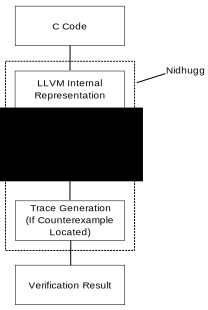
\includegraphics{formal/nidhugg}}
\caption{Nidhugg Processing Flow}
\label{fig:formal:Nidhugg Processing Flow}
\end{figure}

Although the jury is still out on this question, stateless model
checkers such as Nidhugg~\cite{CarlLeonardsson2014Nidhugg} have in
some cases handled larger programs~\cite{SMC-TreeRCU}, and with
similar ease of use, as illustrated by
Figure~\ref{fig:formal:Nidhugg Processing Flow}.
In addition, Nidhugg was more than an order of magnitude faster than
was \co{cbmc} for some Linux-kernel RCU verification scenarios.
Of course, Nidhugg's speed and scalability advantages are tied to
the fact that it does not handle data non-determinism, but this
was not a factor in these particular verification scenarios.

Nevertheless, as with \co{cbmc}, Nidhugg has not yet been able to
locate a bug that Linux-kernel RCU's maintainer was not already
aware of.
However, it was able to demonstrate that one historical bug in
Linux-kernel RCU was fixed by a different commit than the maintainer
thought, which gives some additional hope that stateless model checkers
like Nidhugg might someday be useful for finding concurrency bugs in
parallel code.


\section{Summary}
\label{sec:formal:Summary}

이 챕터에서 설명한 형식적 검증 테크닉은 작은 병렬 알고리즘들을 검증하는데에는
매우 강력한 도구입니다만, 당신의 도구상자에 그것들만 있어선 안됩니다.
지난 수십년간의 형식적 검증에 대한 집중에도 불구하고, 테스트는 커다란 병렬
소프트웨어 시스템을 위한 대표적 검증 도구로
남아있습니다~\cite{JonathanCorbet2006lockdep,DaveJones2011Trinity,PaulEMcKenney2016Formal}.
\iffalse

The formal-verification techniques described in this chapter
are very powerful tools for validating small
parallel algorithms, but they should not be the only tools in your toolbox.
Despite decades of focus on formal verification, testing remains the
validation workhorse for large parallel software
systems~\cite{JonathanCorbet2006lockdep,DaveJones2011Trinity,PaulEMcKenney2016Formal}.
\fi

물론 이는 항상 그렇지는 않을 수도 있는 것이 사실입니다.
이를 확실히 하기 위해, 2017년 기준으로 200억개가 넘는 리눅스 커널의
인스턴스가 존재한다고 추정된다는 점을 생각해 보세요.
리눅스 커널에 평균적으로 백만년의 수행 중 한번 발생할 수 있는 버그가 있다고
생각해 봅시다.
앞의 챕터의 마지막에서 설명했다시피, 이 버그는 이 전체 설치된 환경에서
\emph{하루에} 50 번씩 나타날 겁니다.
하지만 대부분의 형식적 검증 테크닉은 매우 작은 코드에 대해서만 사용될 수 있다는
사실도 여전합니다.
그런 상황에서 동시적 코드를 짜는 사람들은 뭘 해야 할까요?
\iffalse

It is nevertheless quite possible that this will not always be the case.
To see this, consider that there is estimated to be more than twenty
billion instances of the Linux kernel as of 2017.
Suppose that the Linux kernel has a bug that manifests on average every million
years of runtime.
As noted at the end of the preceding chapter, this bug will be appearing
more than 50 times \emph{per day} across the installed base.
But the fact remains that most formal validation techniques can be used
only on very small code bases.
So what is a concurrency coder to do?
\fi

한가지 방법은 첫번째 버그, 첫번째로 관련있는 버그, 마지막으로 관련있는 버그,
그리고 마지막 버그를 찾는 것에 대해 생각해 보는 겁니다.

첫번째 버그는 코드 검사난 컴파일러의 조사를 통해 발견되어집니다.
최신의 컴파일러에 의해 제공되는, 지속적으로 세련되어지는 진단 기능이 가벼운
형태의 형식적 검증으로 여겨질 수도 있긴 하지만, 그것들을 그런 용어로 부르는건
흔하지 않습니다.
이는 부분적으로는 ``내가 그걸 사용하고 있다면, 그것은 형식적 검증일 수 없다''
라고 말하는, 이상한 실무자의 선입견 때문이기도 하고, 컴파일러 진단기능과 검증에
대한 연구 사이의 서로 다른 철학 때문이기도 합니다.
\iffalse

One approach is to think in terms of finding the first bug, the first
relevant bug, the last relevant bug, and the last bug.

The first bug is normally found via inspection or compiler diagnostics.
Although the increasingly sophisticated diagnostics provided by modern
compilers might be considered to be a lightweight sort of formal
verification, it is not common to think of them in those terms.
This is in part due to an odd practitioner prejudice which says
``If I am using it, it cannot be formal verification'' on the one
hand, and the large difference in sophistication between compiler
diagnostics and verification research on the other.
\fi

첫번째로 관련있는 버그는 코드 검사나 컴파일러 진단 기능으로 발견되어질 수도
있지만, 이 두 단계가 오타와 거짓 양성 반응만을 찾게 되는 것도 흔하지 않은 일은
아닙니다.
어떤 방식으로든, 실제 제품에서마주하게 될 버그들인 관련된 많은 버그들은 많은
경우 테스트를 통해 발견되어질 겁니다.

테스트가 예측된 사용 예에서 만들어졌든 진짜 사용 예에서 만들어졌든, 마지막
연관된 버그가 테스트를 통해 발견되어지는 것은 흔치 않은 일이 아닙니다.
이 상황은 형식적 검증에 대한 완전한 거부의 동기가 될 수도 있겠습니다만,
관계없는 버그들은 black-hat 공격의 덕에 최소한의 알맞은 사이즈에 있어서는
갑자기 관계있는 것이 되어버리는 안좋은 습관을 가지고 있습니다.
전체 소프트웨어 가운데 그 분포도를 지속적으로 높여가는 보안에 관련된
소프트웨어에 있어서는 마지막 버그를 찾아내고 고쳐내려는 강한 동기가 존재할 수
있습니다.
테스트는 마지막 버그를 찾아내는 것은 명백히 불가능하므로 형식적 검증에게만
가능한 역할이 존재합니다.
형식적 검증이 그 안으로 적용될 수 있다고만 하면 그런 역할이 있다는
이야기입니다.
이 챕터에서 보였듯이, 현재의 형식적 검증 시스템들은 상당히 제한적입니다.
\iffalse

Although the first relevant bug might be located via inspection or
compiler diagnostics, it is not unusual for these two steps to find
only typos and false positives.
Either way, the bulk of the relevant bugs, that is, those bugs that
might actually be encountered in production, will often be found via testing.

When testing is driven by anticipated or real use cases, it is not
uncommon for the last relevant bug to be located by testing.
This situation might motivate a complete rejection of formal verification,
however, irrelevant bugs have an annoying habit of suddenly becoming relevant
at the least convenient moment possible, courtesy of black-hat attacks.
For security-critical software, which appears to be a continually
increasing fraction of the total, there can thus be strong motivation
to find and fix the last bug.
Testing is demonstrably unable to find the last bug, so there is a
possible role for formal verification.
That is, there is such a role if and only if formal verification
proves capable of growing into it.
As this chapter has shown, current formal verification systems are
extremely limited.
\fi

\QuickQuiz{}
	하지만 충분히 낮은 단계의 소프트웨어는 모든 의도와 목적에 있어
	블랙햇으로부터의 공격에 내성이 있지 않나요?
	\iffalse

	But shouldn't sufficiently low-level software be for all intents
	and purposes immune to being exploited by black hats?
	\fi
\QuickQuizAnswer{
	불행히도, 그렇지 않습니다.

	한번은, Paul E. McKenney 는 리눅스 커널 RCU 가 그런 공격에 대해 내성이
	있다고 생각했는데, Row Hanner 의 발전은 그렇지 않음을 보였습니다.
	무엇보다도, 그 블랙햇들이 시스템의 DRAM 을 건들 수 있다면, RCU 를 건들
	수 있습니다.
	\iffalse

	Unfortunately, no.

	At one time, Paul E. McKenney felt that Linux-kernel RCU
	was immune to such exploits, but the advent of Row Hammer
	showed him otherwise.
	After all, if the black hats can hit the system's DRAM,
	they can hit RCU.
	\fi
} \QuickQuizEnd

또다른 방법은 형식적 검증이 많은 경우 테스트보다 적용하기가 어렵다는 점을
고려하는 겁니다.
물론 이는 문화적인 측면에서의 이야기일 수 있고, 형식적 검증이 더 많은
사람들에게 친숙해 질수록 더 쉽게 전파될 것이라는 희망을 가져볼 수도 있습니다.
그렇다고는 하나, 매우 간단한 테스트 사용은 임의의 거대한 소프트웨어 시스템에서
심각한 버그들을 찾아낼 수 있습니다.
반면에, 형식적 검증을 적용하기 위해 필요한 노력은 시스템의 크기가 증가할수록
극적으로 증가합니다.

전 20년이 넘도록 형식적 검증을 형식적 검증이 효력을 발휘하는 곳에서 필요할
때에만 사용했을 뿐인데, 설계 시점에서의, 무엇보다 중요한 소프트웨어 구성물의
작고 복잡한 부분의 검증에 있어 그랬습니다.
무엇보다 중요하지만 더 커다란 소프트웨어 구성물들은 물론 테스트로 검증했습니다.
\iffalse

Another approach is to consider that
formal verification is often much harder to use than is testing.
This is of course in part a cultural statement, and there is every reason
to hope that formal verification will be perceived to be easier as more
people become familiar with it.
That said, very simple test harnesses can find significant bugs in arbitrarily
large software systems.
In contrast, the effort required to apply formal verification seems to
increase dramatically as the system size increases.

I have nevertheless made occasional use of formal verification
for more than 20 years, playing to formal verification's strengths,
namely design-time verification of small complex portions of the overarching
software construct.
The larger overarching software construct is of course validated by testing.
\fi

\QuickQuiz{}
	L4 마이크로커널의 전체 검증을 생각해 보면, 이런 형식적 검증에 대한
	제한적인 시각은 약간 시대에 뒤쳐진 것 아닌가요?
	\iffalse

	In light of the full verification of the L4 microkernel,
	isn't this limited view of formal verification just a little
	bit obsolete?
	\fi
\QuickQuizAnswer{
	안타깝지만, 그렇지 않습니다.

	L4 마이크로커널의 첫번째 전체 검증은 많은 수의 Ph.D.~학생들 학생마다
	매우 느린 속도로 진행한, 손으로 하는 코드 검증으로 이루어진
	역작이었습니다.
	이런 수준의 노력은 대부분의 소프트웨어 프로젝트들에는 적용될 수가
	없는데, 변화의 비율이 너무 거대하기 때문입니다.
	더 나아가서, 비록 L4 마이크로커널이 형식적 검증의 시점에서 보기에는
	커다란 소프트웨어 작품이긴 합니다만, LLVM, \GCC, 리눅스 커널, Hadoop,
	MongoDB, 그 외의 커다란 많은 것들 등과 같은 많은 수의 프로젝트들에
	비교하면 매우 작은 것입니다.
	또한, 이 검증은 일부 연구자들이 인정했듯이, 한계를 가지고 있습니다:
	\url{https://wiki.sel4.systems/FrequentlyAskedQuestions#Does_seL4_have_zero_bugs.3F}.
	\iffalse

	Unfortunately, no.

	The first full verification of the L4 microkernel was a tour de force,
	with a large number of Ph.D.~students hand-verifying code at a
	very slow per-student rate.
	This level of effort could not be applied to most software projects
	because the rate of change is just too great.
	Furthermore, although the L4 microkernel is a large software
	artifact from the viewpoint of formal verification, it is tiny
	compared to a great number of projects, including LLVM,
	\GCC, the Linux kernel, Hadoop, MongoDB, and a great many others.
	In addition, this verification did have limits, as the researchers
	freely admit, to their credit:
	\url{https://wiki.sel4.systems/FrequentlyAskedQuestions#Does_seL4_have_zero_bugs.3F}.
	\fi

	형식적 검증이 마침내 더 최근의, 커다란 수준의 자동화에 관련된 L4 검증을
	포함해서 어떤 전망을 내놓기 시작하고 있기는 하지만, 전망 가능한 미래에
	테스트를 완전히 대체할 기회는 현재로써는 보이지 않습니다.
	그리고 이 점에 있어서 제가 틀렸다고 증명되면 전 좋아할 겁니다만, 그런
	증명은 실제 소프트웨어를 검증하는 실제 도구를 통한 형태여야 하지,
	자극적인 미사여구를 통한 형태가 되어선 안될 겁니다.
	\iffalse

	Although formal verification is finally starting to show some
	promise, including more-recent L4 verifications involving greater
	levels of automation, it currently has no chance of completely
	displacing testing in the foreseeable future.
	And although I would dearly love to be proven wrong on this point,
	please note that such a proof will be in the form of a real tool
	that verifies real software, not in the form of a large body of
	rousing rhetoric.
	\fi

	% TODO: Apply
	Perhaps someday formal verification will be used heavily for
	validation, including for what is now known as regression testing.
	Section~\ref{sec:future:Formal Regression Testing?} looks at
	what would be required to make this possibility a reality.
} \QuickQuizEnd

마지막 방법은 다음의 두개의 정의와 그것들이 암시하는 결론에 대해서 고려해 보는
것입니다:
\iffalse

One final approach is to consider the following two definitions and the
consequence that they imply:
\fi

\begin{description}[itemsep=0pt,labelindent=1em]
\item[정의:]	버그가 없는 프로그램들은 사소한 프로그램들이다.
\item[정의:]	신뢰할 수 있는 프로그램은 알려진 버그가 없다.
\item[결론:]	모든 사소하지 않으며 신뢰할 수 있는 프로그램에는 최소 하나의
		아직 알려지지 않은 버그가 있다.
\iffalse

\item[Definition:]	Bug-free programs are trivial programs.
\item[Definition:]	Reliable programs have no known bugs.
\item[Consequence:]	Any non-trivial reliable program contains at least
			one as-yet-unknown bug.
\fi
\end{description}

이 시점에서 보면, 모든 검증 영역에서의 진보는 두가지 영향을 가질 수밖에 없을
겁니다: (1)~사소한 프로그램들의 갯수의 증가 또는 (2)~신뢰할 수 있는
프로그램들의 수의 감소.
물론, 인류의 멀티코어 시스템과 소프트웨어에 대한 증가하는 의존도는 사소한
프로그램들의 갯수의 가파른 증가에 대한 커다란 동기가 될겁니다!
\iffalse

From this viewpoint, any advances in validation and verification can
have but two effects: (1)~An increase in the number of trivial programs or
(2)~A decrease in the number of reliable programs.
Of course, the human race's increasing reliance on multicore systems and
software provides extreme motivation for a very sharp increase in the
number of trivial programs!
\fi

하지만, 만약 여러분의 코드가 너무 복잡해서 여러분이 형식적 검증 도구에 너무
과하게 의존하고 있다는 점을 알게 된다면, 여러분은 여러분의 설계를 다시 세심하게
생각해 봐야 하는데, 당신의 형식적 검증 도구들이 당신의 코드가 특정 목적 언어로
손으로 변환해야 하게 되는 상황이라면 특히 그렇습니다.
예를 들어,
Section~\ref{sec:formal:Promela Parable: dynticks and Preemptible RCU}
에서 보인 preemption 가능한 RCU 의 복잡한 dynticks 인터페이스 구현에 있어서는
Section~\ref{sec:formal:Simplicity Avoids Formal Verification} 에서
이야기한대로 훨씬 간단한 대안적 구현이 존재함이 드러났습니다.
다른게 모두 동일하다면, 복잡한 구현을 위한 올바름의 증명보다 간단한 구현이 훨씬
낫습니다!

그리고 형식적 검증 테크닉들과 시스템들에 대한 열려있는 도전은 이 요약 내용이
틀리다고 증명하는 것입니다!
이 일을 돕기 위해, Verification Challenge~6 가 사용
가능합니다~\cite{PaulEMcKenney2017VerificationChallenge6}.
한번 보세요!!!
\iffalse

However, if your code is so complex that you find yourself
relying too heavily on formal-verification
tools, you should carefully rethink your design, especially if your
formal-verification tools require your code to be hand-translated
to a special-purpose language.
For example, a complex implementation of the dynticks interface for
preemptible RCU that was presented in
Section~\ref{sec:formal:Promela Parable: dynticks and Preemptible RCU}
turned out to
have a much simpler alternative implementation, as discussed in
Section~\ref{sec:formal:Simplicity Avoids Formal Verification}.
All else being equal, a simpler implementation is much better than
a proof of correctness for a complex implementation!

And the open challenge to those working on formal verification techniques
and systems is to prove this summary wrong!
To assist in this task, Verification Challenge~6 is now
available~\cite{PaulEMcKenney2017VerificationChallenge6}.
Have at it!!!
\fi
